\documentclass[UTF8,a4paper,12pt]{ctexart}
\usepackage[margin=2.35cm]{geometry}
\usepackage{graphicx,booktabs,longtable,tabularx,array,calc}
\usepackage{amsmath,amssymb,enumitem,caption,fancyhdr,float,dirtree}
\usepackage{algorithm,algpseudocode}
\usepackage{listings}
\usepackage[hidelinks]{hyperref}
\usepackage{xcolor,tikz,pgfplots}
\usepackage{seqsplit}
\usetikzlibrary{arrows.meta,positioning,calc,shapes.geometric,fit,backgrounds}
\pgfplotsset{compat=1.18}

\setcounter{tocdepth}{3}
\setlength{\parindent}{2em}
\setlength{\parskip}{0.32em}
\setlist{itemsep=0.2em,topsep=0.35em,parsep=0pt,partopsep=0pt}
\sloppy
\renewcommand{\arraystretch}{1.25}
\graphicspath{{src/assets/}{assets/}}
\captionsetup{font=small,labelfont=bf,position=bottom}
\captionsetup[table]{position=top,skip=6pt}
\floatname{algorithm}{算法}
\captionsetup[algorithm]{font=small,labelfont=bf,position=top,skip=4pt}
\pagestyle{fancy}
\fancyhf{}
\fancyfoot[C]{\thepage}
\renewcommand{\headrulewidth}{0pt}
\newcolumntype{Y}{>{\raggedright\arraybackslash}X}
\newcolumntype{C}[1]{>{\centering\arraybackslash}p{#1}}
\newcommand{\code}[1]{\texttt{\seqsplit{#1}}}
\newcommand{\TopStack}[1]{\begin{tabular}[t]{@{}l@{}}#1\end{tabular}}
\newcommand{\evidence}[1]{\textsuperscript{\textcolor{blue!60!black}{[#1]}}}
\newcommand{\MetricPending}[1]{\textcolor{orange!75!black}{\textbf{[\,待补：#1\,]}}}
\definecolor{codekeyword}{RGB}{28,79,145}
\definecolor{codecomment}{RGB}{42,111,73}
\definecolor{coderegister}{RGB}{135,47,47}
\lstdefinelanguage{RV32Asm}{
  alsoletter={.},
  morekeywords={.insn,add,addi,and,andi,beq,bne,j,lbu,lhu,lw,mul,or,slli,srli,sw,xor},
  morekeywords=[2]{zero,ra,sp,t0,t1,t2,t3,t4,t5,t6,a0,a1,a2,a3,a4,a5,a6,a7},
  morecomment=[l]{\#}
}
\lstdefinestyle{cstatement}{
  language=C,
  basicstyle=\ttfamily\scriptsize,
  keywordstyle=\color{codekeyword}\bfseries,
  commentstyle=\color{codecomment}\itshape,
  stringstyle=\color{violet!70!black},
  frame=none,
  columns=fullflexible,
  keepspaces=true,
  showstringspaces=false,
  breaklines=true,
  aboveskip=3pt,
  belowskip=2pt
}
\lstdefinestyle{rv32statement}{
  language=RV32Asm,
  basicstyle=\ttfamily\scriptsize,
  keywordstyle=\color{codekeyword}\bfseries,
  keywordstyle=[2]\color{coderegister},
  commentstyle=\color{codecomment}\itshape,
  frame=none,
  columns=fullflexible,
  keepspaces=true,
  showstringspaces=false,
  breaklines=true,
  escapeinside={(*@}{@*)},
  aboveskip=3pt,
  belowskip=2pt
}
\newcommand{\CustomInsn}[2]{%
  {\strut\ttfamily\fontsize{6.4}{7.2}\selectfont #1\ \textcolor{codecomment}{\itshape\# #2}}}
\newcommand{\CodeCompareBegin}[2]{%
  \par\noindent\begin{minipage}{\linewidth}
  \hrule height 0.8pt\relax\vspace{2pt}
  \noindent\begin{minipage}[t]{0.48\linewidth}{\small\bfseries #1}\end{minipage}\hfill
  \begin{minipage}[t]{0.48\linewidth}{\small\bfseries #2}\end{minipage}
  \par\vspace{2pt}\hrule height 0.4pt\relax\vspace{1pt}}
\newcommand{\CodeCompareEnd}{%
  \par\vspace{1pt}\hrule height 0.8pt\relax
  \end{minipage}\par\smallskip}
\newcommand{\coverfield}[2]{%
  {\zihao{4}\noindent\makebox[6em][l]{\heiti#1：}%
   \underline{\makebox[\dimexpr\textwidth-6em\relax][l]{\strut\heiti #2}}\par}}
\newenvironment{signalstable}[1]{%
  \scriptsize\begin{longtable}{@{}p{\dimexpr0.17\linewidth-1.36\tabcolsep\relax}
    C{\dimexpr0.07\linewidth-0.56\tabcolsep\relax}
    p{\dimexpr0.14\linewidth-1.12\tabcolsep\relax}
    p{\dimexpr0.17\linewidth-1.36\tabcolsep\relax}
    p{\dimexpr0.45\linewidth-3.60\tabcolsep\relax}@{}}
  \caption{#1}\\\toprule
  \textbf{信号或信号组}&\textbf{方向}&\textbf{位宽/类型}&\textbf{握手关系}&\textbf{作用}\\\midrule\endhead
  \bottomrule\endfoot
}{\end{longtable}\normalsize}

\begin{document}
\begin{titlepage}
  \centering
  
\includegraphics[width=0.35\textwidth]{common/competition-logo.png}\par\vspace{1.2cm}
  {\zihao{2}\bfseries 第十届\\全国大学生集成电路创新创业大赛\par}
  \vspace*{\fill}
  \begin{minipage}{\textwidth}
    \raggedright
    \setlength{\parindent}{0pt}
    \coverfield{报告类型}{决赛技术文档}
    \vspace{0.45cm}
    \coverfield{参赛杯赛}{``竞业达''企业命题}
    \vspace{0.45cm}
    \coverfield{作品名称}{基于RISC-V指令集的CPU设计}
    \vspace{0.45cm}
    \coverfield{队伍编号}{CICC1004252}
    \vspace{0.45cm}
    \coverfield{团队名称}{和溢位}
    \vspace{2cm}
  \end{minipage}
\end{titlepage}

\tableofcontents
\clearpage
\section*{作品核心内容快速预览}
\addcontentsline{toc}{section}{作品核心内容快速预览}

本项目实现了一款面向 FPGA 的 RV32 顺序单发射五级流水处理器。设计以
IFU--IDU--EXU--LSU--WBU 为主流水，在统一反压与控制流重定向机制上集成动态分支预测、
4\,KiB 数据缓存、分区式执行/写回通路、多周期整数扩展和领域自定义指令。技术文档重点给出
处理器结构、接口时序、指令语义、性能与 WNS 演进，以及从指令语义到板级运行的验证闭环。

\PlaceholderFigure{作品核心结构快速预览}{后续替换为团队制作的总决赛核心结构总览图；建议同时标注五级流水、预测器、缓存、多周期单元、自定义指令单元与板级系统。}

\begin{table}[H]
\centering
\caption{核心成果与正文索引}
\small
\begin{tabularx}{\linewidth}{@{}p{0.16\linewidth}Yp{0.16\linewidth}@{}}
\toprule
\textbf{核心内容}&\textbf{快速结论}&\textbf{查阅位置}\\\midrule
处理器架构&五级顺序单发射、ready/valid 反压、epoch 冲刷、分区结果通路&第\ref{sec:architecture}节\\
控制流前端&512 项八 bank LUTRAM BTB、表项 2-bit 方向计数器、2 项返回地址栈&第\ref{sec:frontend}节\\
存储系统&4\,KiB 双 bank 直接映射 D-cache，主数据与 late-load 异步副本协同&第\ref{sec:memory}节\\
指令能力&RV32I、RV32M、Zicsr、机器态控制流、部分 RISC-V B 扩展及自定义指令&第\ref{sec:extensions}节\\
领域加速&CRC 字节更新、位抽取乘法、链式结构变换、矩阵归约、流式状态识别&第\ref{sec:custom}节\\
物理实现&250\,MHz 时序闭合；300\,MHz 完成布局布线并持续进行结构级时序优化&第\ref{sec:timing}节\\
性能演进&同口径正式负载板测由 10.695831\,s 优化至 6.696372\,s，完整过程同时记录 WNS&第\ref{sec:performance}节\\
验证体系&Vivado Simulation、Verilator/NEMU、指令测试、RT-Thread、实现与上板测评闭环&第\ref{sec:verification}节\\
\bottomrule
\end{tabularx}
\end{table}

\noindent\textbf{指标口径说明：}性能折线仅连接采用相同正式负载、相同迭代规模且 CRC 正确的板测记录；
WNS 与其对应实现一一配对。当前设计另在 250\,MHz 下取得 post-route physical optimization
WNS $+0.009$\,ns，在 300\,MHz 下取得 $-0.580$\,ns。不同实现点在正文中分别列示，不拼接为同一结果。

\PlaceholderFigure{总决赛核心结果实物与报告拼图}{建议放置正式板测 UART 输出、开发板运行照片，以及 250\,MHz 和 300\,MHz Timing Summary 的关键区域。}
\clearpage

\section{项目概述与研发演进}\label{sec:overview}

\subsection{项目目标}

本项目面向竞业达指定 FPGA 平台，目标是在受限片上存储与逻辑资源条件下完成一款可综合、可验证、
可上板运行的 RISC-V 处理器。设计同时关注三类约束：其一是指令和机器态控制流的正确性；其二是
顺序流水线在数据相关、访存延迟和控制流重定向下的稳定运行；其三是 FPGA 实现后的频率、资源与
工作负载运行时间。工程使用 Chisel 描述核心 RTL，并通过内联 BlackBox 模型兼顾 Verilator 仿真与
Vivado IP 综合绑定。

\subsection{版本边界与研发演进}

为保证全文可追溯，本文只采用两个明确的版本节点：分赛区后续报告版本为 tag
\code{ReginalFinal-Post-Report-Version}，对应提交 \commit{2b2734bca383dbfcbe840787ab0033e4980775eb}；
总决赛冻结版本为 \commit{fabb5995bdd394578fbf989b6b20d5eae45b320c}。本报告不按提交历史逐项复述
研发过程，而是以冻结版本中仍然存在的结构为准，将演进归纳为表\ref{tab:evolution}所示的成功方向。

\begin{table}[H]
\centering
\caption{从分赛区版本到总决赛冻结版本的主要演进}\label{tab:evolution}
\begin{tabularx}{\linewidth}{@{}p{0.20\linewidth}YY@{}}
\toprule
\textbf{方向}&\textbf{分赛区后续版本}&\textbf{总决赛冻结版本}\\\midrule
控制流预测&较小容量 BTB 与基础方向预测&512 项八 bank BTB、表项 2-bit 动态预测、返回地址栈\\
数据缓存&2\,KiB 直接映射缓存及早期窄加载副本&4\,KiB 双 bank 缓存，主 BRAM 与逐字节异步副本协同\\
执行结构&普通 ALU 与多周期执行结果耦合较多&快速整数、直接、长算术、加速、加载五类结果通路\\
相关处理&EXU/LSU/WBU 通用旁路与有限 late-load&分组编码的相邻结果选择、注册化 late-load 与专用地址通路\\
整数扩展&RV32M 与部分 B 扩展多周期实现&窄乘法 DSP 快通路、短 B 与迭代 B 分流\\
领域能力&无冻结的领域指令体系&CRC、位抽取乘法、链式变换、矩阵归约、流式状态处理指令\\
板级接口&数码管/LED 为主&加入跨时钟 UART 子系统与原始运行记录通道\\
工程闭环&基础打包和实现脚本&输入身份、并发下限、时序摘要、归档和板测流程可追溯\\
\bottomrule
\end{tabularx}
\end{table}

\subsection{设计平台}

处理器目标器件为 Xilinx Kintex-7 XC7K325T-2FFG900，使用 Vivado 2024.2 完成综合、布局布线与
bitstream 生成。仿真侧使用 Verilator/C++ 周期级仿真与 Vivado XSim；NEMU 作为指令级参考模型，
共享差分测试框架负责比较通用寄存器、PC 及相关体系结构状态。板级系统包含 IROM、DRAM、计时器、
LED、数码管与 UART 等资源，处理器通过统一地址映射访问。

\subsection{设计原则}

\begin{itemize}
  \item \textbf{顺序提交：}任何多周期运算、缓存命中或重定向都不得破坏程序顺序可见性。
  \item \textbf{显式握手：}流水级和多周期单元以 ready/valid 表达接受、保持和完成条件。
  \item \textbf{局部化关键路径：}按消费者类型分割结果、地址、分支和加速通路，减少宽多路选择器跨模块传播。
  \item \textbf{保守的一致性：}缓存无法安全合并时失效对应行；较新 store 优先于较早 load 回填。
  \item \textbf{证据可归属：}提交、输入镜像、频率、实现报告和运行输出必须能够组成同一候选的证据链。
\end{itemize}


\section{CPU 架构与模块设计}\label{sec:architecture}

\subsection{总体架构}

CPU 采用 IFU、IDU、EXU、LSU、WBU 五级顺序单发射流水线。级间寄存器采用 Decoupled
ready/valid 语义：后级不能接收时，前级保持当前 payload；操作真正完成时才发生 \code{fire}。
控制流错误通过 epoch 翻转使年轻指令局部失效，并由注册化重定向邮箱把正确 PC 送回 IFU。

\begin{figure}[H]\centering\resizebox{\linewidth}{!}{%
\begin{tikzpicture}[s/.style={draw,rounded corners,minimum width=2.15cm,minimum height=1cm,align=center,fill=blue!6},q/.style={draw,minimum width=1.05cm,minimum height=0.65cm,fill=gray!8},a/.style={-Stealth,thick},font=\small]
\node[s] (i0) {IFU}; \node[q,right=0.25cm of i0] (q0) {IF/ID}; \node[s,right=0.25cm of q0] (i1) {IDU};
\node[q,right=0.25cm of i1] (q1) {ID/EX}; \node[s,right=0.25cm of q1] (i2) {EXU}; \node[q,right=0.25cm of i2] (q2) {EX/LS};
\node[s,right=0.25cm of q2] (i3) {LSU}; \node[q,right=0.25cm of i3] (q3) {LS/WB}; \node[s,right=0.25cm of q3] (i4) {WBU};
\foreach \x/\y in {i0/q0,q0/i1,i1/q1,q1/i2,i2/q2,q2/i3,i3/q3,q3/i4}{\draw[a] (\x)--(\y);}
\draw[a,red!70!black] (i2.south) -- ++(0,-0.65) -| node[pos=0.2,below]{redirect + epoch} (i0.south);
\draw[a,green!50!black] (i4.north) -- ++(0,0.65) -| node[pos=0.25,above]{写回/旁路状态} (i1.north);
\end{tikzpicture}}\caption{五级流水、反压与重定向关系}\end{figure}


\subsection{IFU 取指模块}

IFU 将 PC、预测信息和流水 epoch 与读取到的指令组合为 \code{FetchedInst}。它能够在消费当前取指响应的
同一周期接受下一 PC 并发出下一请求，从而隐藏片上 IROM 的同步读延迟。若存储或 IDU 反压，则内部
pending 状态保持请求及其预测元信息，避免地址与预测结果错配。

\begin{signalstable}{IFU 接口信号说明}
pc&输入&32 位 Decoupled&\code{valid/ready}&接收待取指 PC\\
predNext&输入&PredBundle&与 PC 同周期&该 PC 对应的预测命中、方向和下一地址\\
epoch&输入&Bool&随 PC 采样&标记当前有效控制流世代\\
mem&输出&SimpleBus master&请求/响应握手&访问 IROM\\
out&输出&FetchedInst Decoupled&\code{valid/ready}&向 IDU 输出指令、PC、预测和 epoch\\
\end{signalstable}

\subsection{IDU 译码与相关处理模块}

IDU 完成指令格式/类型译码、立即数形成、寄存器读取和相关判定。它分别观察 EXU、LSU、WBU 的生产者
状态：目的寄存器匹配且数据已就绪时旁路；匹配但数据无效时停顿。冻结版本进一步把相邻快速结果按
8 个四位组编码，只允许普通整数、分支和 store-data 等短路径消费者使用；地址、M/B、自定义指令和
CSR 等消费者走注册化或保守停顿路径，以限制选择信号扇出。

\begin{signalstable}{IDU 接口信号说明}
in&输入&FetchedInst Decoupled&\code{valid/ready}&接收 IFU 结果\\
rvec&输出/输入&2 读端口 GPR&组合读&给出 rs1/rs2 地址并取得寄存器值\\
csrRead&输出/输入&CSR 单读口&组合读&读取当前 CSR 数据\\
wrBackInfo&输入&三级前递信息组&生产者有效性&判定旁路或停顿\\
lateLoadProducer&输入&延迟加载生产者信息&专用相关协议&标识可延后到 EXU 解析的 load 生产者\\
pipelineFlush&输入&Bool&高有效&丢弃错误 epoch 指令\\
out&输出&DecodedInst Decoupled&\code{valid/ready}&输出操作数、控制元信息和结果类别\\
\end{signalstable}

\begin{figure}[H]\centering
\begin{tikzpicture}[b/.style={draw,rounded corners,align=center,minimum width=2.5cm,minimum height=0.75cm,fill=blue!5},d/.style={draw,diamond,aspect=2,align=center,fill=orange!6},a/.style={-Stealth,thick},font=\small]
\node[b] (src) {源寄存器号}; \node[b,below=0.7cm of src] (p) {EXU/LSU/WBU 生产者优先级}; \node[d,below=0.8cm of p] (m) {目的寄存器匹配？};
\node[b,below left=0.9cm and 1.4cm of m] (g) {使用 GPR 数据}; \node[d,below right=0.9cm and 1.4cm of m] (v) {数据有效？};
\node[b,below left=0.9cm and 1.2cm of v] (s) {停顿}; \node[b,below right=0.9cm and 1.2cm of v] (f) {按消费者选择旁路};
\draw[a] (src)--(p);\draw[a](p)--(m);\draw[a](m)--node[above]{否}(g);\draw[a](m)--node[above]{是}(v);\draw[a](v)--node[above]{否}(s);\draw[a](v)--node[above]{是}(f);
\end{tikzpicture}\caption{IDU 相关判定与旁路流程}\end{figure}



\subsection{EXU 分区执行模块}

EXU 同时承担普通算术、分支裁决、地址请求、多周期整数扩展、CSR 操作和自定义指令执行。为避免所有
结果汇入同一宽 Mux，冻结版本把写回语义划分为 \code{fastInt}、\code{direct}、
\code{longArithmetic}、\code{accelerator} 和 \code{load} 五类。普通整数进入独立快速 ALU；
乘除法、迭代 B 扩展和短 B 运算进入特殊执行簇；领域单元使用独立结果通路；load 最终由存储响应产生。

\begin{signalstable}{EXU 接口信号说明}
in&输入&DecodedInst Decoupled&\code{valid/ready}&接收译码结果及消费者类型\\
previousStageFwd&输入&FastForwardInfo&局部组合选择&只供允许的相邻快速消费者使用\\
lateLoadLSU/WBU&输入&LateLoadInfo&有效/数据有效&在 EXU 注册边界解析受限 load-use\\
dcache&双向&DCache 查询/更新组&查询与更新协议&命中、同步/异步数据及 store 变更\\
memReq/memResp&双向&Decoupled/Valid&请求/响应&普通访存和自定义单元访存\\
fwd&输出&ForwardInfo&生产者状态&向 IDU 广告目的寄存器及数据有效性\\
out&输出&LSUInput Decoupled&\code{valid/ready}&输出分区写回结果、访存和重定向元信息\\
branch* / btbUpdate*&输出&控制流更新组&随完成采样&提供真实方向、目标和表项类型\\
\end{signalstable}

\begin{figure}[H]\centering
\begin{tikzpicture}[u/.style={draw,rounded corners=1.2pt,align=center,minimum width=2.55cm,minimum height=0.78cm},a/.style={-Stealth,thick},font=\small]
\node[u,fill=blue!6,minimum height=5.25cm] (d) {DecodedInst\\按 ResultKind 分发};
\node[u,fill=green!7,right=1.35cm of d,yshift=2.25cm] (fi) {快速整数通路};
\node[u,fill=green!7,right=1.35cm of d,yshift=1.12cm] (di) {直接结果通路};
\node[u,fill=orange!8,right=1.35cm of d] (la) {长算术通路};
\node[u,fill=purple!7,right=1.35cm of d,yshift=-1.12cm] (ac) {硬件加速通路};
\node[u,fill=cyan!7,right=1.35cm of d,yshift=-2.25cm] (ld) {加载结果通路};
\node[u,fill=gray!10,right=2.35cm of la,minimum height=5.25cm] (wb) {按 ResultKind\\局部汇聚与写回};
\draw[a] ([yshift=2.25cm]d.east)--(fi.west);
\draw[a] ([yshift=1.12cm]d.east)--(di.west);
\draw[a] (d.east)--(la.west);
\draw[a] ([yshift=-1.12cm]d.east)--(ac.west);
\draw[a] ([yshift=-2.25cm]d.east)--(ld.west);
\draw[a] (fi.east)--([yshift=2.25cm]wb.west);
\draw[a] (di.east)--([yshift=1.12cm]wb.west);
\draw[a] (la.east)--(wb.west);
\draw[a] (ac.east)--([yshift=-1.12cm]wb.west);
\draw[a] (ld.east)--([yshift=-2.25cm]wb.west);
\end{tikzpicture}\caption{EXU 与写回结果通路分区}\end{figure}


\subsection{LSU 与 WBU}

LSU 保存访存类型、地址低位、缓存命中和分区写回信息，并在同步缓存数据到达后形成 LSU 级旁路。
WBU 对 load 返回字按 \code{func3} 和地址偏移完成字节/半字抽取与符号扩展，随后写入 GPR；其他结果
按结果类别选择后顺序提交。store 的缓存更新在 EXU 请求侧发生，较早 load 的回填则由 store epoch
阻止覆盖更新后的缓存状态。

\begin{signalstable}{LSU 接口信号说明}
in&输入&LSUInput Decoupled&\code{valid/ready}&接收执行结果和访存元信息\\
dcacheReadData&输入&UInt(32)&同步 BRAM 返回&取得上一周期查询的数据\\
fwd&输出&ForwardInfo&生产者状态&向 IDU 提供 LSU 级普通结果状态\\
out&输出&WBUInput Decoupled&\code{valid/ready}&向 WBU 传递统一提交信息\\
\end{signalstable}

\begin{signalstable}{WBU 接口信号说明}
in&输入&WBUInput Decoupled&\code{valid/ready}&接收 LSU 输出\\
memResp&输入&Valid[UInt(32)]&与 load 对齐&接收 DRAM 返回数据\\
dcacheUpdate*&输出&地址/数据/掩码&提交时回填&将有效 load 结果写入缓存\\
gpr&输出&GPR WriteIO&最终提交&写入目的通用寄存器\\
\end{signalstable}

\subsection{GPR 与 CSR}

通用寄存器堆使用两份 32$\times$32 分布式存储器形成双异步读、单同步写结构；写回同址时使用显式
write-through，\code{x0} 始终返回零。CSR 单元实现 \code{mstatus}、\code{mtvec}、\code{mepc}、
\code{mcause}、\code{mcycle} 等机器态状态。冻结版本将 CSR 事务局部化到 EXU，以减少跨越 IDU、
LSU 和 WBU 的读写控制通路。

\subsection{控制流前端}\label{sec:frontend}

BTB 包含 512 个表项，按 8 个 bank、每 bank 64 项组织为异步 LUTRAM。表项保存类型、tag、压缩目标和
2-bit 饱和方向计数器；更新 shadow 保存较窄的 tag/类型/方向状态。复位阶段逐项清零，在初始化完成前
强制查询 miss。新出现且实际不跳转的条件分支不会驱逐同索引下的有用目标。返回预测由 2 项 RAS
提供，call 压入 \code{pc+4}，标准 return 弹出栈顶。

\begin{signalstable}{BTB 与分支预测器接口信号说明}
query.addr&输入&UInt(32)&组合查询&当前推测 PC\\
query.hit/target&输出&Bool/UInt(32)&组合返回&命中与预测目标\\
query.is*&输出&类型/方向组&随查询返回&区分 branch、JAL、return 及预测方向\\
update.*&输入&地址/目标/类型/方向&注册后写入&用真实执行结果训练表项\\
pred&输出&PredBundle&送入 IFU&给出命中、taken 和下一 PC\\
\end{signalstable}

\begin{figure}[H]\centering\resizebox{0.98\linewidth}{!}{%
\begin{tikzpicture}[
 b/.style={draw,rounded corners=1.2pt,align=center,minimum height=0.82cm,fill=blue!6},
 a/.style={-Stealth,thick},font=\small]
\node[b,minimum width=2.0cm] (pc) at (0,1.9) {推测 PC};
\node[b,minimum width=2.45cm] (split) at (3.0,1.9) {\texttt{pc[16:2]}\\tag / bank / 行号};
\node[b,minimum width=5.6cm,minimum height=1.9cm,fill=green!7] (array) at (8.3,1.9) {
  \textbf{8-bank 并行查询阵列}\\[-0.1em]
  bank 0 \quad bank 1 \quad $\cdots$ \quad bank 6 \quad bank 7\\
  每 bank 64 项，LUTRAM 异步读};
\node[b,minimum width=2.9cm] (pick) at (14.4,1.9) {\texttt{pc[10:8]} 选择 bank\\tag 比较并取出表项};

\node[b,minimum width=3.2cm,fill=orange!8] (decode) at (8.0,-0.55) {类型译码\\JAL / branch / return};
\node[b,minimum width=3.4cm,fill=purple!7] (counter) at (14.0,-0.55) {表项 2-bit 饱和计数器\\最高位给出 branch 方向};
\node[b,minimum width=3.2cm,fill=cyan!7] (ras) at (8.0,-2.8) {2 项返回地址栈\\call 压入，return 弹出};
\node[b,minimum width=4.4cm,fill=gray!10] (next) at (14.0,-2.8) {按类型、方向与 RAS 状态选择\\BTB 目标 / RAS 栈顶 / $pc+4$\\形成 PredBundle};

\draw[a] (pc)--(split);
\draw[a] (split)--(array);
\draw[a] (array)--(pick);
\draw[a] (pick.south west) -- ++(0,-0.42) -| (decode.north);
\draw[a] (pick.south east) -- ++(0,-0.42) -| (counter.north);
\draw[a] (decode)--(ras);
\draw[a] (decode.south east) -- ++(0,-0.36) -| ([xshift=-0.75cm]next.north) -- (next.north);
\draw[a] (counter.south) -- ++(0,-0.42) -| ([xshift=0.75cm]next.north);
\draw[a] (ras)--(next);
\end{tikzpicture}}
\caption{512 项 8-bank BTB 与返回预测结构}\end{figure}


\subsection{存储系统与 D-cache}\label{sec:memory}

D-cache 为 4\,KiB 直接映射结构，由两个 512$\times$32 BRAM bank 组成。tag 使用两个 512$\times$8
分布式存储器；bank 位留在存储地址之外。主数据端是单周期同步读，因此 bank 选择也延迟一拍。
另有每 bank 四个逐字节分布式存储器镜像，提供异步 late-load 数据；该数据必须先跨越 EXU--LSU
寄存边界，再参与受限消费者的运算或比较。

\begin{signalstable}{D-cache 接口信号说明}
queryIndex/tag&输入&10/7 bit&组合 tag 查询&普通 load/store 地址\\
lateQueryIndex&输入&10 bit&异步数据查询&late-load 专用地址\\
hit/readData&输出&Bool/UInt(32)&tag 组合、数据同步&普通缓存命中与主数据\\
lateReadData&输出&UInt(32)&异步读取&逐字节副本数据\\
storeUpdate/*&输入&地址/数据/4-bit mask&store 优先&更新或保守失效缓存行\\
update/*&输入&地址/数据/valid/mask&回填协议&写入较早 load 返回或加速单元更新\\
\end{signalstable}

\begin{figure}[H]\centering\resizebox{\linewidth}{!}{%
\begin{tikzpicture}[
 m/.style={draw,rounded corners=1.2pt,align=center,minimum height=1.0cm,inner sep=5pt},
 a/.style={-Stealth,thick},wa/.style={-Stealth,thick,dashed},font=\small]
\node[m,fill=blue!6,text width=3.35cm] (addr) at (0,2.4)
  {普通访问地址\\tag=[17:11]，bank=[11]\\行=[10:2]};
\node[m,fill=green!7,text width=3.75cm] (tags) at (4.8,2.4)
  {普通 tag LUTRAM\\valid + 7-bit tag，C0 比较};
\node[m,fill=green!7,text width=3.9cm] (main) at (10.1,2.4)
  {双 bank 主数据 BRAM\\每 bank 512$\times$32，C1 同步读};
\node[m,fill=gray!10,text width=3.65cm] (normal) at (15.3,2.4)
  {普通 load 命中\\LSU 对齐、扩展并前递};

\node[m,fill=orange!8,text width=4.05cm] (listaddr) at (0,-0.5)
  {\code{xlistfind} 私有查询\\并行地址 node 与 node+4};
\node[m,fill=orange!8,text width=4.15cm] (replica) at (5.4,-0.5)
  {两组 tag/data 异步副本\\每 bank 四块 512$\times$8 数据 RAM};
\node[m,fill=cyan!8,text width=4.0cm] (walker) at (10.9,-0.5)
  {查找器局部寄存器与状态机\\next/info/data 分阶段解析};
\node[m,fill=cyan!8,text width=3.65cm] (listbus) at (16.0,-0.5)
  {副本 miss\\复用统一数据总线};

\node[m,fill=purple!7,text width=5.35cm] (write) at (3.1,-3.5)
  {注册化统一写口：整字分配 / 窄写失效\\miss 回填 / 硬件加速更新};
\node[m,fill=purple!3,text width=5.1cm] (broadcast) at (10.2,-3.5)
  {同一地址、数据与字节掩码\\更新普通阵列与链表查询副本};

\draw[a] (addr.east) -- (tags.west);
\draw[a] (tags)--node[above]{hit}(main);
\draw[a] (main)--(normal);
\draw[a] (listaddr)--(replica);
\draw[a] (replica)--(walker);
\draw[a] (walker)--node[above]{miss}(listbus);
\draw[a] (write)--(broadcast);
\draw[wa] ([xshift=-1.0cm]broadcast.north) -- ++(0,0.55) -| (replica.south);
\draw[wa] (write.west) -- ++(-3.1,0) -- ++(0,7.7) -| (tags.north);
\draw[wa] (broadcast.east) -- ++(5.6,0) -- ++(0,8.1) -| (main.north);
\end{tikzpicture}}
\caption{总容量 4 KiB 的双 bank D-cache：同步普通加载与链表查找镜像副本}\end{figure}


\subsection{SoC、内存接口与 UART}

CPU 核心通过独立取指与数据 SimpleBus 端口接入 JYD SoC。IROM 基址为 \code{0x80000000}，DRAM
基址为 \code{0x80100000}，MMIO 位于 \code{0x80200000} 区域。FPGA 顶层使用 Vivado BRAM IP
承载指令和数据存储；UART 通过 AXI UARTLite、时钟转换和异步字节 FIFO 连接 CPU 与板级 50\,MHz
外设时钟域，使长时间运行能够留下原始、可机器读取的输出。

\begin{signalstable}{SimpleBus 与 SoC 外设接口信号说明}
req.valid/ready&双向&Bool&请求握手&表示一次请求被接受\\
req.addr&输出&UInt(32)&随请求稳定&统一物理地址\\
wen/data/mask&输出&Bool/32/4 bit&写请求有效&表达 store 数据与字节使能\\
resp.valid/rdata&输入&Bool/UInt(32)&响应握手&返回 load 或取指数据\\
LED/SEG/CNT&输出&设备相关&地址译码&板级显示与计时\\
UART TX/RX&双向&串行字节流&跨时钟 FIFO&输出性能记录并支持交互\\
\end{signalstable}

\clearpage
\section{RT-Thread Nano 系统移植}\label{sec:system-port}

赛题要求在处理器上完成操作系统移植。工程选择 RT-Thread Nano 3.1.5，在
\code{jyd-tests/rtthread-nano} 中保留上游内核，并补充 JYD AbstractMachine 平台适配层、精简配置、
FinSH/msh 命令和链接脚本。内核固定到官方 \code{v3.1.5} 标签对应版本，平台改动以独立源文件和补丁
维护，避免把移植代码直接混入上游内核\evidence{E-RTTNANO}。

移植思路参考南京大学 PA 的 RT-Thread 选做讲义\footnote{\href{https://ysyx.oscc.cc/docs/ics-pa/4.1.html\#rt-thread-\%E9\%80\%89\%E5\%81\%9A}{南京大学 PA：RT-Thread 选做讲义}。}及教学分支
\href{https://github.com/NJU-ProjectN/rt-thread-am}{NJU-ProjectN/rt-thread-am}。该教学分支只把依赖库
替换到 AbstractMachine（AM）裸机环境，不能直接用于本处理器；本项目以官方 Nano 3.1.5 为内核，
根据 JYD 的异常入口、地址空间和串口接口独立编写平台层、上下文切换连接代码及链接配置。本文所说
“参考”是指借鉴 AM 事件和自陷组织方法，不表示直接复用一份可运行的 BSP。相关讲义、教学分支和
AM 工程均列入附录参考资料。

\subsection{启动与基础运行环境}

系统入口先调用 \code{ioe\_init} 初始化 JYD 外设，再建立异常处理环境，依次初始化 Nano 的定时器、
调度器、FinSH/msh 和空闲线程，最后进入 \code{rt\_system\_scheduler\_start}。JYD 平台没有 CLINT，
因此该移植采用协作式调度，不依赖周期时钟中断；线程在主动让出 CPU 或内核要求切换时进入调度路径。

新线程的初始栈通过 AM 的 \code{kcontext} 构造。移植层在栈顶保存入口函数、参数和退出函数，再把
首个 PC 设置为统一的线程包装入口；线程第一次被调度时，包装入口取出参数并调用 Nano 线程函数，
线程返回后再进入其退出处理。这样无需为 Nano 另写一套 RISC-V 上下文布局。

\subsection{基于自陷的上下文切换}

Nano 调度器把当前线程和下一线程的栈指针地址传给 \code{rt\_hw\_context\_switch}。移植层记录这两个
地址后调用 AM 的 \code{yield()}；在 RV32 平台上，\code{yield} 先把 \code{a7} 置为 $-1$，再执行
\code{ecall} 主动产生机器态自陷。异常入口保存通用寄存器、\code{mcause}、\code{mstatus} 和
\code{mepc}，AM 将该事件识别为 \code{EVENT\_YIELD} 并进入 Nano 注册的事件处理函数。

事件处理函数把当前 \code{Context} 写入旧线程的栈指针槽，并返回新线程保存的 \code{Context}。
汇编异常出口随后从新上下文恢复寄存器和 \code{mepc}，通过 \code{mret} 回到新线程。整个切换可以概括为：

\begin{center}
\small
Nano 调度请求 $\rightarrow$ \code{rt\_hw\_context\_switch}
$\rightarrow$ \code{yield/ecall} 自陷 $\rightarrow$ 保存旧上下文
$\rightarrow$ 选择新上下文 $\rightarrow$ \code{mret} 恢复执行
\end{center}

首次启动线程复用同一恢复出口，后续线程切换则保存并恢复实际运行现场。该实现同时覆盖处理器的
\code{mtvec}、\code{mepc}、\code{mcause}、\code{ecall/mret} 和通用寄存器保存恢复路径。

\subsection{控制台、Shell 与链接适配}

Nano 的控制台输出映射到 AM \code{putch}，输入由非阻塞 \code{try\_getch} 提供，不引入完整设备框架
和 POSIX 层。配置保留信号量、精简 \code{rt\_kprintf} 及 FinSH/msh，并提供 \code{version}、
\code{ps}、\code{list\_thread} 和 \code{list\_semaphore} 等基本命令。链接脚本保留 FinSH 的函数与变量
符号表区间；JYD 的 IROM/DRAM 分离镜像和平坦仿真镜像分别使用对应的放置方式。

移植完成后，系统能够进入 \code{msh >}，报告 Nano 3.1.5，并列出 shell、空闲线程和信号量对象。
该运行结果既验证 Nano 本身的启动与命令分派，也为处理器机器态异常和上下文恢复提供系统级负载。

\section{指令扩展与硬件加速}\label{sec:extensions}

\subsection{基础指令能力}

处理器实现 RV32I 整数指令集、RV32M 乘除法指令、Zicsr CSR 访问指令以及机器态异常返回，
并实现了部分 RISC-V 标量 B 扩展指令。表~\ref{tab:implemented-extensions} 按标准扩展名称列出实际
实现范围；这里的指令列表即为本设计支持的子集，不表示已经覆盖对应扩展的全部指令。

\begin{table}[H]\centering\scriptsize
\caption{提交 \texttt{8591368} 的标准扩展能力与已实现指令}\label{tab:implemented-extensions}
\begin{tabularx}{\linewidth}{@{}C{0.095\linewidth}p{0.57\linewidth}Y@{}}
\toprule
\textbf{扩展}&\textbf{已实现的指令或能力}&\textbf{实现通路}\\\midrule
RV32M&\code{mul/mulh/mulhsu/mulhu/div/divu/rem/remu}&DSP 流水乘法与迭代除法\\
Zicsr&\code{csrrw/csrrs/csrrc} 及三种立即数形式&CSR 读改写通路\\
Zba&\code{sh1add/sh2add/sh3add}&单周期移位加法\\
Zbb&\code{clz/ctz/sext.b/sext.h/min/minu/max/maxu/rol/andn/orn/xnor/rev8}&短组合或 32 轮计数通路\\
Zbs&\code{bext/bexti/bset/bseti/bclr/bclri/binv/binvi}&单周期位操作\\
Zbkb&\code{pack}&单周期半字拼接\\
\bottomrule
\end{tabularx}
\normalsize\end{table}

\subsection{乘除法与 B 扩展多周期控制}

乘法器按操作类型选择普通低位、全宽高位或窄操作数快速通路；除法器采用恢复除法，每拍执行移位、
比较与减法，最后单独完成符号修正。当前 RTL 的迭代 B 单元只保留 \code{clz/ctz}，逐位执行 32 轮；
移位加法、符号扩展、最小/最大值、逻辑否定组合、\code{rol} 左旋、字节反序和单比特操作保留在短组合
通路。当前支持范围仅以表~\ref{tab:implemented-extensions} 为准；旧迭代单元中的其余操作不再支持。
\code{pack} 由当前单周期快速整数通路实现。

多周期请求被接受后，流水线相关信息仍保留目的寄存器号，但将 \code{dataValid} 保持为 0；因此依赖
该结果的年轻指令会在 IDU 停顿，而无关指令不会把未完成的数据误认为可前递结果。执行单元寄存最终
结果后置位 \code{dataValid}，待后级 \code{ready} 有效时完成握手并释放占用。该协议统一覆盖乘法、
除法、迭代 B 操作以及后述阻塞式加速单元。

\begin{figure}[H]\centering
\begin{tikzpicture}[s/.style={draw,rounded corners=1.2pt,minimum width=3.1cm,minimum height=0.82cm,align=center,fill=blue!6},d/.style={draw,diamond,aspect=2,align=center,fill=orange!7},a/.style={-Stealth,thick},font=\small]
\node[s] (idle) {Idle：接受多周期指令}; \node[s,below=0.7cm of idle] (busy) {Busy：保持 rd 占用\\dataValid=0};
\node[d,below=0.7cm of busy] (valid) {结果有效？}; \node[d,below=0.8cm of valid] (ready) {后级 ready？};
\node[s,below left=0.8cm and 1.4cm of ready] (hold) {Done：寄存结果}; \node[s,below right=0.8cm and 1.4cm of ready] (emit) {完成握手并释放};
\draw[a](idle)--node[right]{in.fire}(busy);\draw[a](busy)--(valid);\draw[a](valid.west)--++(-1,0)|-node[left]{否}(busy.west);
\draw[a](valid)--node[right]{是}(ready);\draw[a](ready)--node[above]{否}(hold);\draw[a](ready)--node[above]{是}(emit);\draw[a](hold)--(emit);
\end{tikzpicture}\caption{多周期执行单元握手与相关保持}\end{figure}


\subsection{B 扩展的动态热点与性能边界}

本小节记录早期 B 扩展探索的动态剖析，用于解释后续为何将更多热点移入专用硬件单元；其中
\code{clmul/clmulh} 等操作不属于提交 \code{8591368} 当前保留的硬件子集。为区分编译器利用 ISA 后的
指令数变化与具体硬件实现的周期代价，本文采用相同 CoreMark 源码、
\code{-O2} 优化级别和 10,000 次迭代的 NEMU 动态剖析进行 ISA 侧比较。未启用 B 扩展时执行
2,848,523,042 条指令；启用 Zba、Zbb、Zbc 和 Zbs 后执行 2,480,540,948 条，减少
367,982,094 条，即 12.918\%。后者包含 112,742,813 条 B 指令，占该镜像动态指令的 4.545\%。
这两个比例分别表示全程序动态指令缩减和 B 指令在新镜像中的占比，不能直接等同为处理器周期或板级
运行时间的缩减。

表~\ref{tab:b-hotspots} 列出历史全 B 镜像中出现次数最多的操作，并同时标出当前硬件是否保留。
\code{sh1add} 主要承担地址生成；
\code{sext.h}、\code{sh2add} 与 \code{pack/zext.h} 构成第二组热点。GNU 反汇编器会把
\code{pack rd,rs1,x0} 显示为 \code{zext.h}，因此二者合并计数。\code{clmul} 与 \code{clmulh}
各执行 5,840,008 次，合计 11,680,016 次，是 CRC 路径的关键替代操作。

\begin{table}[H]\centering\scriptsize
\caption{CoreMark 10,000 次迭代中的历史 B 指令热点及当前状态}\label{tab:b-hotspots}
\begin{tabularx}{\linewidth}{@{}lrrY@{}}
\toprule
\textbf{操作}&\textbf{动态次数}&\textbf{占全程序动态指令比例}&\textbf{提交 \texttt{8591368} 状态}\\\midrule
\code{sh1add}&60,280,009&2.4301\%&保留\\
\code{sext.h}&16,060,001&0.6474\%&保留\\
\code{sh2add}&12,120,153&0.4886\%&保留\\
\code{pack/zext.h}&10,261,412&0.4137\%&保留，由单周期 \code{pack} 实现\\
\code{clmul}&5,840,008&0.2354\%&移除；其已观测用途由 CRC 专用网络覆盖\\
\code{clmulh}&5,840,008&0.2354\%&移除；其已观测用途由 CRC 专用网络覆盖\\
\code{bext}&2,341,195&0.0944\%&保留\\
\bottomrule
\end{tabularx}
\end{table}

被移除的 \code{clmul/clmulh} 在历史镜像中合计占 0.4708\%，且本次观测到的热点用途集中在 CRC
更新；固定异或网络已覆盖该计算，同时避免保留通用迭代无进位乘法器。
其余被裁掉的迭代操作未进入上述热点集合；当前正式程序在迭代 B 单元中只使用
\code{clz/ctz}，因此删除它们可减少状态、选择和结果汇聚逻辑，不影响当前程序镜像。

1,000 次迭代的扩展子集剖析进一步给出：无 B 扩展为 284,879,140 条，仅启用 Zbc 为
251,874,680 条，启用 Zba、Zbb、Zbc、Zbs 全集为 248,080,124 条。由此可见，该工作负载的大部分
编译器侧收益来自 Zbc；这是历史 ISA 探索结果，不表示当前处理器仍支持 Zbc。全 B 镜像中的
\code{clmul/clmulh} 曾替代 CRC 热点内的大量移位和异或。
因此，在相同 B ISA 下启用 CRC 专用网络时，板测由 10.07521570~s 降至
9.56506582~s，严格同口径增量为 5.0634\%。历史上约 12.37\% 的数字混合了“无 B 软件 CRC”和
“有 B 且启用 CRC 加速”两个变化，不能归因于单一改动。受研发周期限制，本阶段未安排严格完整的
B-only 板级对照测试，因此本文不报告 B 扩展单独带来的板级百分比。

\subsection{专用硬件加速设计}\label{sec:custom}

动态剖析表明，热点主要集中在定宽位运算、局部乘累加、依赖访存和流式状态处理。设计分析分别识别出
地址生成、缓存查询、响应等待、局部计算和顺序提交等关键阶段，并针对各阶段配置专用组合或多周期硬件。
这些单元继续服从 EXU 的阻塞、冲刷与顺序写回协议，不改变输入数据、返回值或存储器可见顺序。

\begin{table}[H]\centering\scriptsize
\caption{专用硬件加速单元及其流水边界}\label{tab:accelerator-units}
\begin{tabularx}{\linewidth}{@{}p{0.19\linewidth}p{0.35\linewidth}p{0.19\linewidth}Y@{}}
\toprule
\textbf{硬件单元}&\textbf{主要结构}&\textbf{执行方式}&\textbf{体系结构边界}\\\midrule
CRC 字节更新&固定 XOR 网络与 16 位状态组合&单周期&无内部状态、无访存\\
窄位域乘法&位域抽取、小位宽乘法与补零&单周期&无内部状态、无访存\\
局部乘累加&窄乘法器与局部累加器&分阶段多周期&结果经长算术通路提交\\
访存型归约&地址生成与局部状态寄存器&阻塞式状态机&只读请求经统一 LSU 发出\\
依赖访存处理&D-cache 专用查询副本、统一请求口&阻塞式状态机&更新遵循普通 store 顺序\\
流式状态处理&对齐字读取与局部状态寄存器&有界多周期&只读输入，结果顺序提交\\
\bottomrule
\end{tabularx}
\normalsize\end{table}

\subsubsection{定宽位运算数据通路}

CRC 单元把一个输入字节与 16 位状态送入固定异或网络，直接得到下一状态；窄位域乘法单元并行完成
字段抽取和小位宽无符号乘法。两者均不保留跨操作状态，也不访问存储器，因此可接入单周期加速结果
通路，避免通用移位、掩码和异或序列反复占用整数数据通路。

\begin{figure}[H]\centering
\begin{tikzpicture}[n/.style={draw,rounded corners=1.2pt,minimum height=0.72cm,minimum width=2.15cm,align=center,fill=blue!6},a/.style={-Stealth,thick},font=\scriptsize,node distance=0.65cm and 0.85cm]
\node[n] (rs) {寄存器操作数\\rs1、rs2};
\node[n,above right=0.35cm and 1.1cm of rs] (crc) {8 位数据 + 16 位状态\\固定 XOR 矩阵};
\node[n,below right=0.35cm and 1.1cm of rs] (bmul) {位域抽取\\4 位 $\times$ 7 位};
\node[n,right=1.2cm of crc] (cz) {16 位 CRC\\高位补零};
\node[n,right=1.2cm of bmul] (bz) {11 位乘积\\高位补零};
\node[n,right=1.2cm of $(cz)!0.5!(bz)$] (wb) {硬件加速通路\\单周期写回};
\draw[a](rs)--(crc); \draw[a](rs)--(bmul); \draw[a](crc)--(cz); \draw[a](bmul)--(bz);
\draw[a](cz)--(wb); \draw[a](bz)--(wb);
\end{tikzpicture}
\caption{\texttt{xcrcu8} 与 \texttt{xbmul} 的定宽单周期数据通路}
\end{figure}


同 ISA 配置和迭代口径的板级对照中，CRC 硬件将运行时间由 10.07521570\,s 降至
9.56506582\,s，缩短 5.0634\%；继续加入窄位域乘法后降至 9.07727378\,s，相对前一点缩短
5.10\%。这两组结果用于说明定宽组合网络的收益，未将其外推到其他程序。

\subsubsection{乘累加与访存型归约}

乘累加单元复用窄 DSP，并在执行单元内部保存局部累加值。硬件按初始化、局部更新和结果整理等阶段
推进，减少中间数据在 GPR 与整数旁路上的往返；多周期握手保证相关消费者只在结果有效后继续执行。

访存型归约单元锁存请求参数后，由地址生成、请求、等待响应、局部变换和完成提交等状态逐拍推进。
每份输入数据仍经统一 LSU/D-cache 接口实际读取，单元不直接访问或旁路存储阵列。

以下四幅状态机图为便于说明控制关系，将多个硬件阶段合并画在同一视图中；
各节点对应独立的多拍步骤或握手边界，并非在一、两拍内直接产生整个操作的结果。

\begin{figure}[H]\centering
\resizebox{\linewidth}{!}{%
\begin{tikzpicture}[n/.style={draw,rounded corners=1.2pt,minimum height=0.78cm,minimum width=2.25cm,align=center,fill=green!7},a/.style={-Stealth,thick},font=\small,node distance=0.7cm]
\node[n] (cfg) {锁存 $base,n,clip$\\清零行列计数};
\node[n,right=of cfg] (req) {地址递增器\\发起 32 位读};
\node[n,right=of req] (resp) {响应寄存\\得到 $C_i$};
\node[n,right=of resp] (calc) {$T_i$、裁剪判断\\趋势计分};
\node[n,right=of calc] (next) {更新 $S_i,P_i,R_i$\\行列计数};
\node[n,right=of next] (done) {符号扩展\\写回 $R$};
\foreach \x/\y in {cfg/req,req/resp,resp/calc,calc/next,next/done}{\draw[a](\x)--(\y);}
\draw[a](next.south)--++(0,-0.45)-|node[pos=0.25,below]{尚有元素}(req.south);
\end{tikzpicture}}
\caption{\texttt{xmsum} 的顺序访存与递推归约流程}
\end{figure}


位域乘法融合版本在同一硬件配置下将板测时间由 6.690732940\,s 降至 6.485317060\,s。
加入局部乘累加状态后，相同 10/100 次 NPC 仿射模型的 10,000 次时间由 5.570051480\,s 降至
5.301518123\,s；该点未形成隔离板测，因此仅作为仿真拟合证据。访存型归约在对应板级对照中将
9.07727378\,s 降至 8.57272290\,s，缩短 5.56\%。

\subsubsection{依赖访存加速}

依赖访存的关键代价是后一次地址需要等待前一次数据。硬件在 D-cache 中设置与普通读取同步的专用查询
副本，并将并行查询、命中解析、统一总线回退、响应等待和完成提交划分为显式状态。设备区访问不会进入
缓存阵列。

\begin{figure}[H]\centering
\resizebox{\linewidth}{!}{%
\begin{tikzpicture}[
  s/.style={draw,rounded corners=1.2pt,align=center,minimum width=2.25cm,minimum height=0.78cm,fill=blue!6},
  d/.style={draw,diamond,aspect=2.15,align=center,fill=orange!8,inner sep=2pt},
  a/.style={-Stealth,thick},font=\scriptsize]
\node[s] (idle) at (6.0,6.5) {idle\\锁存参数};
\node[s] (lookup) at (6.0,5.2) {nodeLookup\\并行查 next/info};
\node[s] (resolve) at (6.0,3.9) {nodeResolve\\解析两路命中};
\node[s] (nextmem) at (2.3,3.0) {nextMemory\\等待 next};
\node[s] (inforeq) at (2.3,1.6) {infoRequest\\发出 info 请求};
\node[s] (infomem) at (6.0,1.6) {infoMemory\\等待 info};
\node[s] (dlookup) at (6.0,0.1) {dataLookup\\查询 $[info]$};
\node[s] (dresolve) at (9.6,0.1) {dataResolve\\解析数据命中};
\node[s] (dmem) at (9.6,-1.7) {dataMemory\\等待数据};
\node[d] (judge) at (6.0,-1.7) {匹配或到尾?};
\node[s] (done) at (2.3,-1.7) {done\\保持返回值};

\draw[a] (idle)--(lookup);
\draw[a] (lookup)--(resolve);
\draw[a] (resolve.west) -- ++(-0.55,0) -| node[pos=0.25,above]{next miss} (nextmem.north);
\draw[a] (resolve)--node[right]{next hit、info miss}(infomem);
\draw[a] (resolve.east) -- ++(0.55,0) -| node[pos=0.65,right]{两者命中} (dresolve.north);
\draw[a] (nextmem)--node[right]{info miss}(inforeq);
\draw[a] (nextmem.west) -- ++(-0.8,0) -- ++(0,-2.9) --
  node[above]{info hit} (dlookup.west);
\draw[a] (inforeq)--node[above]{请求握手}(infomem);
\draw[a] (infomem)--(dlookup);
\draw[a] (dlookup)--(dresolve);
\draw[a] (dresolve.south) to[out=245,in=35] node[pos=0.52,above,sloped]{数据命中} (judge.north);
\draw[a] (dresolve)--node[right]{数据 miss}(dmem);
\draw[a] (dmem)--node[above]{响应}(judge);
\draw[a] (judge)--node[above]{是}(done);
\draw[a] (judge.south) -- ++(0,-0.7) -- ++(5.3,0) |-
  node[pos=0.25,below]{否：装入 next} (lookup.east);
\draw[a] (done.west) -- ++(-1.5,0) |- node[pos=0.25,left]{写回握手} (idle.west);
\end{tikzpicture}}
\caption{\texttt{xlistfind} 的缓存命中/未命中状态机}\label{fig:custom-listfind}
\end{figure}


更新型单元同样以阻塞状态机保存局部状态。读数据经 D-cache 或统一总线取得，写入经普通 store 路径
提交；只有当前写入完成后才推进内部状态，因此保持原有的内存可见顺序。

\begin{figure}[H]\centering
\resizebox{\linewidth}{!}{%
\begin{tikzpicture}[n/.style={draw,rounded corners=1.2pt,minimum height=0.72cm,minimum width=1.8cm,align=center,fill=blue!6},d/.style={draw,diamond,aspect=2.0,align=center,fill=orange!8},a/.style={-Stealth,thick},font=\scriptsize,node distance=0.62cm and 0.68cm]
\node[n] (idle) {装入\\请求参数};
\node[d,right=of idle] (null) {可直接完成?};
\node[n,right=of null] (lookup) {查询 D-cache\\读取关联字段};
\node[d,right=of lookup] (hit) {命中?};
\node[n,right=of hit] (loadq) {发出 load};
\node[n,below=0.82cm of loadq] (loadr) {等待响应\\锁存数据};
\node[n,below=0.82cm of hit] (store) {发出 store\\提交局部更新};
\node[d,below=0.82cm of lookup] (more) {继续处理?};
\node[n,below=0.82cm of null] (done) {整理结果\\完成写回};
\draw[a](idle)--(null);
\draw[a](null)--node[above]{否}(lookup);
\draw[a](null)--node[right]{是}(done);
\draw[a](lookup)--(hit);
\draw[a](hit)--node[above]{否}(loadq);
\draw[a](hit)--node[right]{是}(store);
\draw[a](loadq)--(loadr); \draw[a](loadr)--(store); \draw[a](store)--(more);
\draw[a](more)--node[above]{否}(done);
\draw[a](more)--node[right]{是：更新状态}(lookup);
\end{tikzpicture}}
\caption{依赖访存更新单元的多拍控制}\label{fig:custom-listrev}
\end{figure}


在完整前序组合上加入依赖访存查询后，相同仿射模型的 10,000 次时间缩短 6.51\%，该点未形成隔离
板测。依赖访存更新的同口径
板级对照由 7.45481628\,s 降至 7.29058196\,s，缩短约 2.20\%。运行时间降幅小于指令数降幅，
与依赖访存的串行关系和存储访问延迟一致。

\subsubsection{流式状态处理}

流式状态单元把输入地址对齐到 32 位读取边界，并将响应整理、局部状态更新、继续处理和完成提交划分为
多个硬件阶段。该结构减少重复的字节加载和通用控制开销，但不改变输入缓冲区内容。

\begin{figure}[H]\centering
\resizebox{\linewidth}{!}{%
\begin{tikzpicture}[n/.style={draw,rounded corners=1.2pt,minimum height=0.82cm,minimum width=2.35cm,align=center,fill=purple!7},a/.style={-Stealth,thick},font=\small,node distance=0.68cm]
\node[n] (addr) {地址对齐\\发起字读取};
\node[n,right=of addr] (reg) {响应寄存\\整理有效字节};
\node[n,right=of reg] (lo) {状态更新阶段 0\\处理局部输入};
\node[n,right=of lo] (hi) {状态更新阶段 1\\延续局部状态};
\node[n,right=of hi] (pack) {保存局部状态\\整理返回信息};
\node[n,right=of pack] (commit) {满足完成条件\\提交结果};
\foreach \x/\y in {addr/reg,reg/lo,lo/hi,hi/pack,pack/commit}{\draw[a](\x)--(\y);}
\draw[a](pack.south)--++(0,-0.45)-|node[pos=0.25,below]{仍有输入：继续处理}(addr.south);
\end{tikzpicture}}
\caption{流式状态单元的多拍处理阶段}
\end{figure}


流式状态硬件加入对应组合后，板测时间由 6.485317060\,s 降至 6.026062020\,s，缩短 7.081\%。
另一版组合板测时间为 6.69637186\,s；该结果只作为组合证据，不归因于单一单元。

\subsubsection{加速构建与验证口径}

程序镜像按目标硬件能力配置构建；启用与关闭版本采用相同输入、迭代规模和结果判定，并分别完成差分与
CRC 验证。
最终加速构建在 NPC 中以 10/100 次结果拟合得到
\textbf{1,587,738,705 cycles，即 5.292462350\,s@300\,MHz}，四项 CRC 均正确
\evidence{E-ACCEL-FINAL}；精确 NEMU 10,000 次运行提交 773,441,484 条指令并通过相同 CRC。
该时间尚未上板。构建配置调整未改变 RTL，因此时序结果沿用同一硬件实现。
\subsection{一致性、阻塞与异常边界}

无内部访存的定宽位运算进入加速结果通路；局部乘累加进入复用窄 DSP 的长算术通路；其余单元在 EXU
保持当前操作，直至状态机完成并与后级握手。依赖访存和流式状态单元的读取均复用统一数据总线。
控制流冲刷不会提交年轻操作的请求；已经握手的写入按普通 store 的可见顺序完成。每个单元只驱动唯一 ResultKind lane，使阻塞控制、访存副作用
和普通整数结果选择保持清晰边界。

\section{性能与时序优化}\label{sec:optimization}

\subsection{优化方法}

优化以完整工作负载、周期级 RTL 统计和 Vivado 布局布线报告为依据。每项成果必须同时满足功能语义
和明确的数据口径：性能比较只在同一镜像内部进行；时序数字注明频率及 routed/post-route physopt
阶段；不同提交或不同 COE 的数据不拼接为一个候选结果。本文只描述冻结版本仍保留的成功结构。

\begin{figure}[H]\centering
\begin{tikzpicture}[s/.style={draw,rounded corners=1.2pt,minimum width=2.55cm,minimum height=0.78cm,align=center,fill=blue!6},a/.style={-Stealth,thick},font=\small]
\node[s] (measure) {完整运行与计数器};\node[s,right=0.75cm of measure] (locate) {定位高频停顿/关键路径};
\node[s,right=0.75cm of locate] (rtl) {结构化 RTL 调整};\node[s,below=0.8cm of rtl] (verify) {功能与周期复核};
\node[s,left=0.75cm of verify] (impl) {Vivado 实现与 WNS};\node[s,below=0.8cm of measure] (record) {证据归档与结果复核};
\draw[a](measure)--(locate);\draw[a](locate)--(rtl);\draw[a](rtl)--(verify);\draw[a](verify)--(impl);\draw[a](impl)--(record);\draw[a](record)--(measure);
\end{tikzpicture}\caption{以测量和物理结果驱动的优化闭环}\end{figure}


\subsection{前端控制流优化}

冻结版本将 BTB 扩大至 512 项，并使用八 bank LUTRAM 控制查询深度；更新端保留窄 shadow，避免更新
数据绕回取指查询通路。条件分支采用表项局部 2-bit 饱和计数器，JAL 和 return 使用无条件目标，return
还可由两项 RAS 提供不依赖 BTB 目标别名的地址。未见过且实际不跳转的条件分支不分配表项，从而保留
已有控制转移目标。重定向 fetch 固定预测顺序下一条，后续再恢复正常预测，避免重定向邮箱与异步查询
同拍串联。

\subsection{缓存与 load-use 优化}

数据缓存由 2\,KiB 扩展为 4\,KiB 双 bank，减少直接映射冲突。主数据继续使用 BRAM 以控制资源，
逐字节 LUTRAM 副本则提供异步窄加载数据。late-load 只开放给固定、容易验证且逻辑短的消费者；数据
在 EXU--LSU 或响应捕获边界注册后再参与分支比较和结果形成。store 能安全覆盖整字时直接分配缓存行，
窄 store 不能安全合并时保守失效；store epoch 防止旧 load 回填覆盖新数据。

\subsection{执行和后端通路优化}

普通整数 ALU、直接结果、长算术、领域加速和 load 结果分成五类。相邻快速结果采用分组编码选择，
不允许其控制信号进入地址、M/B、自定义指令和 CSR 等长路径。地址操作数单独注册，D-cache 查询只
携带所需 index/tag；加速单元的控制、响应和结果也分别经过边界寄存。该结构的目标不是增加流水深度，
而是让每类消费者只看到所需数据，降低宽 Mux、扇出和跨模块组合回路。

\subsection{乘法和位操作优化}

普通低位乘法使用较短 DSP 流水；操作数满足定宽条件时进入一周期窄乘法通路，高位乘法仍使用完整
有符号/无符号乘积。B 扩展按逻辑深度分为短组合操作和迭代操作，避免简单的移位加法或符号扩展承担
通用迭代延迟。每条多周期指令在结果未就绪期间持续提供目的寄存器占用信息，保持 RAW 停顿正确。

\subsection{分赛区后续性能演进}

表\ref{tab:regional-perf}用于吸收分赛区后续优化报告中仍有效的量化结果。两套工作负载彼此独立，
只能在各自表内纵向比较。数据没有用于推算总决赛冻结版本的板测成绩。

\begin{table}[H]\centering
\caption{分赛区后续版本的同口径性能演进}\label{tab:regional-perf}
\begin{tabularx}{\linewidth}{@{}Yp{0.19\linewidth}p{0.18\linewidth}p{0.20\linewidth}@{}}
\toprule
\textbf{同一工作负载内的成功里程碑}&\textbf{withMext-v2 时间}&\textbf{西北样例时间}&\textbf{说明}\\\midrule
分赛区主报告基线&2.020 s&---&280 MHz 统一复测\\
乘法与方向预测优化&1.943 s&---&减少乘法等待\\
D-cache 整字写分配&1.868 s&---&改善写后读局部性\\
load-use 晚数据旁路&1.643 s&---&受限消费者提前获得数据\\
多周期单元与地址通路&1.606910 s&6.866 s&时序与性能共同整理\\
窄加载与缓存 shadow&1.607404 s&6.553 s&不同程序的访存组成不同\\
32 项 BTB 与返回预测&1.607403 s&6.481 s&控制流容量和间接返回\\
部分写命中保留&1.607403 s&6.182 s&提升缓存局部性\\
分赛区后续冻结结果&1.607403 s&6.184 s&接口整理后的闭合版本\\
\bottomrule
\end{tabularx}
\end{table}

\begin{figure}[H]\centering
\begin{tikzpicture}\begin{axis}[width=0.92\linewidth,height=6.5cm,symbolic x coords={基线,乘法预测,DCache,晚旁路,多周期地址,Shadow,BTB返回,部分写,冻结},xtick=data,x tick label style={rotate=28,anchor=east,font=\scriptsize},ylabel={评估时间（s）},ymin=1.5,ymax=2.08,grid=major]
\addplot[blue!70!black,thick,mark=*] coordinates {(基线,2.020)(乘法预测,1.943)(DCache,1.868)(晚旁路,1.643)(多周期地址,1.606910)(Shadow,1.607404)(BTB返回,1.607403)(部分写,1.607403)(冻结,1.607403)};
\end{axis}\end{tikzpicture}\caption{withMext-v2 同口径性能走向}\end{figure}



\subsection{总决赛成功里程碑链}\label{sec:performance}

总决赛阶段的成功结构按能力链归纳为：分赛区 tag 基线、动态预测与更大 BTB、4\,KiB 双 bank
D-cache、窄乘法与 B 扩展分流、领域自定义指令、结果通路分区、后端消费者与控制边界注册，最终冻结
于 \commit{fabb599}。由于这些里程碑曾使用不同的程序映像、扩展组合和频率，本文不把历史运行时间
强行绘成同一折线。取得冻结提交的正式板测后，仅在下表填入同一提交的可比数据。

\begin{table}[H]\centering
\caption{总决赛冻结版本待补性能结果}
\begin{tabularx}{\linewidth}{@{}p{0.24\linewidth}p{0.16\linewidth}p{0.23\linewidth}Y@{}}
\toprule
\textbf{测试项}&\textbf{频率}&\textbf{结果}&\textbf{必须附带的证据}\\\midrule
正式性能工作负载&250 MHz&\MetricPending{运行时间}&UART 原始输出、CRC、bitstream SHA-256、COE SHA-256\\
正式性能工作负载&300 MHz&\MetricPending{运行时间}&UART 原始输出、CRC、bitstream SHA-256、COE SHA-256\\
重复上板稳定性&待定&\MetricPending{统计结果}&逐次 capture 日志与板卡编号、样本数、均值和极差\\
资源利用率&250/300 MHz&\MetricPending{资源数据}&对应实现的 LUT/FF/BRAM/DSP utilization report\\
\bottomrule
\end{tabularx}
\end{table}

\PlaceholderFigure{冻结版本性能与 WNS 综合图}{待获得同一提交的正式板测时间后，生成运行时间、频率、WNS 与资源利用率组合图。}

\subsection{实现频率与 WNS}\label{sec:timing}

冻结提交目前有三组可明确归属的实现结果。250\,MHz 正确 worktree 在 routed 阶段 WNS 为
$-0.087$\,ns，经 post-route physopt 后达到 $+0.009$\,ns，完成 setup 时序闭合\evidence{E-FAB-250}。
280\,MHz 的正确复测 routed WNS 为 $-0.664$\,ns，之后 Vivado 在 post-route physopt 阶段异常退出，
因此不存在该次运行的最终 physopt 数字\evidence{E-FAB-280}。300\,MHz 归档的 routed WNS 为
$-0.590$\,ns，post-route physopt 为 $-0.580$\,ns\evidence{E-FAB-300,E-FAB-300P}，表示高频实现能够
完成布局布线，但尚未满足 setup 时序。

\begin{table}[H]\centering
\caption{冻结提交在不同频率下的实现结果}
\begin{tabularx}{\linewidth}{@{}p{0.12\linewidth}p{0.17\linewidth}p{0.22\linewidth}Yp{0.16\linewidth}@{}}\toprule
\textbf{频率}&\textbf{Routed WNS}&\textbf{Post-physopt WNS}&\textbf{状态}&\textbf{证据}\\\midrule
250 MHz&$-0.087$ ns&$+0.009$ ns&时序闭合&E-FAB-250\\
280 MHz&$-0.664$ ns&不可用&仅保留 routed 结果&E-FAB-280\\
300 MHz&$-0.590$ ns&$-0.580$ ns&实现完成，setup 未闭合&E-FAB-300/P\\
\bottomrule\end{tabularx}
\end{table}

\begin{figure}[H]\centering
\begin{tikzpicture}\begin{axis}[ybar,width=0.82\linewidth,height=6.0cm,xtick={0,1,2},
xticklabels={{\shortstack{240 MHz\\最终 RTL}},{\shortstack{300 MHz\\前一基线}},{\shortstack{300 MHz\\最终 RTL}}},
ylabel={WNS（ns）},ymin=-0.82,ymax=0.12,bar width=22pt,
nodes near coords={\pgfmathprintnumber[fixed,precision=3]{\pgfplotspointmeta}},
nodes near coords style={font=\small},grid=major]
\addplot[fill=blue!35] coordinates {(0,0.014)(1,-0.580)(2,-0.699)};
\draw[red,dashed,thick] (axis cs:-0.45,0)--(axis cs:2.45,0);
\end{axis}\end{tikzpicture}\caption{240 MHz 最终时序闭合点与 300 MHz 两代实现的可用 WNS}\end{figure}


\PlaceholderFigure{250 MHz 时序报告截图}{请从 baseline-fabb599-clean250 归档截取 post-route physopt Timing Summary。}
\PlaceholderFigure{300 MHz 时序报告截图}{请从 backend-partition-fabb599 归档截取 routed 与 post-route physopt Timing Summary。}

\subsection{工程可复现性}

实现脚本统一完成 RTL 打包、Vivado 工程源刷新、IP/OOC 生成、布局布线、报告提取和归档。流程显式记录
代码提交、COE 身份、请求/实际频率、运行命令与关键报告；顶层实现并发不低于 16，IP/OOC 并发不低于
4。对于内联仿真模型，仿真保留模型，综合与打包阶段排除模型并绑定同名 Vivado IP，避免仿真结构与
物理实现的时延配置不一致。

\section{验证与测评体系}\label{sec:verification}

本项目沿用分赛区阶段形成的分层验证方法，并针对总决赛新增的预测器、缓存、多周期扩展和自定义指令
扩大回归范围。验证体系由指令级参考模型、周期级 SystemVerilog 仿真、Vivado Simulation、体系结构
测试、完整程序、FPGA 实现和真实板测组成。各层分别回答“指令语义是否正确”“流水时序是否正确”
“器件模型是否一致”“物理实现是否满足约束”以及“真实板级行为是否可复现”。

\begin{figure}[H]\centering
\begin{tikzpicture}[font=\small]
\fill[blue!10] (-5,0) -- (5,0) -- (4,1.1) -- (-4,1.1) -- cycle;
\fill[blue!18] (-4,1.25) -- (4,1.25) -- (3,2.35) -- (-3,2.35) -- cycle;
\fill[blue!27] (-3,2.5) -- (3,2.5) -- (2,3.6) -- (-2,3.6) -- cycle;
\fill[blue!38] (-2,3.75) -- (2,3.75) -- (1,4.85) -- (-1,4.85) -- cycle;
\node at (0,0.55) {NEMU/Verilator 差分、CPU tests、架构测试};
\node at (0,1.8) {XSim：IP 模型与板级接口};
\node at (0,3.05) {Vivado：综合、实现、时序与 DRC};
\node at (0,4.3) {FPGA 上板与 UART capture};
\end{tikzpicture}\caption{从指令语义到真实板级行为的验证层次}\end{figure}



\subsection{验证平台说明}

\subsubsection{Vivado Simulation 板级仿真}

Vivado Simulation 使用与 FPGA 打包一致的顶层、存储器接口和板级连接，覆盖 IROM/DRAM、BRAM
同步读写、字节写掩码、分布式存储器异步读、数码管、LED 与 UART 通路。SystemVerilog 中的仿真模型
保持与 Vivado IP 相同的端口和流水时延；进入综合时，工程绑定对应 IP output product。

\begin{figure}[H]
  \centering
  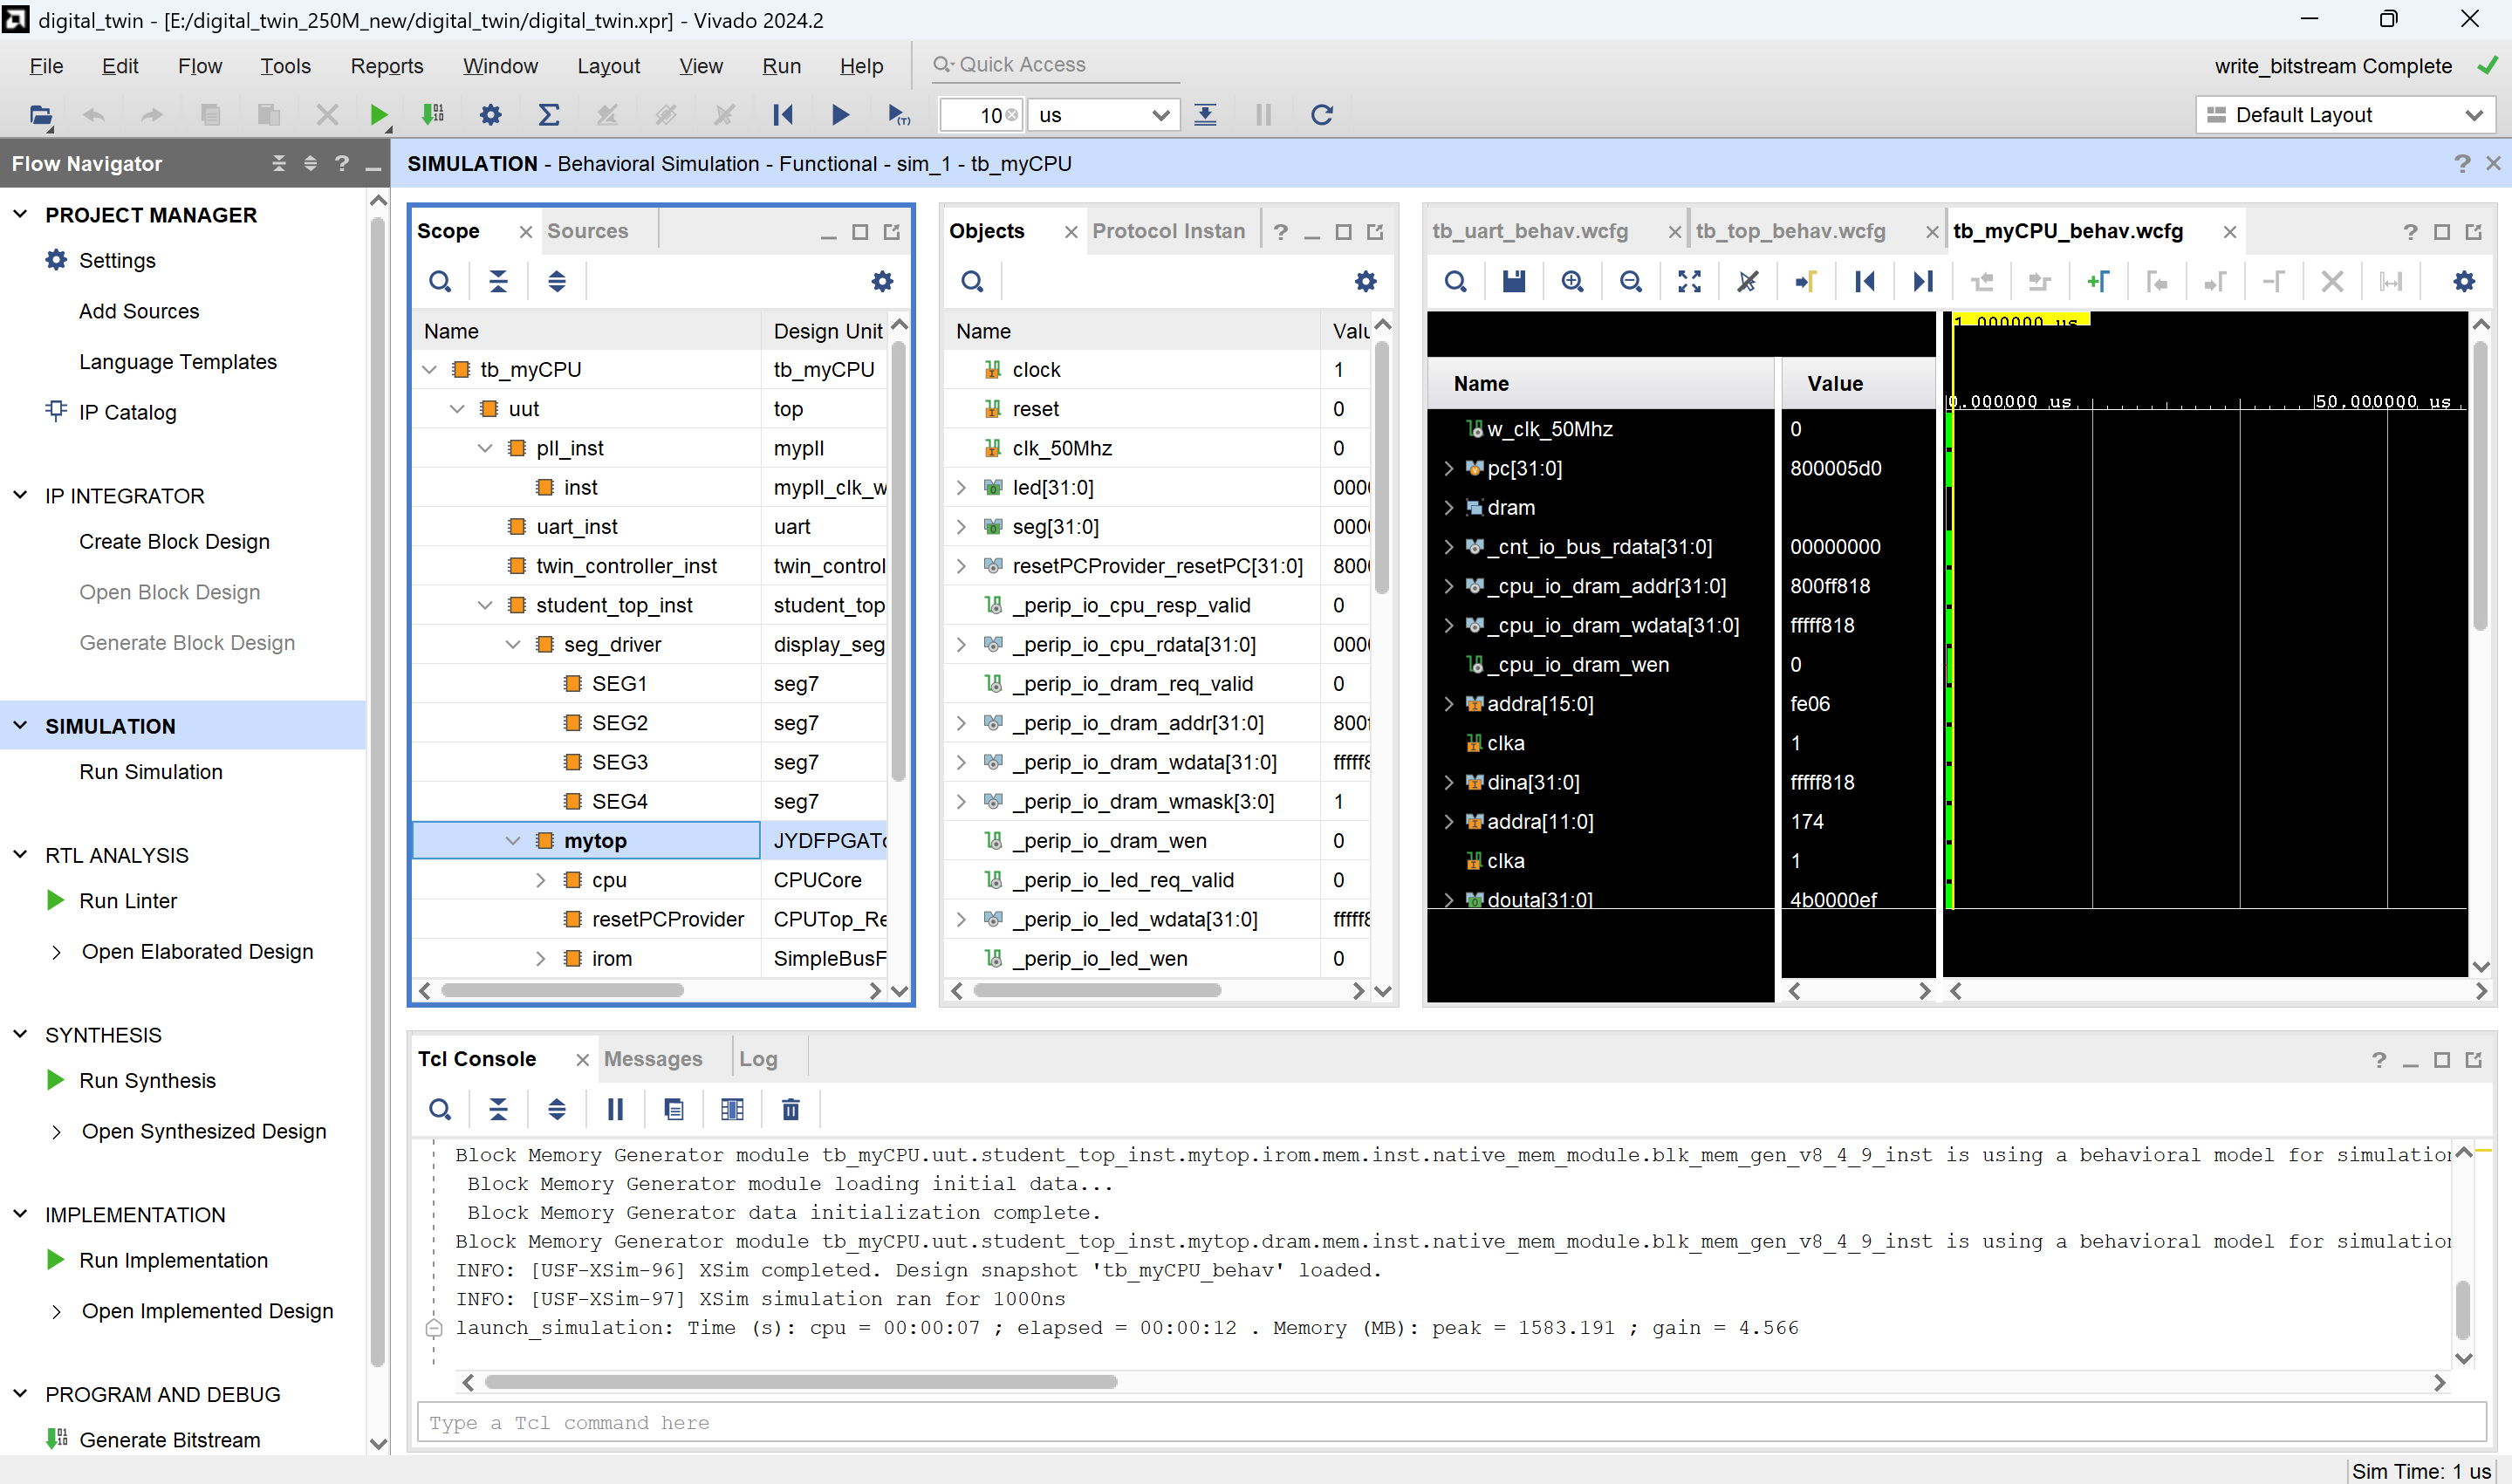
\includegraphics[width=0.95\linewidth]{verify/image8.png}
  \caption{Vivado Simulation 仿真工程界面}
\end{figure}

\subsubsection{Verilator 与 NEMU 差分验证}

SystemVerilog 由 Verilator 编译为周期级仿真器。仿真器在指令提交边界将 DUT 的 PC、通用寄存器与
相关体系结构状态同 NEMU 参考模型比较；发生不一致时输出最近指令环、寄存器和访存上下文。DPI-C
同时承担 EBREAK 停机识别、串口模拟、外设行为和性能计数采集。该平台能够快速运行单指令测试、
CPU tests、体系结构测试和完整性能负载。

仿真器中的 Perf Counters Report 统计周期数、提交指令数、IPC、CPI、分支预测准确率和 RAW stall
等指标。测试程序结束时执行 EBREAK，仿真器读取返回寄存器并判定 good trap；对赛题 COE，则先转换
为仿真可加载的 IROM/DRAM 镜像，再运行至设备输出或停机条件。

\begin{figure}[H]
  \centering
  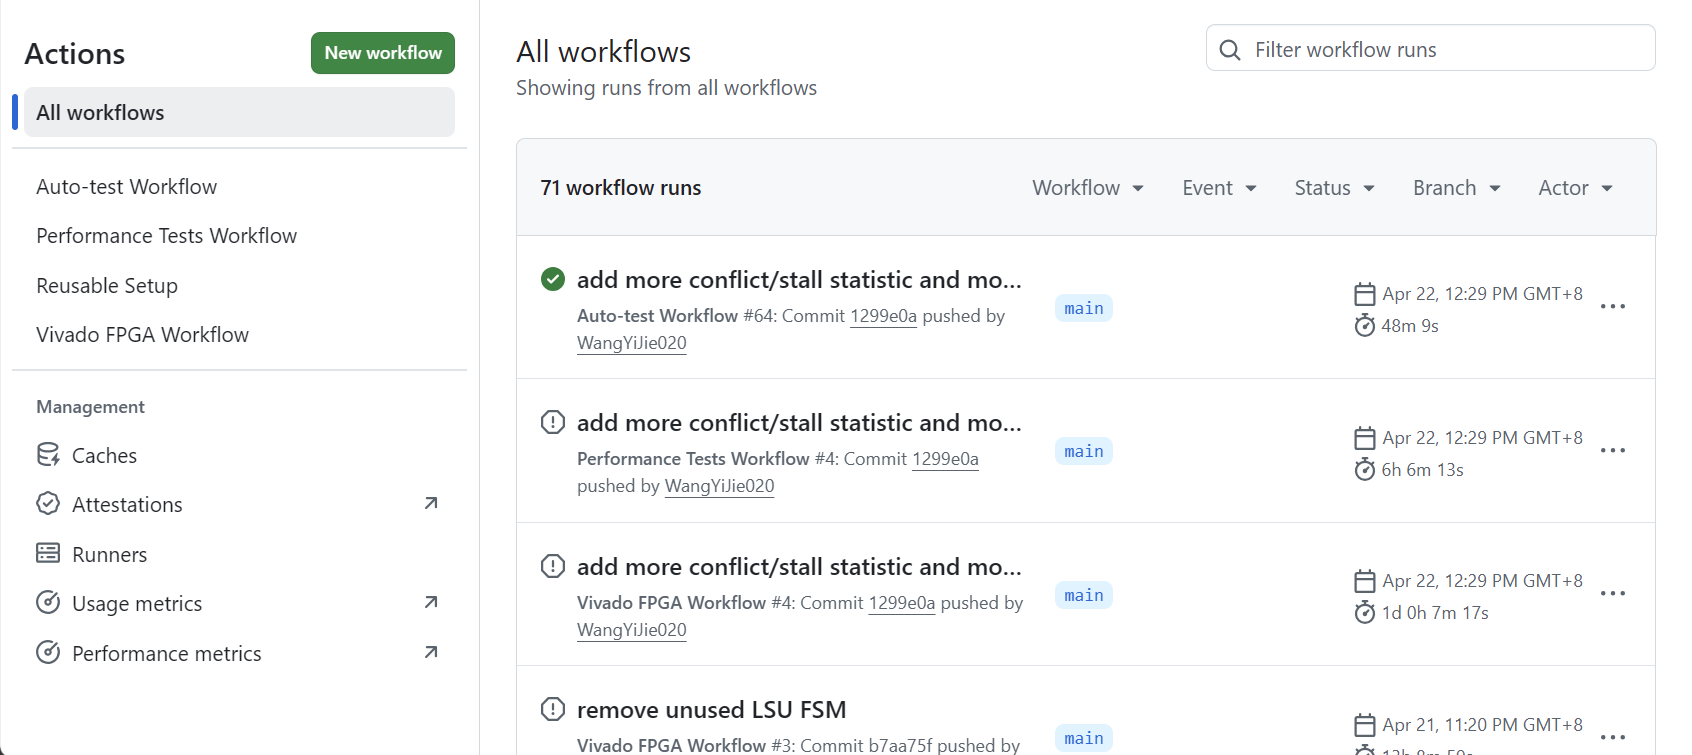
\includegraphics[width=0.95\linewidth]{verify/image9.png}
  \caption{自动化回归与实现流程界面}
\end{figure}

\subsubsection{FPGA 实现与板测}

目标平台采用 Xilinx Kintex-7 XC7K325T-2FFG900 和 Vivado 2024.2。实现流程重新生成并打包
SystemVerilog，刷新工程输入，完成 synthesis、implementation、bitstream 和时序报告提取。板测通过
自动化 capture 保存原始 UART 输出；正式记录包含板卡、CPU 频率、程序镜像、bitstream 身份、CRC、
硬件计时值与完整串口文本。LED 和数码管仍用于快速观察外设写入，UART 则用于保留可解析的量化证据。

\subsection{测试用例与自动化流程}

\subsubsection{基础指令与小程序}

基础测试同时采用单指令边界用例和小规模程序。单指令测试覆盖算术、逻辑、移位、比较、分支、跳转、
load/store 以及 RV32M 和已实现扩展；程序级测试覆盖 add、load-store、switch、if-else、recursion
等常见组合。测试资源包括移植到 AbstractMachine 的 riscv-tests、riscv-arch-test，以及
am-kernels/tests/cpu-tests。

\begin{figure}[H]
  \centering
  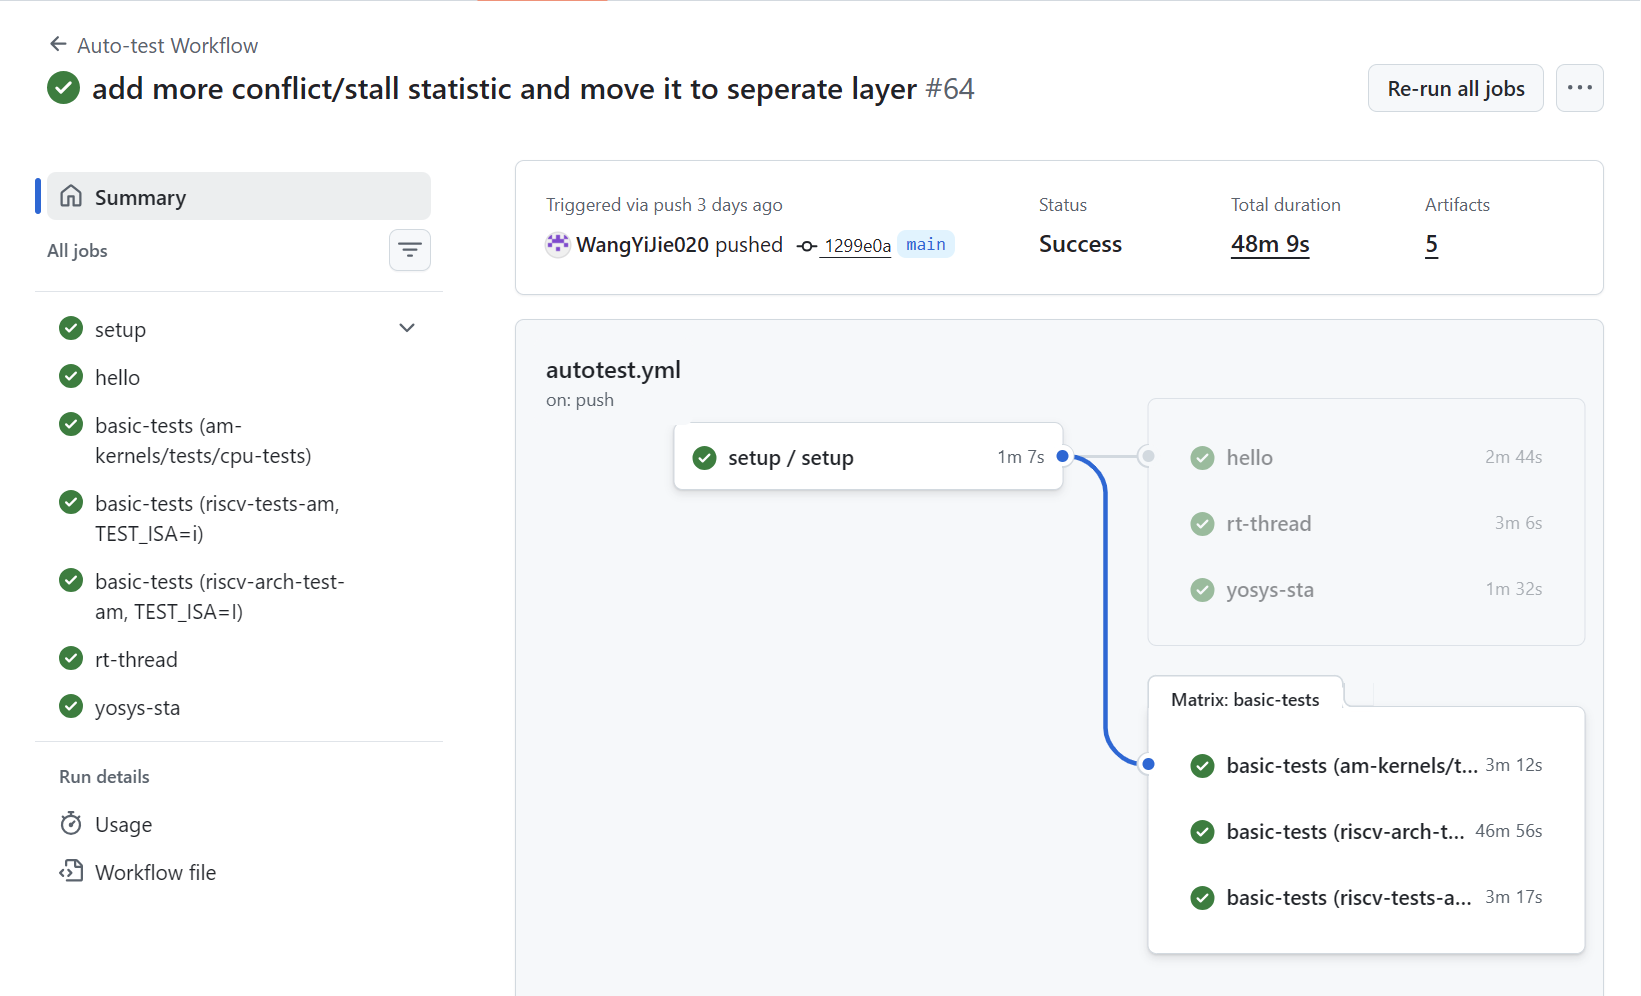
\includegraphics[width=0.92\linewidth]{verify/image10.png}
  \caption{基础正确性测试自动化流程}
\end{figure}

\subsubsection{性能与系统负载}

性能测试保留赛题提供的 src0、src1、src2、withoutMext 与 withMext，并使用 CoreMark、Dhrystone
和总决赛正式性能负载进行回归。仿真阶段记录总周期和提交指令数，按实际目标频率换算时间；板测阶段
以硬件计时器与 UART 原始输出为准。只有结果校验和 CRC 均正确时，时间数据才进入性能表和折线图。

\begin{figure}[H]
  \centering
  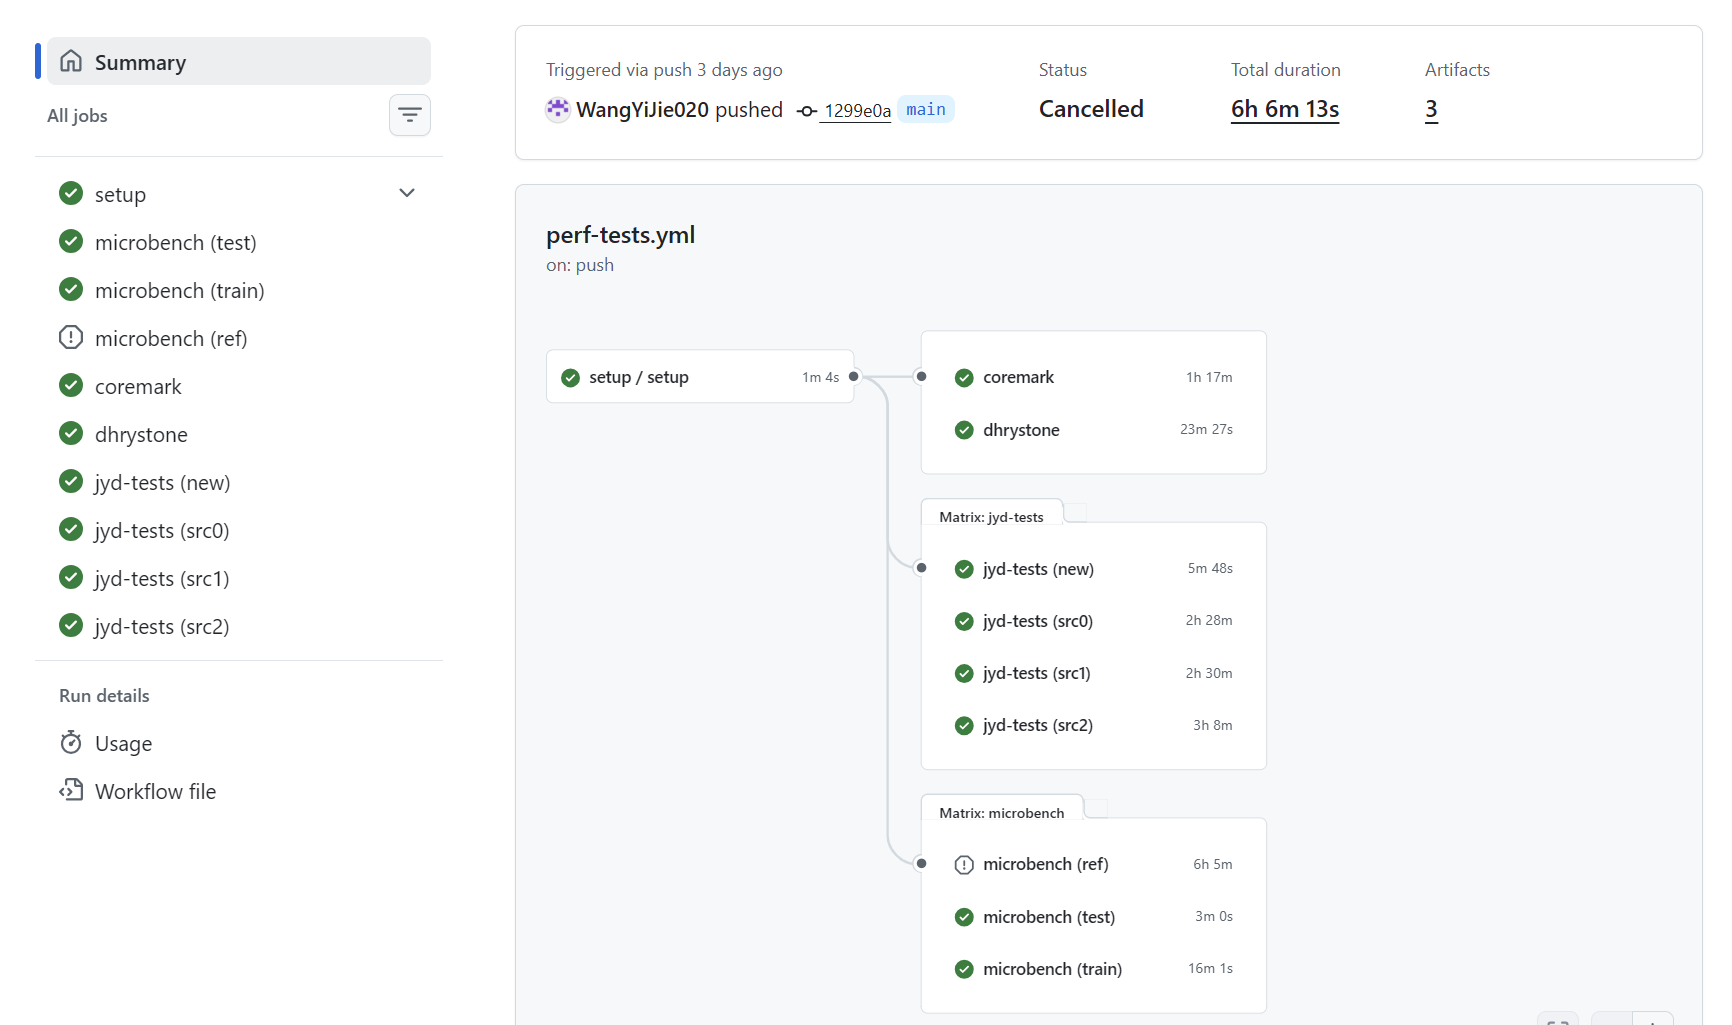
\includegraphics[width=0.95\linewidth]{verify/image11.png}
  \caption{性能测试自动化流程}
\end{figure}

\subsubsection{CSR、机器态与 RT-Thread}

CSR 测试覆盖 \texttt{mcycle(h)}、\texttt{mstatus}、\texttt{mepc}、\texttt{mtvec}、
\texttt{marchid}、\texttt{mvendorid} 以及 CSR 读改写、\texttt{ecall} 和 \texttt{mret}。
RT-Thread 测试进一步组合上下文切换、异常返回、串口输入、内存分配和命令执行；仿真到达
\texttt{msh />} 提示符后，继续运行 version、free、hello、microbench 与 echo 等命令。

\subsection{分层覆盖与专项检查}

\begin{table}[H]\centering
\caption{验证层次、主要内容与判定标准}
\small
\begin{tabularx}{\linewidth}{@{}p{0.18\linewidth}YY@{}}
\toprule
\textbf{测试层次}&\textbf{主要内容}&\textbf{判定标准}\\\midrule
基础 CPU tests&add、load-store、switch、if-else、recursion&程序 good trap，差分无不一致\\
RV32I/M 架构测试&整数、分支、访存、乘除法及边界条件&体系结构签名通过，RAW 停顿正确\\
CSR/机器态测试&CSR 读改写、ecall、mret、RT-Thread&状态更新正确，可进入 shell 并执行命令\\
B 扩展测试&各已实现短操作与迭代操作&指令结果及边界行为与参考语义一致\\
自定义指令测试&单周期、状态型、访存型和归约型单元&返回值、内部状态、访存副作用符合指令语义\\
完整性能负载&固定镜像和正式迭代次数&全部 CRC 正确，周期与板测记录完整\\
Vivado Sim.&存储 IP、SEG/LED、UART 与顶层接口&波形和设备输出符合接口时序\\
Vivado 实现&setup/hold、DRC、unrouted nets&报告阶段和频率明确，无硬错误\\
真实板测&相同 bitstream 的多次 capture&每次 CRC 正确，时间重复性可解释\\
\bottomrule
\end{tabularx}
\end{table}

\subsubsection{RAW、旁路与多周期执行}

专项用例覆盖立即消费、隔一条消费、两个源寄存器同时相关、后级反压、多周期完成同拍消费和提交阻塞。
生产者在数据尚未有效时保留目的寄存器占用，使 IDU 停顿；结果有效后才解除停顿或进入专用旁路。
相邻快速结果 token 只服务规定的消费者，不进入地址、多周期、CSR 或自定义指令通路。

\subsubsection{load-use、控制流与缓存一致性}

命中路径检查 LB/LBU/LH/LHU/LW 的地址低位与扩展结果，miss 路径检查响应捕获、回填和消费者恢复。
BEQ/BNE 的 late-load 比较覆盖预测正确与错误，确保重定向只发生一次，较年轻指令及其访存副作用均被
抑制。缓存专项场景包括 load fill、整字 store 分配、窄 store 失效、store 与旧 load 回填竞争、双
bank 连续访问、同步 BRAM bank 对齐，以及自定义访存单元产生的缓存更新。

\subsection{代表性验证结果}

\subsubsection{RV32I 基本指令测试}

\begin{figure}[H]
  \centering
  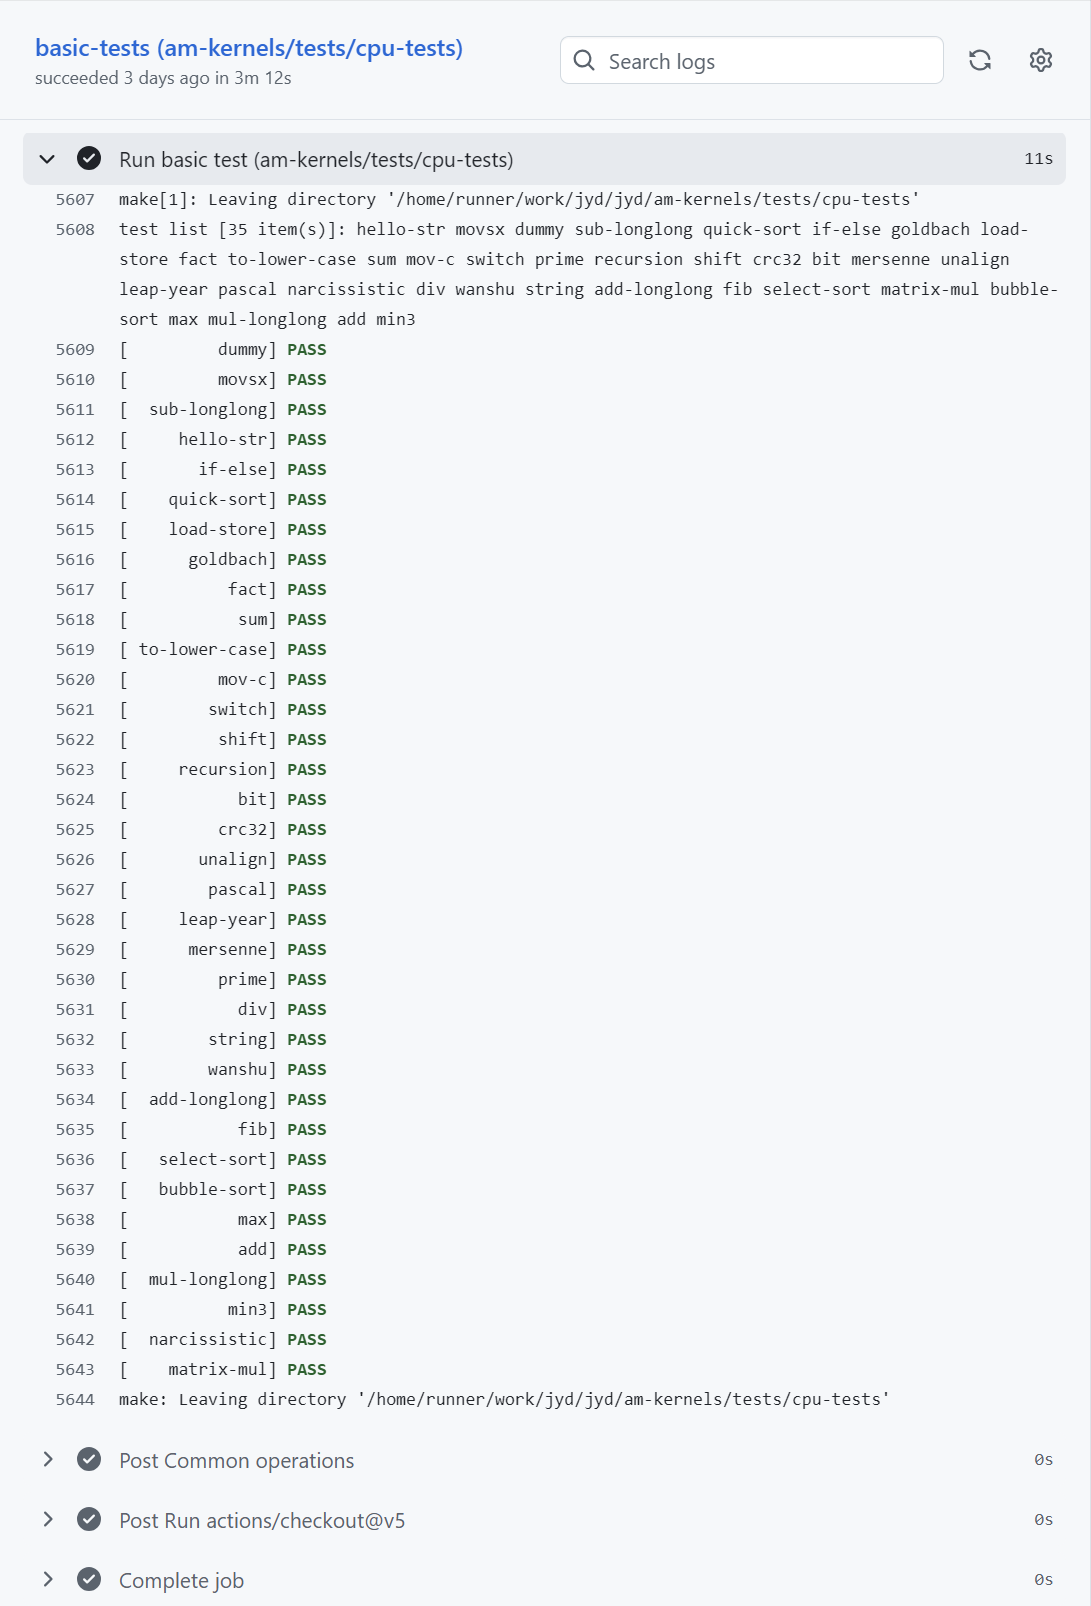
\includegraphics[height=0.58\textheight,trim=0 0 669bp 0,clip]{verify/image13.png}%
  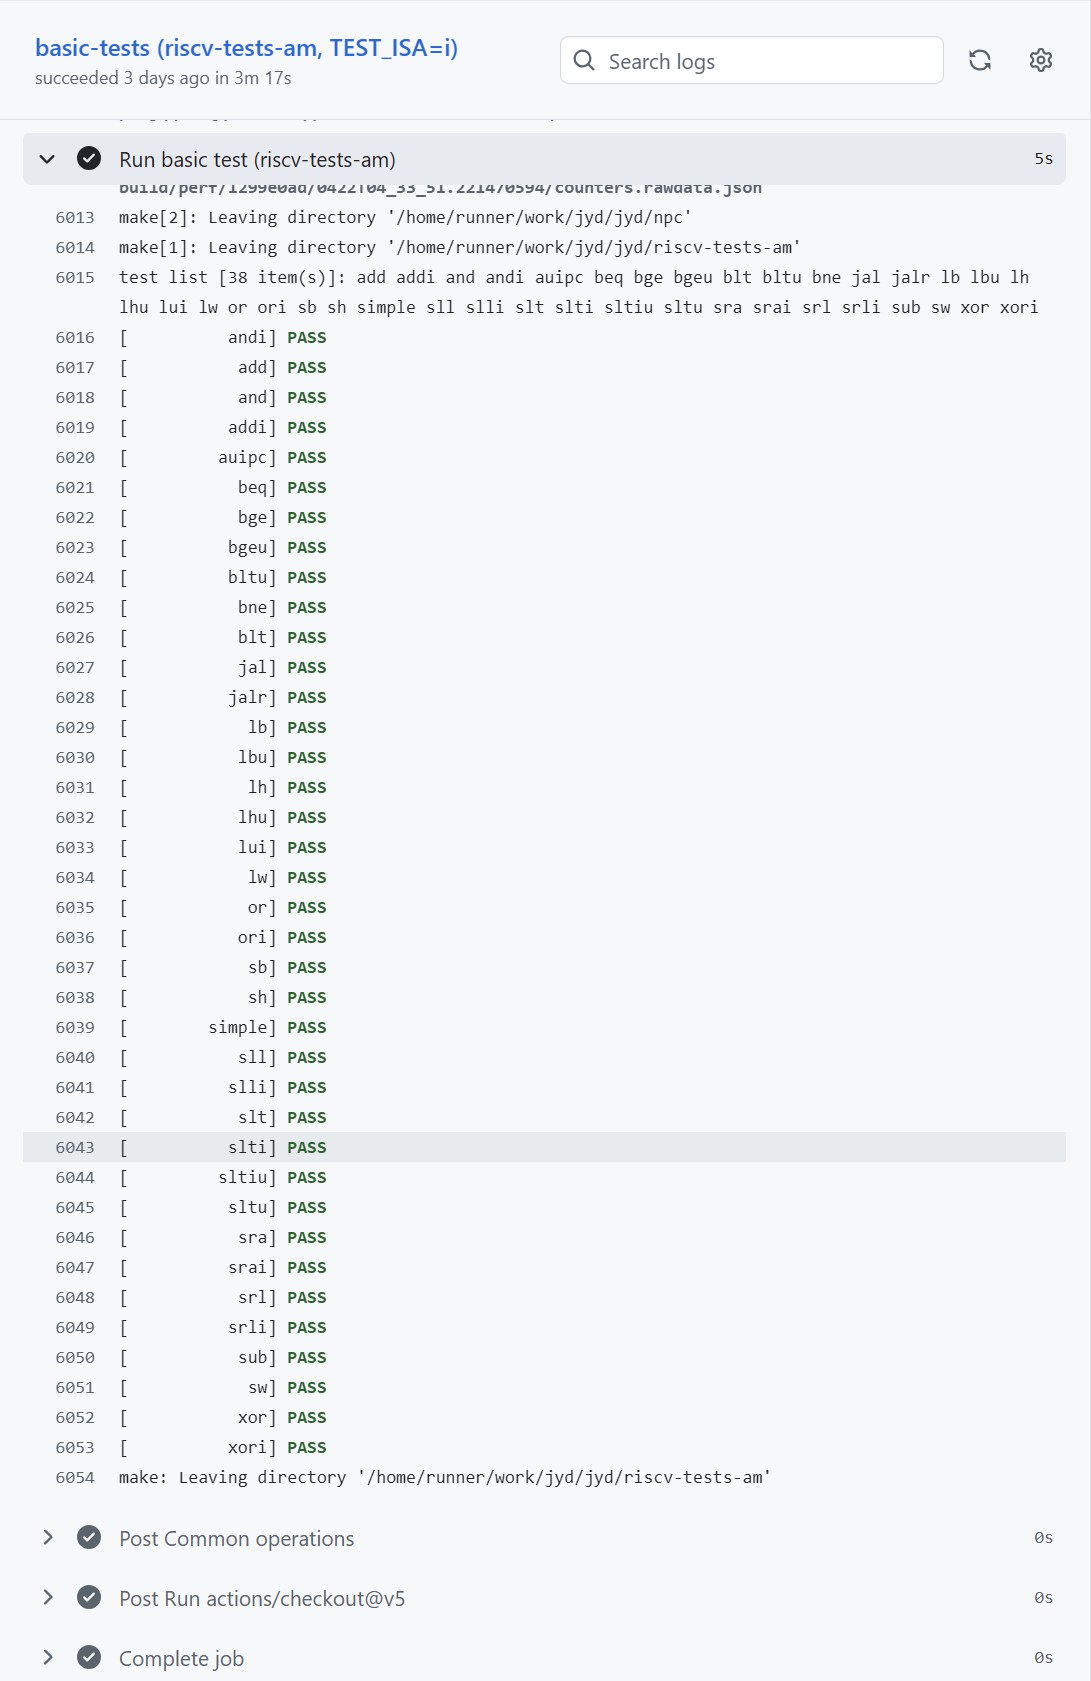
\includegraphics[height=0.58\textheight,trim=0 0 644bp 0,clip]{verify/image14.png}%
  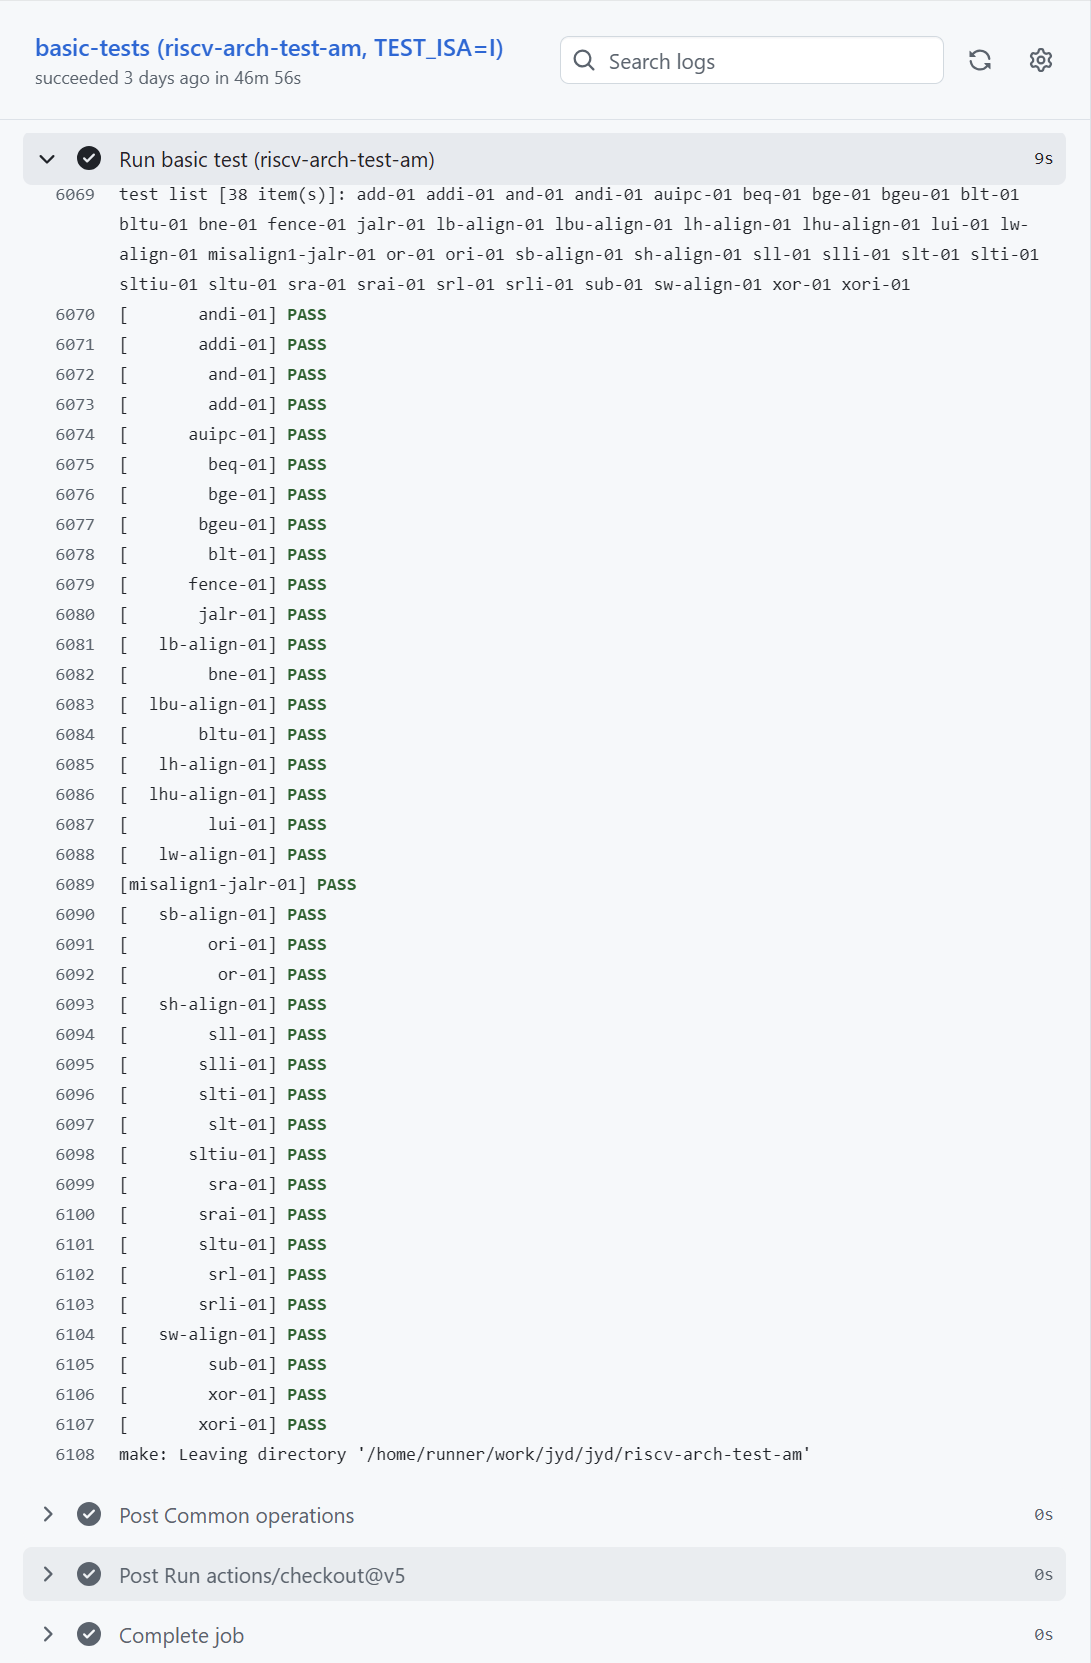
\includegraphics[height=0.58\textheight,trim=0 0 654bp 0,clip]{verify/image15.png}
  \caption{RV32I 基本指令测试结果}
\end{figure}

单指令与边界样例全部通过，程序以 good trap 结束。该组回归覆盖 RV32I 算术逻辑、移位、比较、
跳转、分支和访存路径，是后续缓存、预测器与执行通路迭代的基础门禁。

\subsubsection{src0、src1 与 src2 性能测试}

\begin{figure}[H]
  \centering
  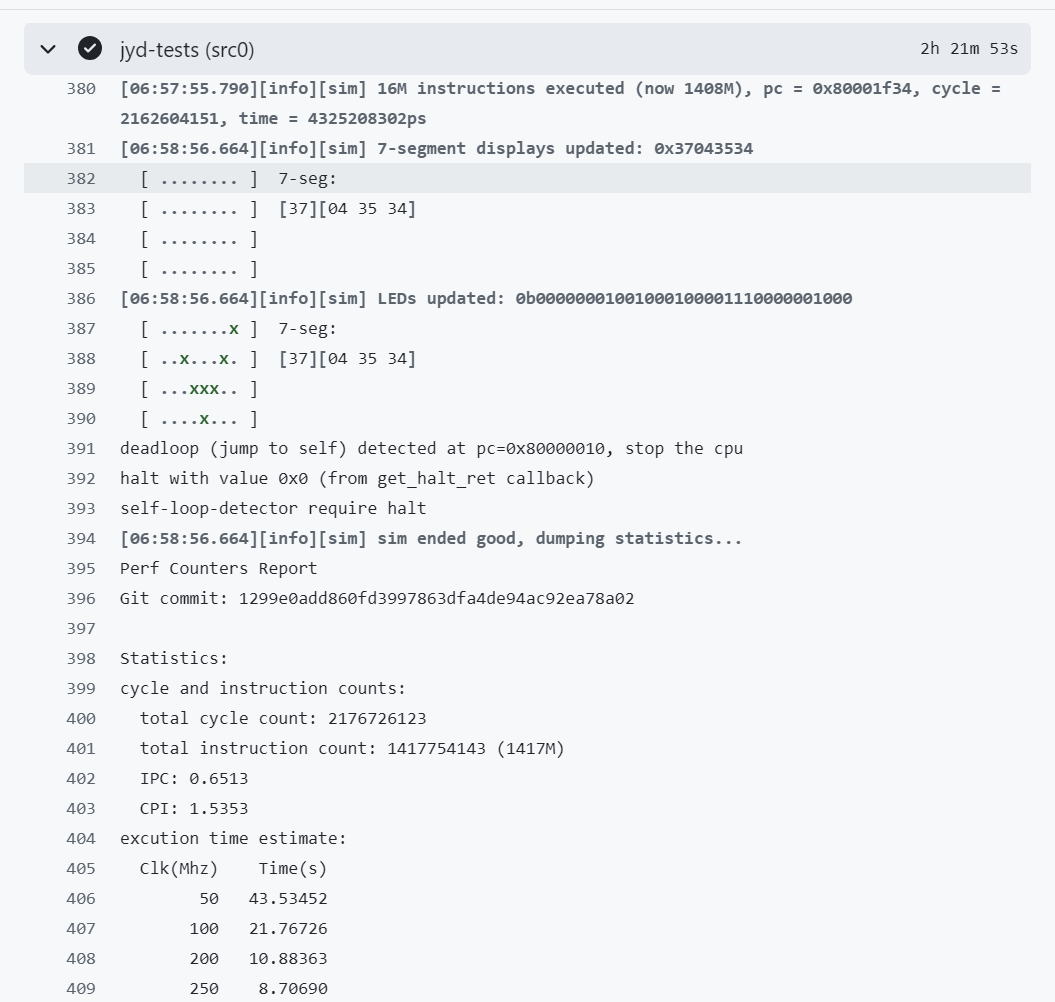
\includegraphics[width=0.82\linewidth,trim=0 365bp 0 0,clip]{verify/image16.png}
  \caption{src0 仿真日志与性能统计}
\end{figure}

src0 完成 37 条功能测试并进入 halt。分赛区阶段记录为 1,988,372,516 周期、1,417M 条动态指令，
IPC 0.7130、CPI 1.4025；按 280\,MHz 计算为 7.10133\,s，与当时板测显示一致。

\begin{figure}[H]
  \centering
  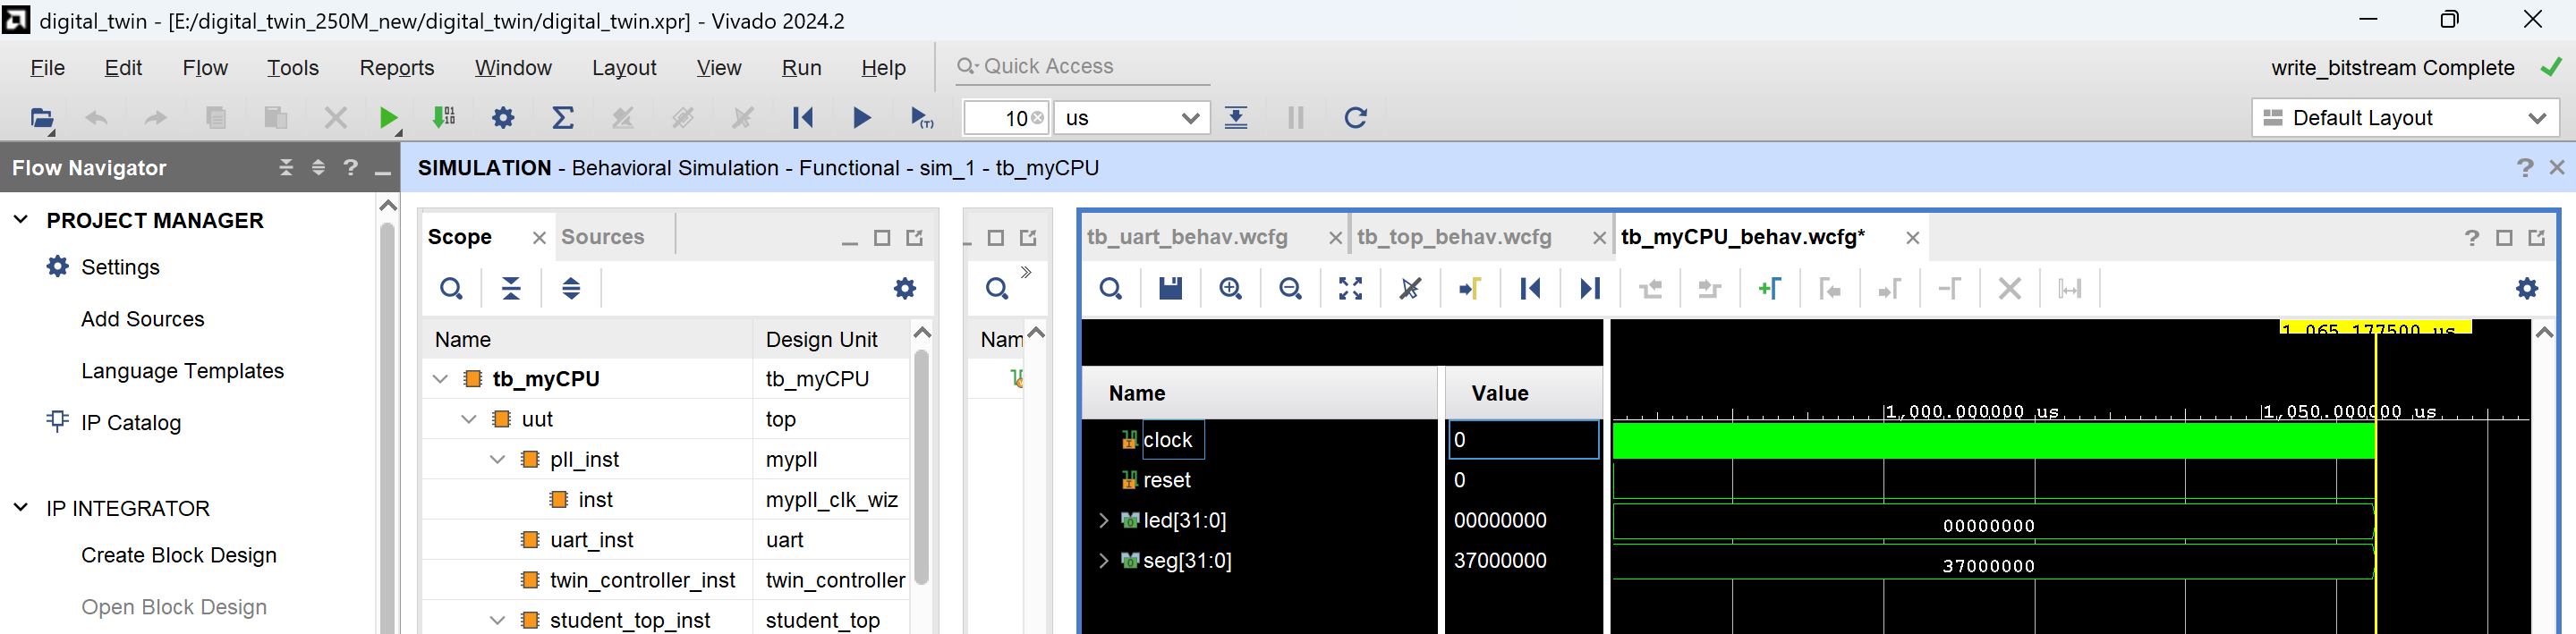
\includegraphics[width=\linewidth]{verify/image17.png}
  \caption{src0 Vivado Simulation 波形}
\end{figure}

\begin{figure}[H]
  \centering
  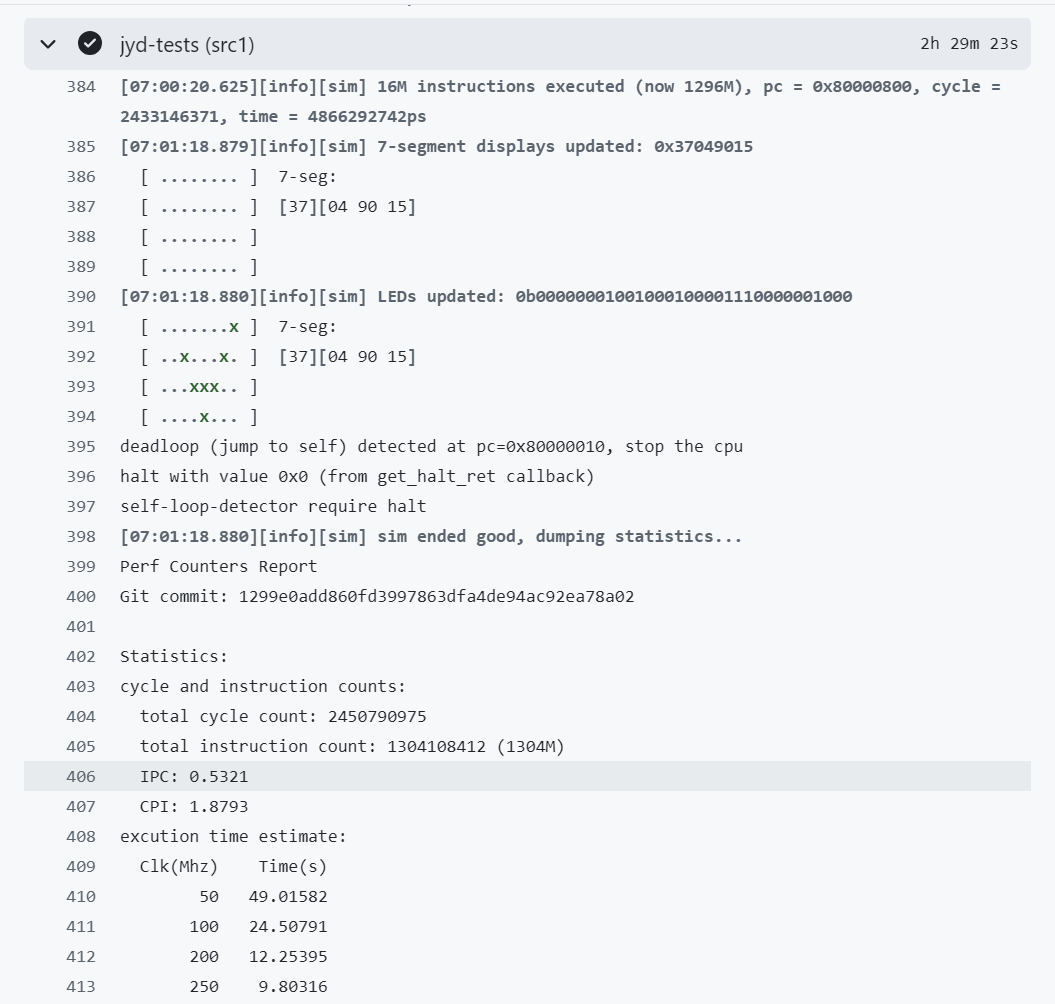
\includegraphics[width=0.82\linewidth,trim=0 350bp 0 0,clip]{verify/image18.png}
  \caption{src1 仿真日志与性能统计}
\end{figure}

src1 记录为 1,973,306,668 周期、1,304M 条动态指令，IPC 0.6609、CPI 1.5131；280\,MHz 换算
时间为 7.04752\,s。对应 Vivado Simulation 波形中，数码管写入 37000000，表明 37 条功能测试完成。

\begin{figure}[H]
  \centering
  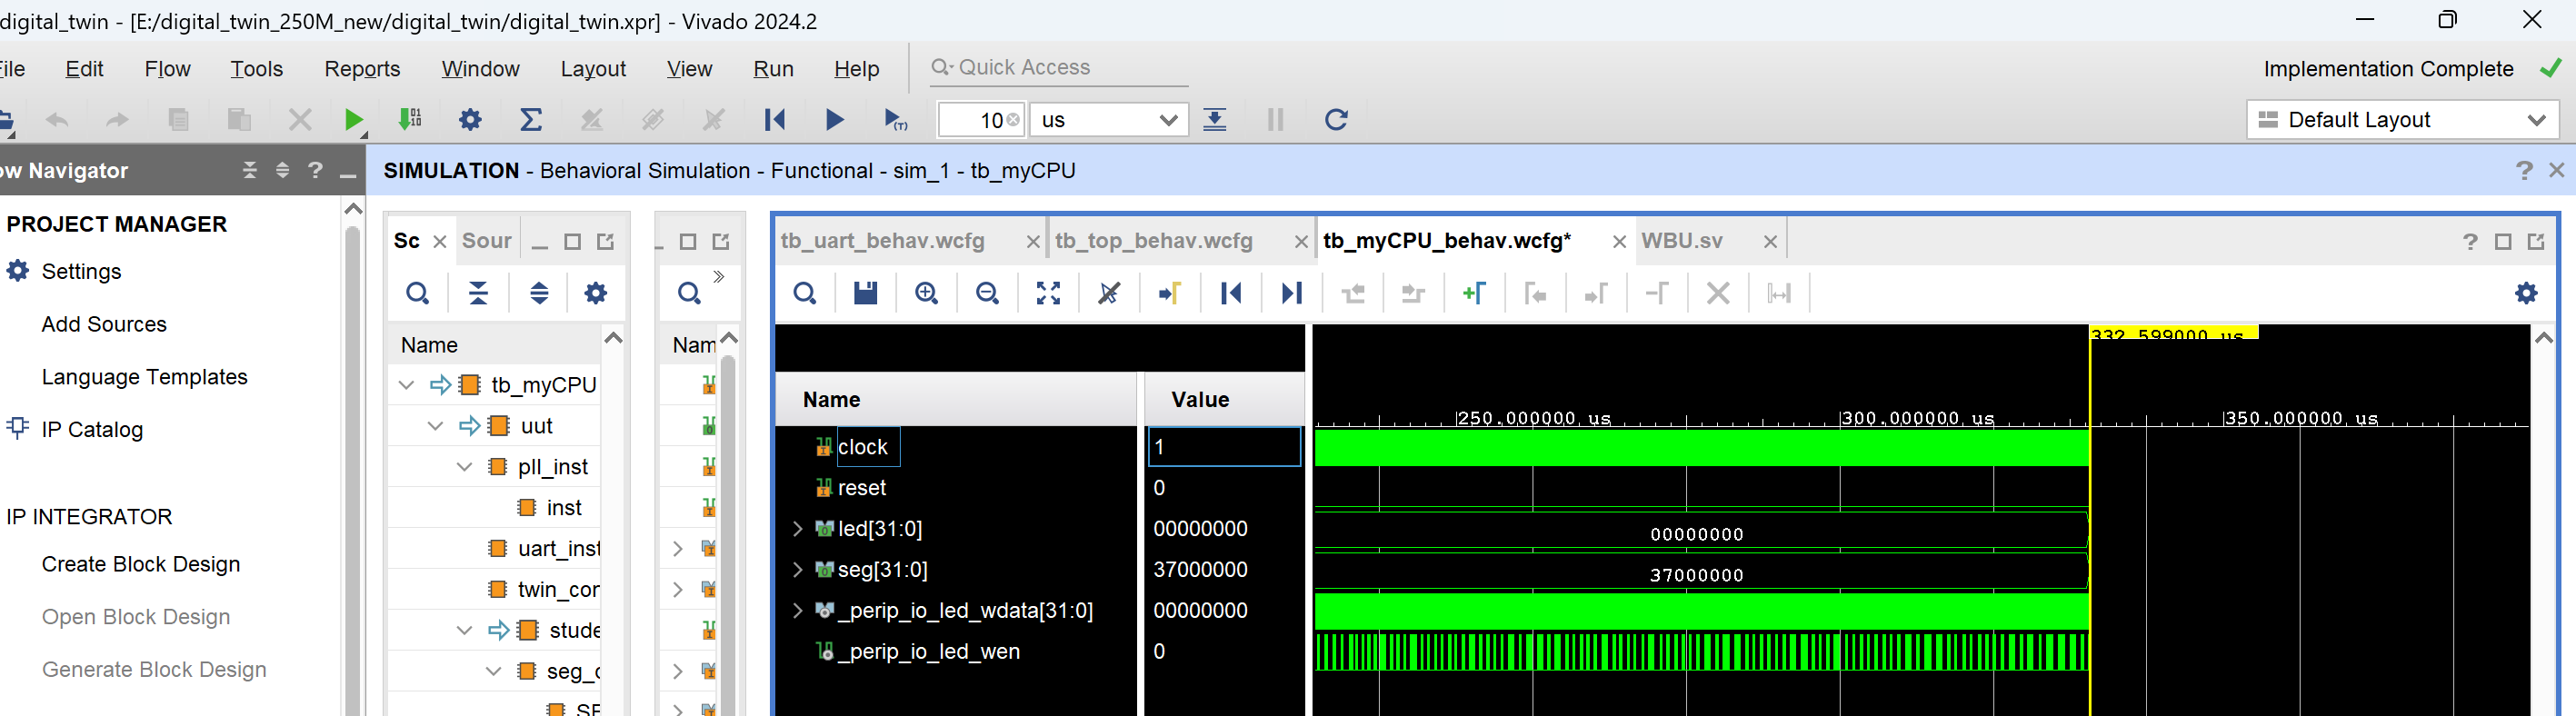
\includegraphics[width=\linewidth]{verify/image19.png}
  \caption{src1 Vivado Simulation 波形}
\end{figure}

\begin{figure}[H]
  \centering
  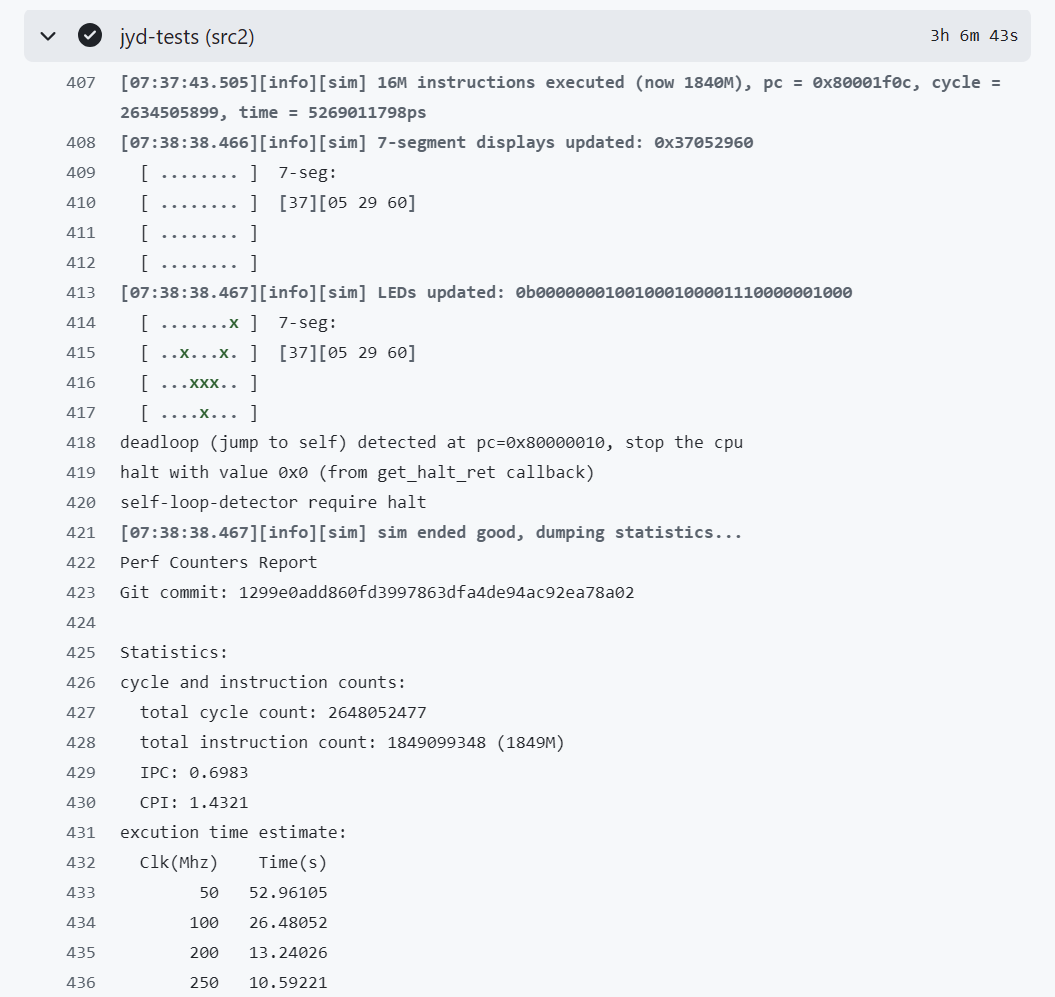
\includegraphics[width=0.82\linewidth,trim=0 340bp 0 0,clip]{verify/image20.png}
  \caption{src2 仿真日志与性能统计}
\end{figure}

src2 记录为 2,585,374,792 周期、1,849M 条动态指令，IPC 0.7152、CPI 1.3982；280\,MHz 换算
时间为 9.23348\,s。其 Vivado Simulation 波形同样完成数码管结果写入。

\begin{figure}[H]
  \centering
  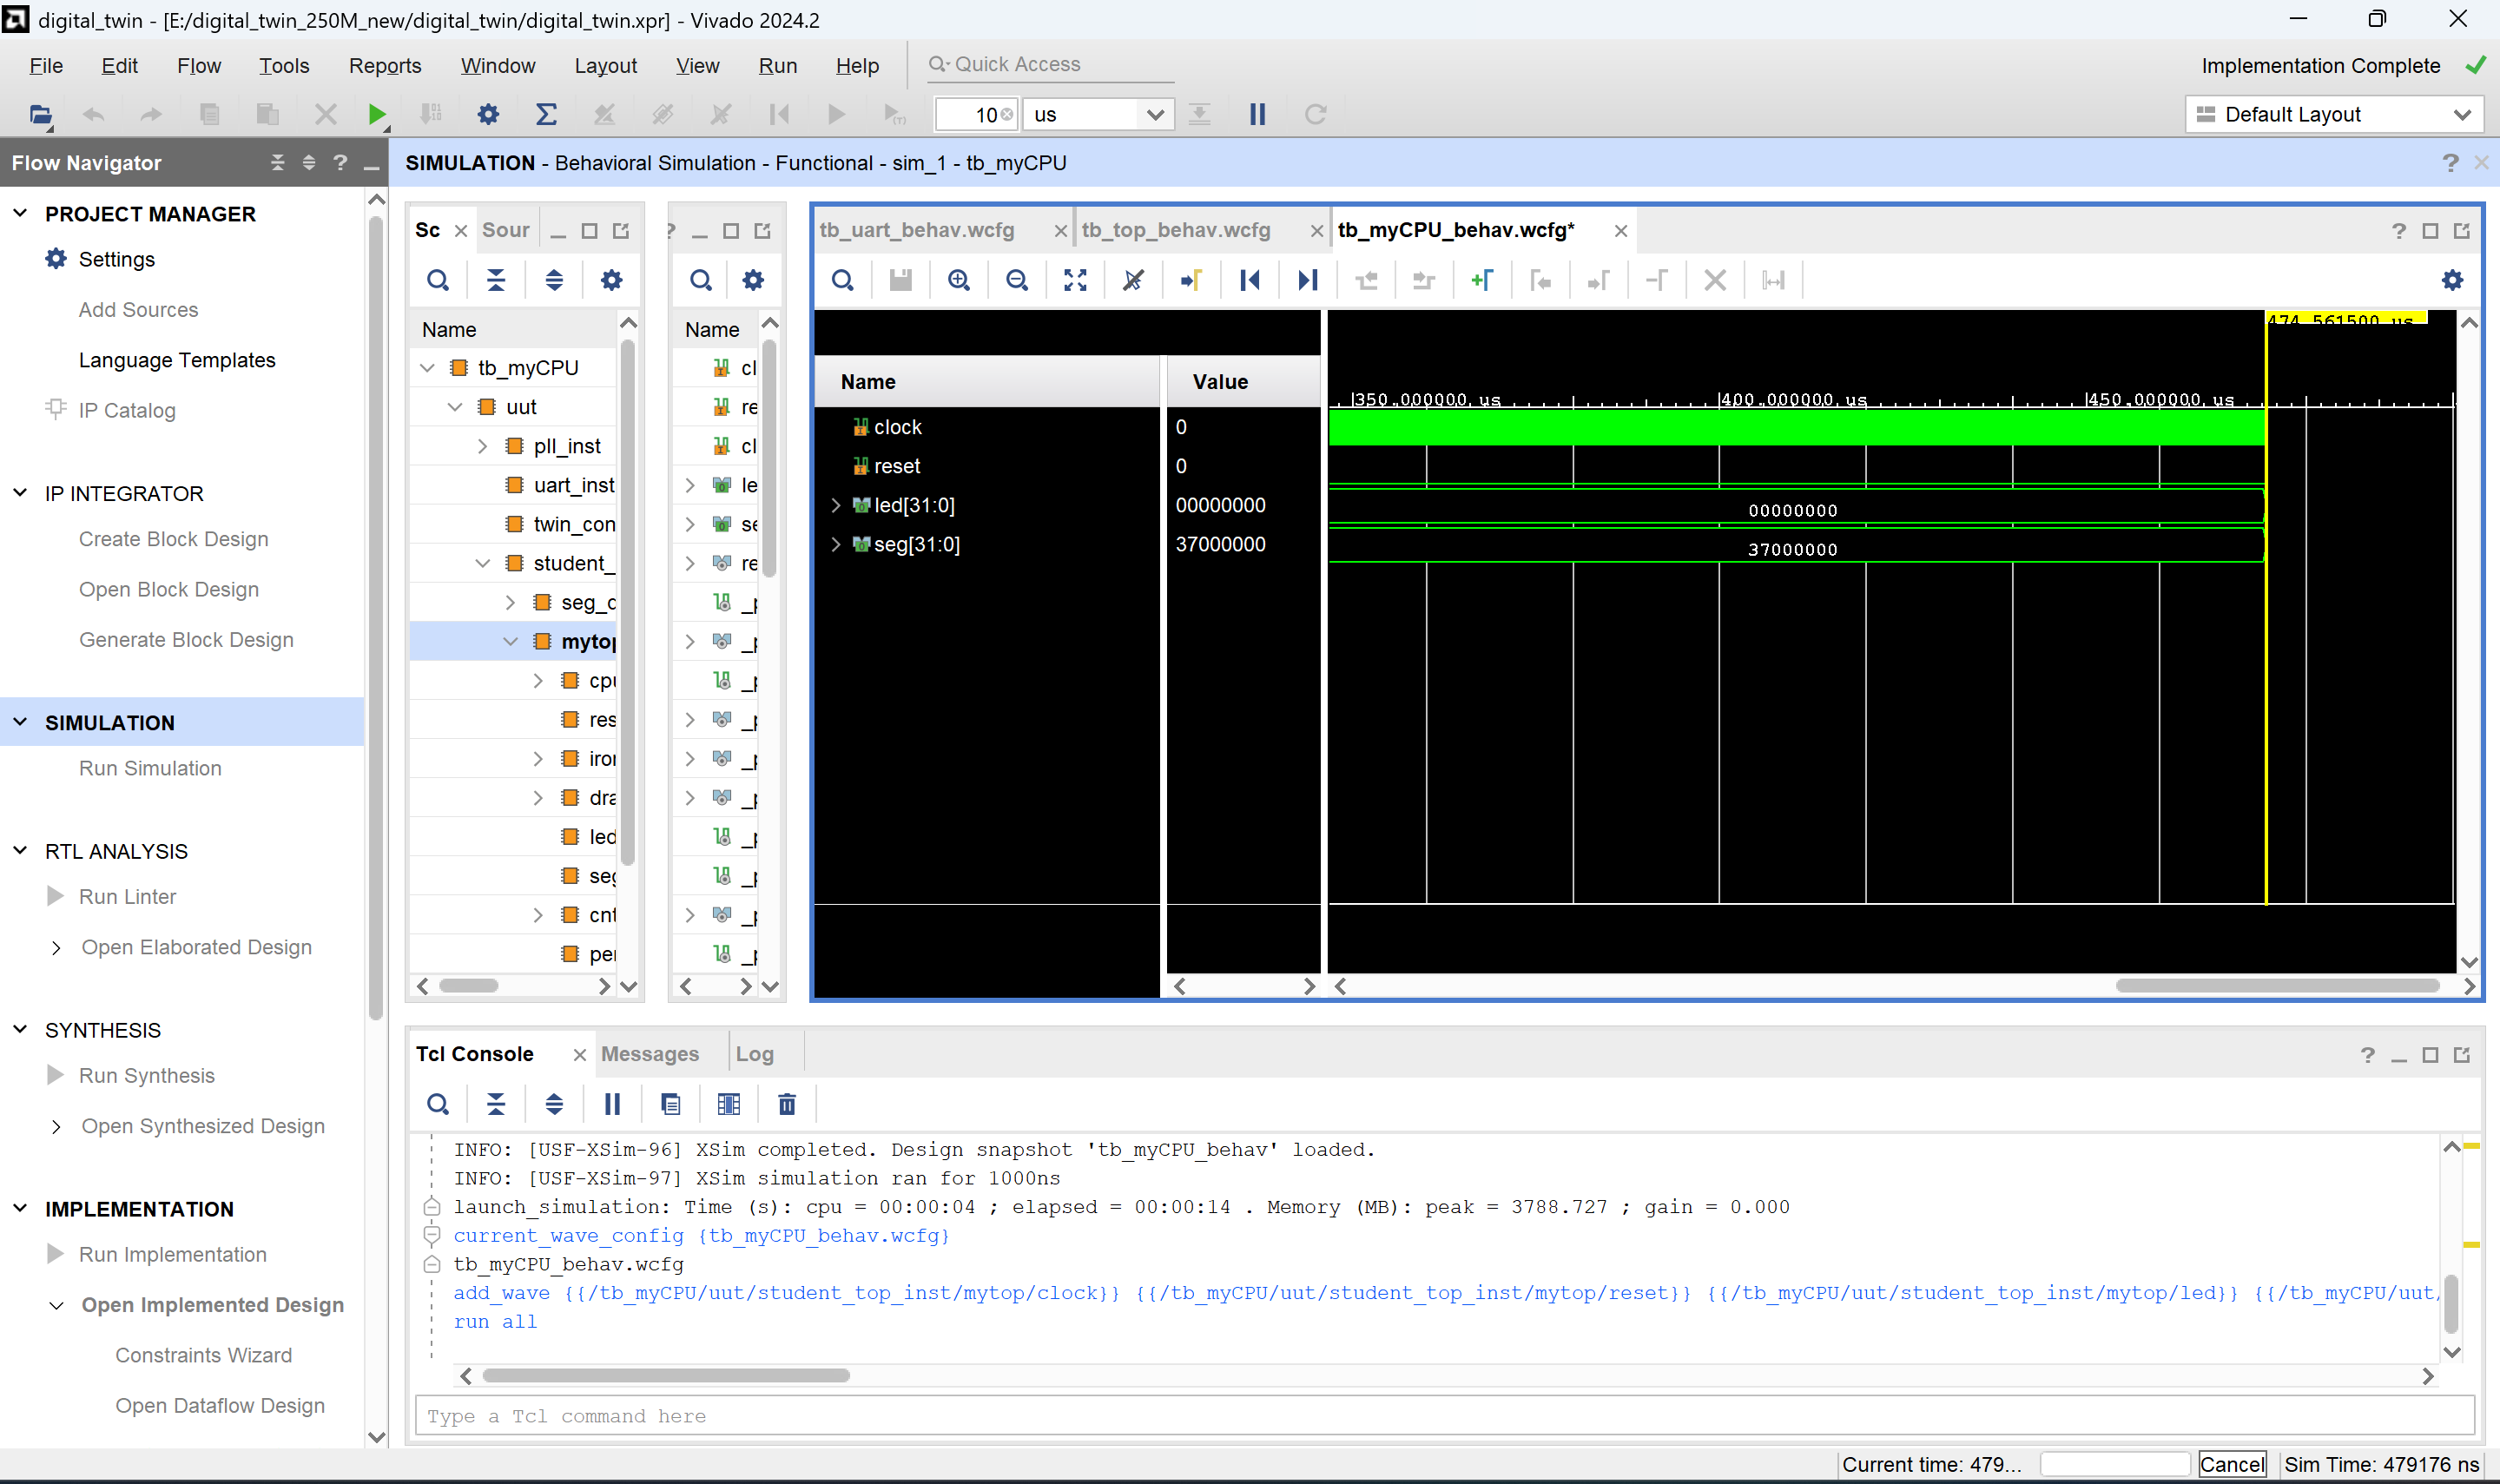
\includegraphics[width=\linewidth]{verify/image21.png}
  \caption{src2 Vivado Simulation 波形}
\end{figure}

\begin{table}[H]\centering
\caption{src0、src1、src2 性能统计结果}
\small
\begin{tabularx}{\linewidth}{@{}lrrrrr@{}}\toprule
\textbf{用例}&\textbf{周期数}&\textbf{指令数}&\textbf{IPC}&\textbf{CPI}&\textbf{280 MHz 时间/s}\\\midrule
src0&1988M&1417M&0.7130&1.4025&7.10133\\
src1&1973M&1304M&0.6609&1.5131&7.04752\\
src2&2585M&1849M&0.7152&1.3982&9.23348\\
\bottomrule\end{tabularx}
\end{table}

\subsubsection{CoreMark 与 Dhrystone}

\begin{figure}[H]
  \centering
  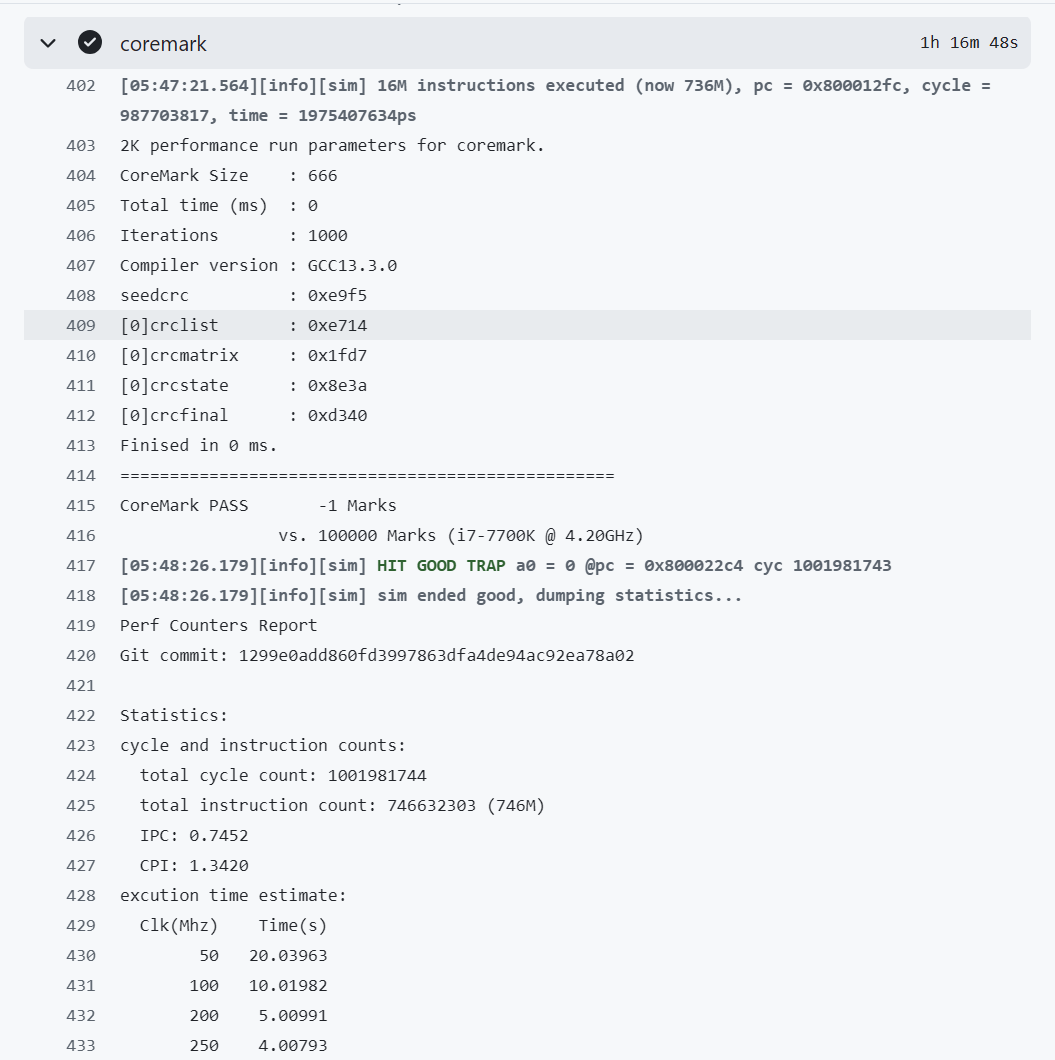
\includegraphics[width=0.82\linewidth,trim=0 440bp 0 0,clip]{verify/image22.png}
  \caption{CoreMark 测试结果}
\end{figure}

分赛区阶段 1000 次 CoreMark 迭代共执行 472,993,621 周期，IPC 0.6625、CPI 1.5094；按
280\,MHz 计算运行时间为 1.68926\,s，对应 CoreMark 308、CoreMark/MHz 1.10。总决赛正式负载
进一步以 10000 次迭代和四项 CRC 作为板测判据，其完整性能演进见第\ref{sec:performance}节。

\begin{figure}[H]
  \centering
  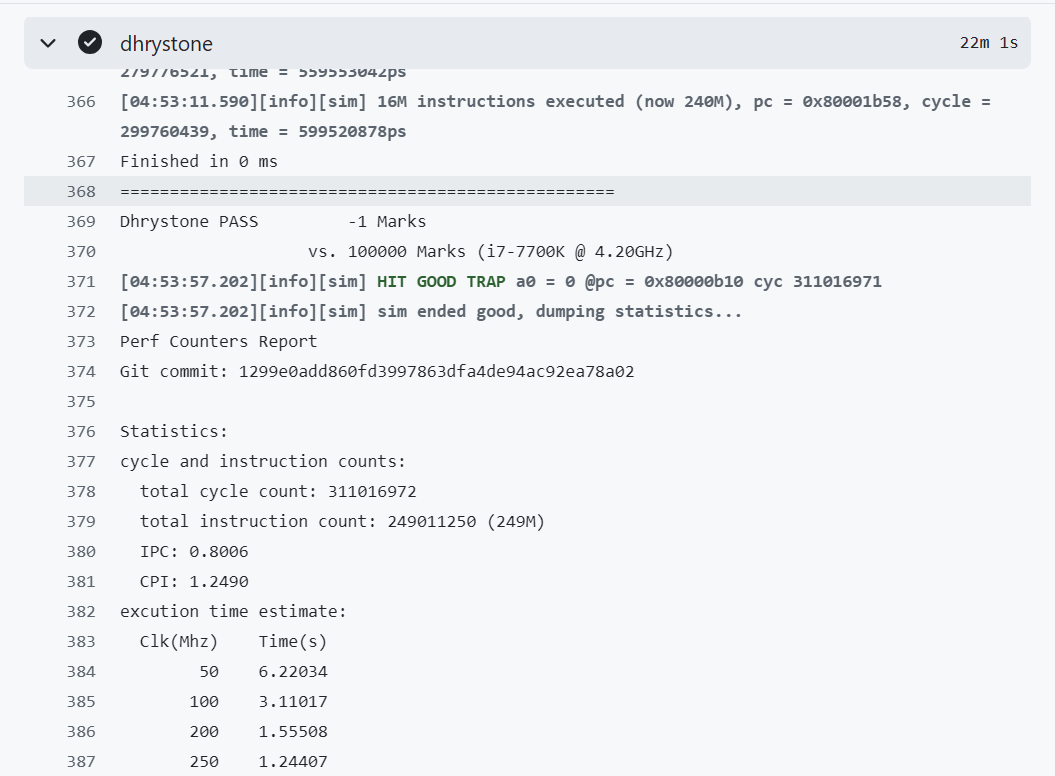
\includegraphics[width=0.82\linewidth,trim=0 545bp 0 0,clip]{verify/image23.png}
  \caption{Dhrystone 测试结果}
\end{figure}

Dhrystone 500000 次迭代执行 302,517,149 周期，IPC 0.7768、CPI 1.2873；按 280\,MHz 计算为
1.08042\,s，对应约 462,784 Dhrystones/s、263.39 DMIPS 和 0.941 DMIPS/MHz。

\subsubsection{RT-Thread 系统测试}

\begin{figure}[H]
  \centering
  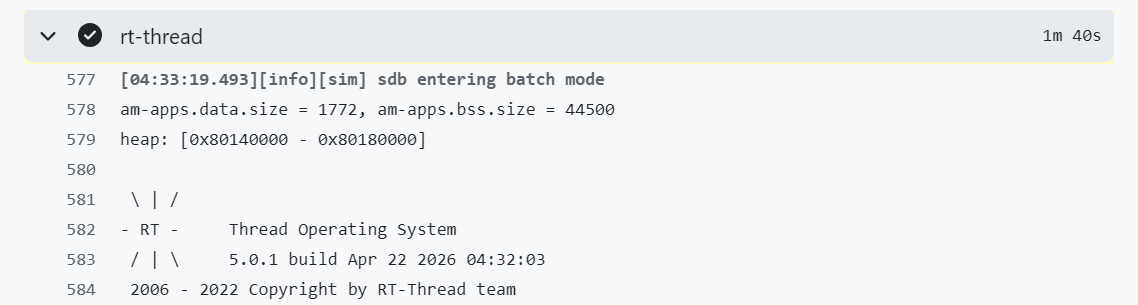
\includegraphics[width=0.9\linewidth]{verify/image12.png}
  \caption{RT-Thread 启动与 shell 提示符}
\end{figure}

\begin{figure}[H]
  \centering
  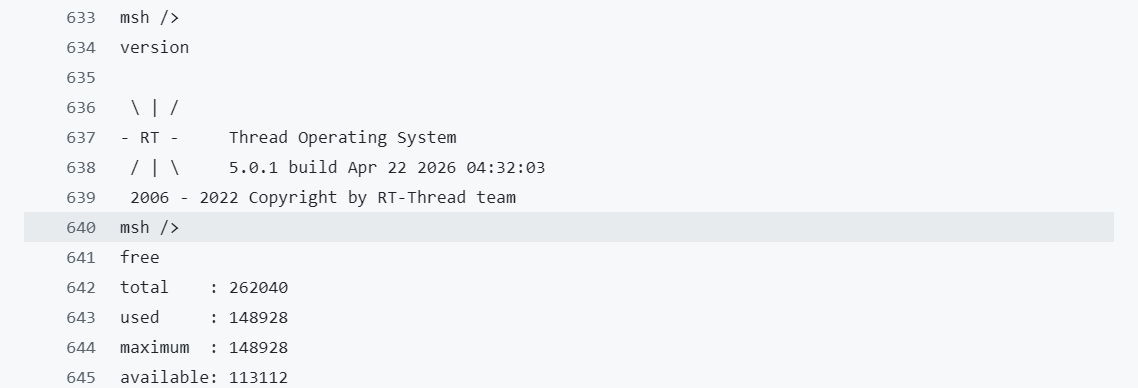
\includegraphics[width=\linewidth]{verify/image24.png}
  \vspace{0.25em}
  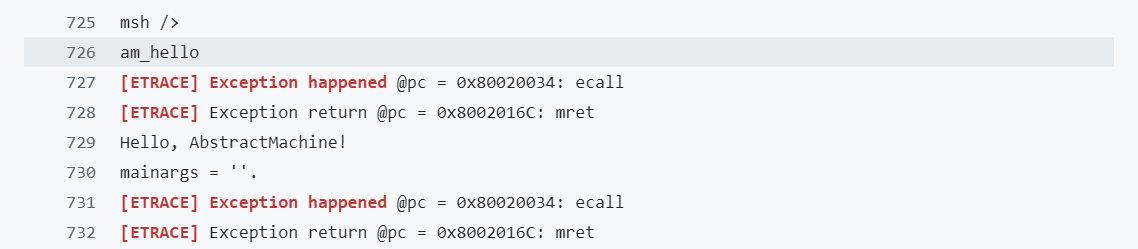
\includegraphics[width=\linewidth]{verify/image25.png}
  \vspace{0.25em}
  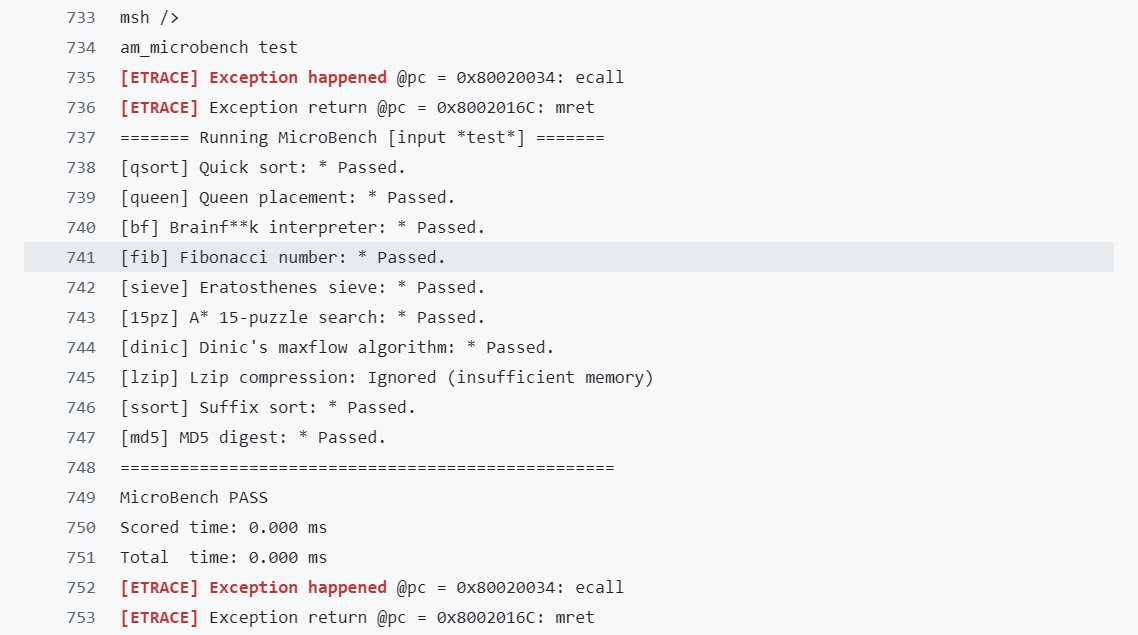
\includegraphics[width=\linewidth]{verify/image26.png}
  \vspace{0.25em}
  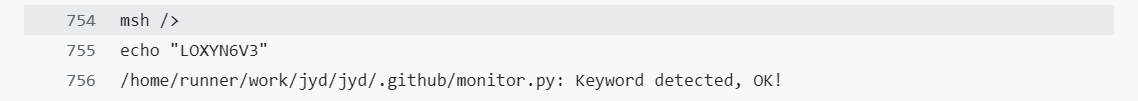
\includegraphics[width=\linewidth]{verify/image27.png}
  \caption{RT-Thread 自动化测试输出节选}
\end{figure}

自动化脚本向仿真串口依次输入命令并检查输出；version、free、hello、microbench 与 echo 均得到预期
结果。该测试同时覆盖 CSR、ecall/mret、上下文切换、堆管理、串口输入与较长程序执行。

\begin{figure}[H]
  \centering
  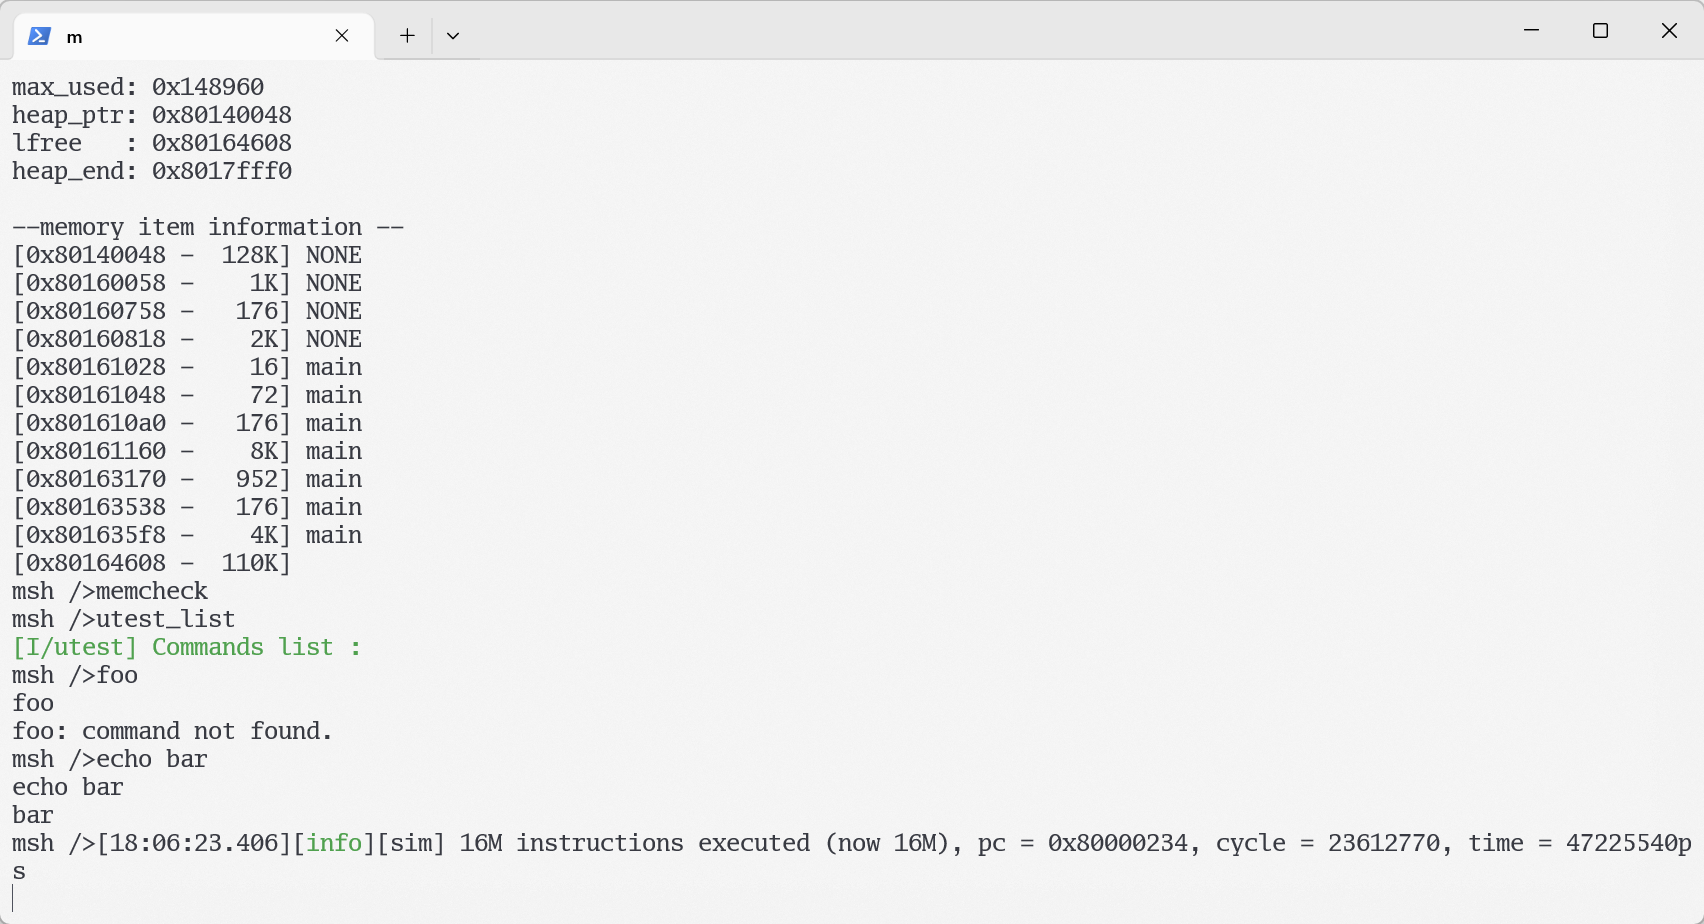
\includegraphics[width=0.9\linewidth]{verify/image28.png}
  \caption{RT-Thread 本地交互测试}
\end{figure}

\subsection{总决赛新增能力的验证闭环}

总决赛阶段在上述基础回归上新增 512 项 BTB/RAS 的预测与更新测试、4\,KiB 双 bank D-cache 的一致性
测试、RV32M 多周期 RAW 测试、已实现 B 扩展的指令语义测试，以及每条自定义指令的参考模型测试。
正式性能负载运行前先完成短迭代差分与 16M 指令前缀检查，再生成带身份记录的 bitstream；板测采用
10000 次迭代，要求 list、matrix、state 和 final 四项 CRC 全部正确，并用多次 capture 检查重复性。

\begin{table}[H]\centering
\caption{当前验证证据状态}\label{tab:verification-status}
\small
\begin{tabularx}{\linewidth}{@{}p{0.24\linewidth}p{0.14\linewidth}Y@{}}
\toprule
\textbf{证据项}&\textbf{状态}&\textbf{说明}\\\midrule
基础指令与 CPU tests&完成&覆盖算术、访存、分支、递归及相关边界\\
RV32M 与多周期 RAW&完成&包含 mul/mulh/mulhu/mulhsu 定向测试和握手停顿\\
CSR 与 RT-Thread&完成&可进入 shell 并执行代表性命令\\
自定义指令短迭代与前缀差分&完成&语义、CRC、访存副作用及 16M 指令前缀一致\\
正式负载多次板测&完成&最佳阶段三次相同 6.696371860\,s，四项 CRC 一致\\
250 MHz 完整实现&完成&post-route physical optimization WNS $+0.009$ ns\\
300 MHz 完整实现&完成&post-route physical optimization WNS $-0.580$ ns\\
当前资源利用率图&\MetricPending{提取}&补充 LUT、FF、BRAM、DSP 和时钟资源截图\\
\bottomrule
\end{tabularx}
\end{table}

\subsection{测评结果判读规则}

性能时间仅在程序输出和 CRC 校验通过后有效；仿真周期换算注明目标频率以及是否包含启动和输出开销；
板测优先使用硬件计时器与 UART 原始输出。WNS 注明时钟约束和报告阶段，routed 与 post-route physical
optimization 不混称。正文中的最终表格与图均可通过附录证据编号回查到相应实现报告或测评记录。

\clearpage
\section{总结}

本项目完成了一款面向 FPGA 的五级顺序单发射 RISC-V 处理器。处理器以 ready/valid 反压和 epoch
重定向维持顺序执行，通过 512 项 8-bank BTB、2-bit 动态方向预测和返回地址栈改善控制流，通过
两项固定槽取指缓冲隔离译码反压，通过总容量 4\,KiB 的双 bank D-cache、同步普通加载通路和链表查询
镜像副本服务两类不同访存需求，并以分区结果通路控制后端选择器深度和扇出。CSR 读改写局部化到
EXU，两阶段事务在执行级完成读取、准备和顺序提交。

指令能力覆盖 RV32I、RV32M、Zicsr、机器态控制流以及部分 RISC-V B 扩展。自定义指令包括 CRC 字节
更新、融合矩阵乘法/乘累加、链式查询与反转、矩阵归约和流式状态处理；各单元均纳入处理器的握手、相关检测、
访存一致性和顺序写回体系。GCC 工具链能够生成相应自定义指令，使硬件能力以统一的指令接口使用。

总决赛保留链的真实板测时间由 10.695831\,s 降至 5.346451\,s，缩短约 50.01\%。最终合入提交
\code{8591368} 完成流水边界、缓存查询、自定义加速和 GCC 中端/后端生成路径的整合；其 RTL 在
240\,MHz 下 routed WNS 为 $+0.014$\,ns 并完成时序收敛，在 300\,MHz 下 routed WNS 为
$-0.699$\,ns。最终程序的 10/100 次 NPC 仿射拟合为 5.292462350\,s，
NEMU 10,000 次回归 CRC 正确，但该时间尚未上板，文中始终以青色与真实板测分开。

验证体系覆盖 Vivado Simulation、Verilator/NEMU 差分测试、指令与体系结构测试、CoreMark、
Dhrystone、RT-Thread Nano 3.1.5、Vivado 实现和真实 FPGA 板测。由程序镜像、实现报告、bitstream 身份、UART
原始输出和 CRC 组成的证据链，使功能、性能与物理实现结果能够在统一口径下复核。对只改变编译器和
程序镜像、未改变 RTL 的最终迁移，复用已有实现 WNS 并明确标注未重跑 Vivado；没有板级 capture 的
拟合结果不表述为板测结论。

\clearpage
\appendix
\section{附录}

\subsection{分赛区后续性能与 WNS 演进}

本节完整保留《分赛区决赛后续优化说明报告》的两套量化结果。\texttt{withMext-v2} 用于贯穿分赛区
主报告版本至后续版本的统一 RTL 仿真复测；西北赛区样例用于观察不同访存与分支组成下的效果。
两套样例的绝对时间不可横向比较，折线只展示各自内部的性能与 WNS 变化。

\begin{table}[H]
  \centering
  \caption{统一采用 withMext-v2 的完整 RTL 仿真性能演进}
  \scriptsize
  \setlength{\tabcolsep}{4pt}
  \resizebox{\textwidth}{!}{%
  \begin{tabular}{@{}lcccc@{}}
      \toprule
      优化里程碑 & 频率 & 仿真时间 & 较前基线提升 & 时序状态 \\
      \midrule
      主报告版本 & 280 MHz & 2.020 s & --- & WNS $+0.050$ ns \\
      乘法与方向预测优化 & 280 MHz & 1.943 s & $3.8\%$ & WNS $+0.031$ ns \\
      D-cache 整字写分配 & 280 MHz & 1.868 s & $3.9\%$ & WNS $+0.019$ ns \\
      load-use 晚数据旁路 & 280 MHz & 1.643 s & $12.0\%$ & WNS $-0.084$ ns \\
      迭代 RTL 除法器 & 280 MHz & 1.606910 s & $2.2\%$ & 通过 \\
      LSU 地址通路与 280 MHz 收敛 & 280 MHz & 1.606910 s & $0.0\%$ & WNS $0.000$ ns \\
      窄加载与 D-cache shadow & 280 MHz & 1.607404 s & $-0.031\%$ & WNS $0.000$ ns \\
      32 项 BTB 与更新 shadow & 280 MHz & 1.607403 s & $+0.000055\%$ & WNS $-0.011$ ns \\
      精确 ret 识别与预测 & 280 MHz & 1.607403 s & $+0.000013\%$ & WNS $-0.091$ ns \\
      部分写命中保留 & 280 MHz & 1.607403 s & $+0.000001\%$ & WNS $-0.072$ ns \\
      接口缩减与除法修正分拍 & 280 MHz & 1.607403 s & $-0.000003\%$ & WNS $-0.004$ ns \\
      \textbf{最终时序闭合结果} & \textbf{280 MHz} & \textbf{1.607403 s} & $0.0\%$ & WNS $+0.013$ ns \\
      \bottomrule
  \end{tabular}}
\end{table}

最终结果完整运行 450,072,868 周期、380,344,384 条指令，CPI 为 1.183330；相对 2.020\,s
基线缩短约 20.4\%。后期若干节点主要用于时序与资源整理，因此保留精确百分比，避免将时序优化误写
成性能收益。

\begin{table}[H]
  \centering
  \caption{西北赛区样例的性能与时序演进}
  \small
  \setlength{\tabcolsep}{5pt}
  \begin{tabular}{@{}lccc@{}}
    \toprule
    优化里程碑 & 评估时间 & 较前基线提升 & 时序状态 \\
    \midrule
    多周期单元与 280 MHz 收敛 & 6.866 s & --- & WNS $0.000$ ns \\
    窄加载与 D-cache shadow & 6.553 s & $4.6\%$ & WNS $0.000$ ns \\
    32 项 BTB 与更新 shadow & 6.508 s & $0.7\%$ & WNS $-0.011$ ns \\
    精确 ret 识别与预测 & 6.481 s & $0.4\%$ & WNS $-0.091$ ns \\
    部分写命中保留 & 6.182 s & $4.6\%$ & WNS $-0.072$ ns \\
    \textbf{接口整理与最终时序闭合} & \textbf{6.184 s} & $-0.03\%$ & WNS $+0.013$ ns \\
    \bottomrule
  \end{tabular}
\end{table}

最终结果相对 6.866\,s 基线缩短约 9.9\%。6.182\,s 到 6.184\,s 的变化来自除法修正分拍和接口
整理；每次普通除法或求余增加一拍，完整前缀中 12 次相关操作精确增加 12 周期，同时 WNS 收敛至
$+0.013$\,ns。

\begin{figure}[H]
  \centering
  \begin{tikzpicture}
    \begin{axis}[
      width=0.835\textwidth,height=6.2cm,
      symbolic x coords={主报告,乘分支,DCache,晚旁路,LSU地址通路,Shadow,BTB,Ret,部分写,最终},
      xtick=data,x tick label style={rotate=32,anchor=east,font=\scriptsize},
      ylabel={评估时间（s）},ymin=1.55,ymax=2.05,
      axis y line*=left,axis x line*=bottom,grid=major,
      legend style={at={(0,1.02)},anchor=south west,font=\scriptsize}]
      \addplot[blue!75!black,mark=*] coordinates {
        (主报告,2.020) (乘分支,1.943) (DCache,1.868) (晚旁路,1.643)
        (LSU地址通路,1.606910) (Shadow,1.607404) (BTB,1.607403) (Ret,1.607403)
        (部分写,1.607403) (最终,1.607403)};
      \addlegendentry{性能}
    \end{axis}
    \begin{axis}[
      width=0.835\textwidth,height=6.2cm,
      symbolic x coords={主报告,乘分支,DCache,晚旁路,LSU地址通路,Shadow,BTB,Ret,部分写,最终},
      xtick=\empty,ylabel={WNS（ns）},ymin=-0.11,ymax=0.07,
      axis y line*=right,axis x line=none,
      legend style={at={(1,1.02)},anchor=south east,font=\scriptsize}]
      \draw[gray,dashed] (rel axis cs:0,0.6111) -- (rel axis cs:1,0.6111);
      \addplot[red!75!black,dashed,mark=square*] coordinates {
        (主报告,0.050) (乘分支,0.031) (DCache,0.019) (晚旁路,-0.084)
        (LSU地址通路,0.000) (Shadow,0.000) (BTB,-0.011) (Ret,-0.091)
        (部分写,-0.072) (最终,0.013)};
      \addlegendentry{WNS}
    \end{axis}
  \end{tikzpicture}
  \caption{withMext-v2 的性能与 WNS 走向}
\end{figure}

\begin{figure}[H]
  \centering
  \begin{tikzpicture}
    \begin{axis}[
      width=0.835\textwidth,height=6.0cm,
      symbolic x coords={时序基线,窄加载,BTB,Ret,部分写,最终},
      xtick=data,x tick label style={rotate=25,anchor=east,font=\scriptsize},
      ylabel={评估时间（s）},ymin=6.05,ymax=6.95,
      axis y line*=left,axis x line*=bottom,grid=major,
      legend style={at={(0,1.02)},anchor=south west,font=\scriptsize}]
      \addplot[blue!75!black,mark=*] coordinates {
        (时序基线,6.866) (窄加载,6.553) (BTB,6.508) (Ret,6.481) (部分写,6.182) (最终,6.184)};
      \addlegendentry{性能}
    \end{axis}
    \begin{axis}[
      width=0.835\textwidth,height=6.0cm,
      symbolic x coords={时序基线,窄加载,BTB,Ret,部分写,最终},
      xtick=\empty,ylabel={WNS（ns）},ymin=-0.11,ymax=0.04,
      axis y line*=right,axis x line=none,
      legend style={at={(1,1.02)},anchor=south east,font=\scriptsize}]
      \draw[gray,dashed] (rel axis cs:0,0.7333) -- (rel axis cs:1,0.7333);
      \addplot[red!75!black,dashed,mark=square*] coordinates {
        (时序基线,0.000) (窄加载,0.000) (BTB,-0.011) (Ret,-0.091)
        (部分写,-0.072) (最终,0.013)};
      \addlegendentry{WNS}
    \end{axis}
  \end{tikzpicture}
  \caption{西北赛区样例的性能与 WNS 走向}
\end{figure}


\subsection{硬件加速构建配置摘要}\label{app:accel-build}

项目借助 GCC 目标选项和相关接口，按处理器提供的硬件能力配置程序镜像。启用与关闭版本采用相同输入、
迭代规模和结果判定；该配置不改变处理器 RTL。

最终构建以固定工具链、选项和程序镜像完成回归。NPC 的 10/100 次运行均通过差分与 CRC 校验，
NEMU 10,000 次运行通过相同 CRC；同时检查程序镜像摘要和构建日志，确保复测使用的二进制与
记录一致。正文据此报告硬件功能、流水边界、性能结果和验证范围。
\subsection{自动化验证截图（补充证据）}

下列两图保留分赛区阶段的可视化记录，用于展示测试输出形式。它们不替代正文中按提交标识、
任务链接、日志摘录和计数器构成的最新可复现证据。

\begin{figure}[H]
  \centering
  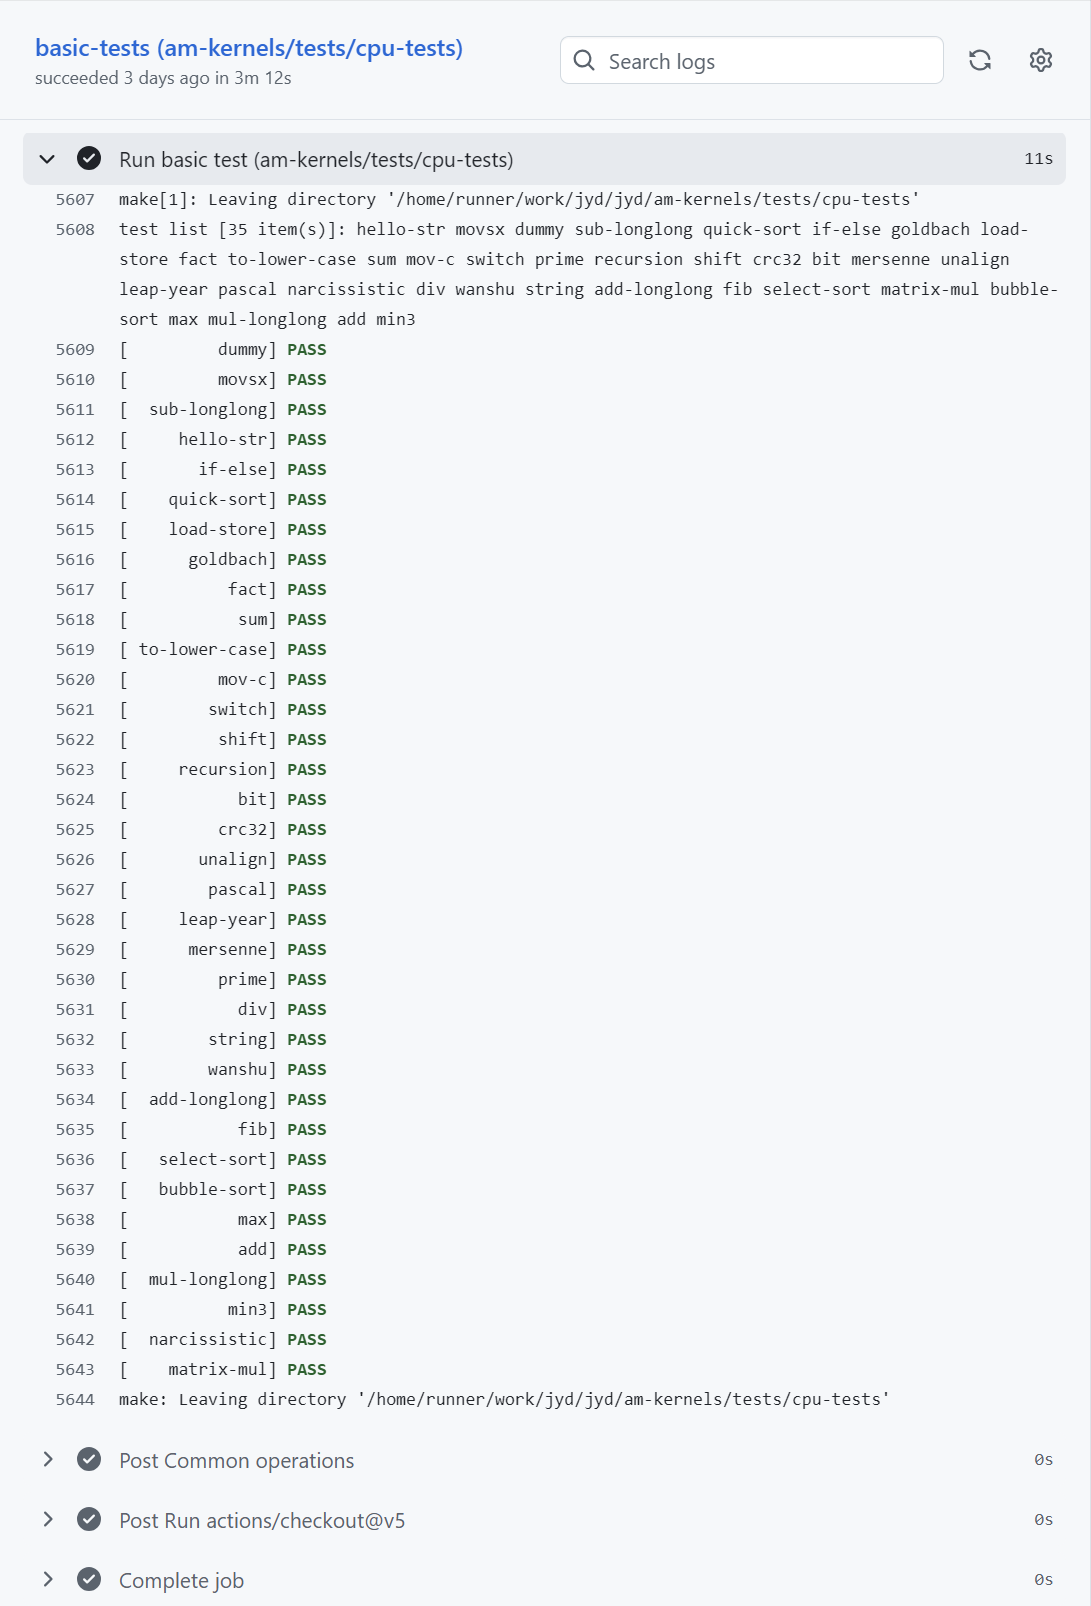
\includegraphics[height=0.58\textheight,trim=0 0 669bp 0,clip]{verify/image13.png}%
  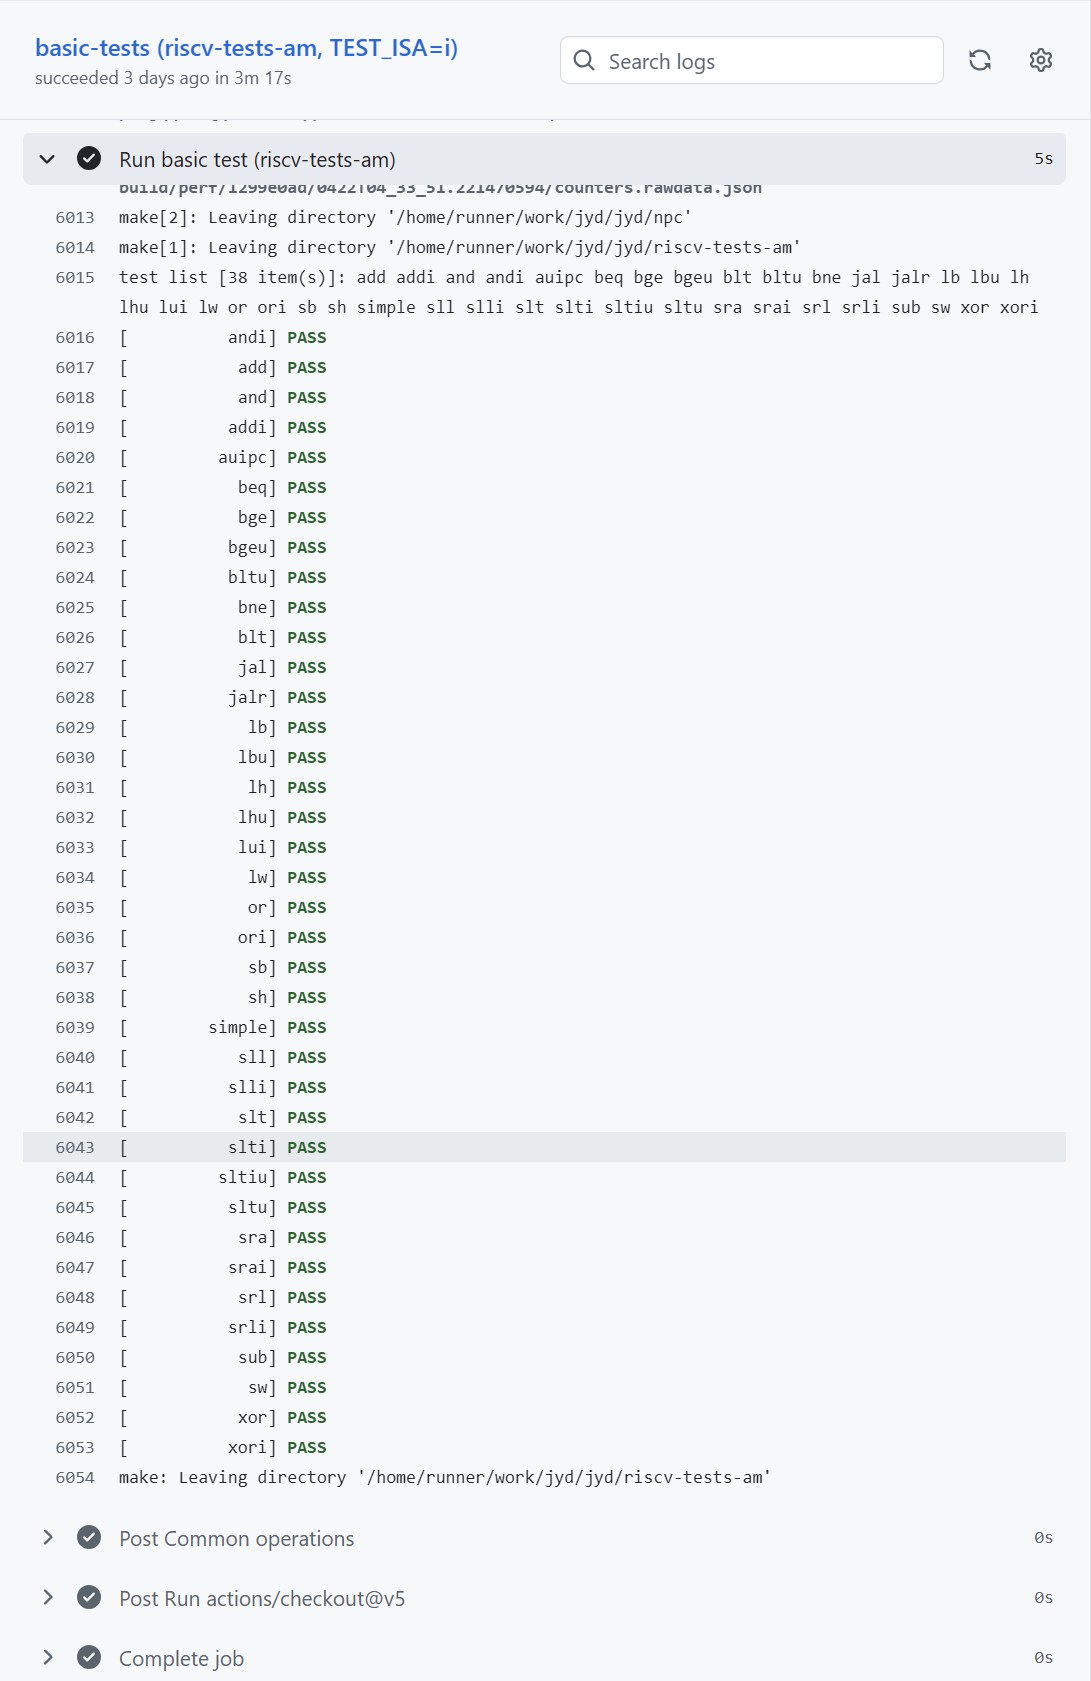
\includegraphics[height=0.58\textheight,trim=0 0 644bp 0,clip]{verify/image14.png}%
  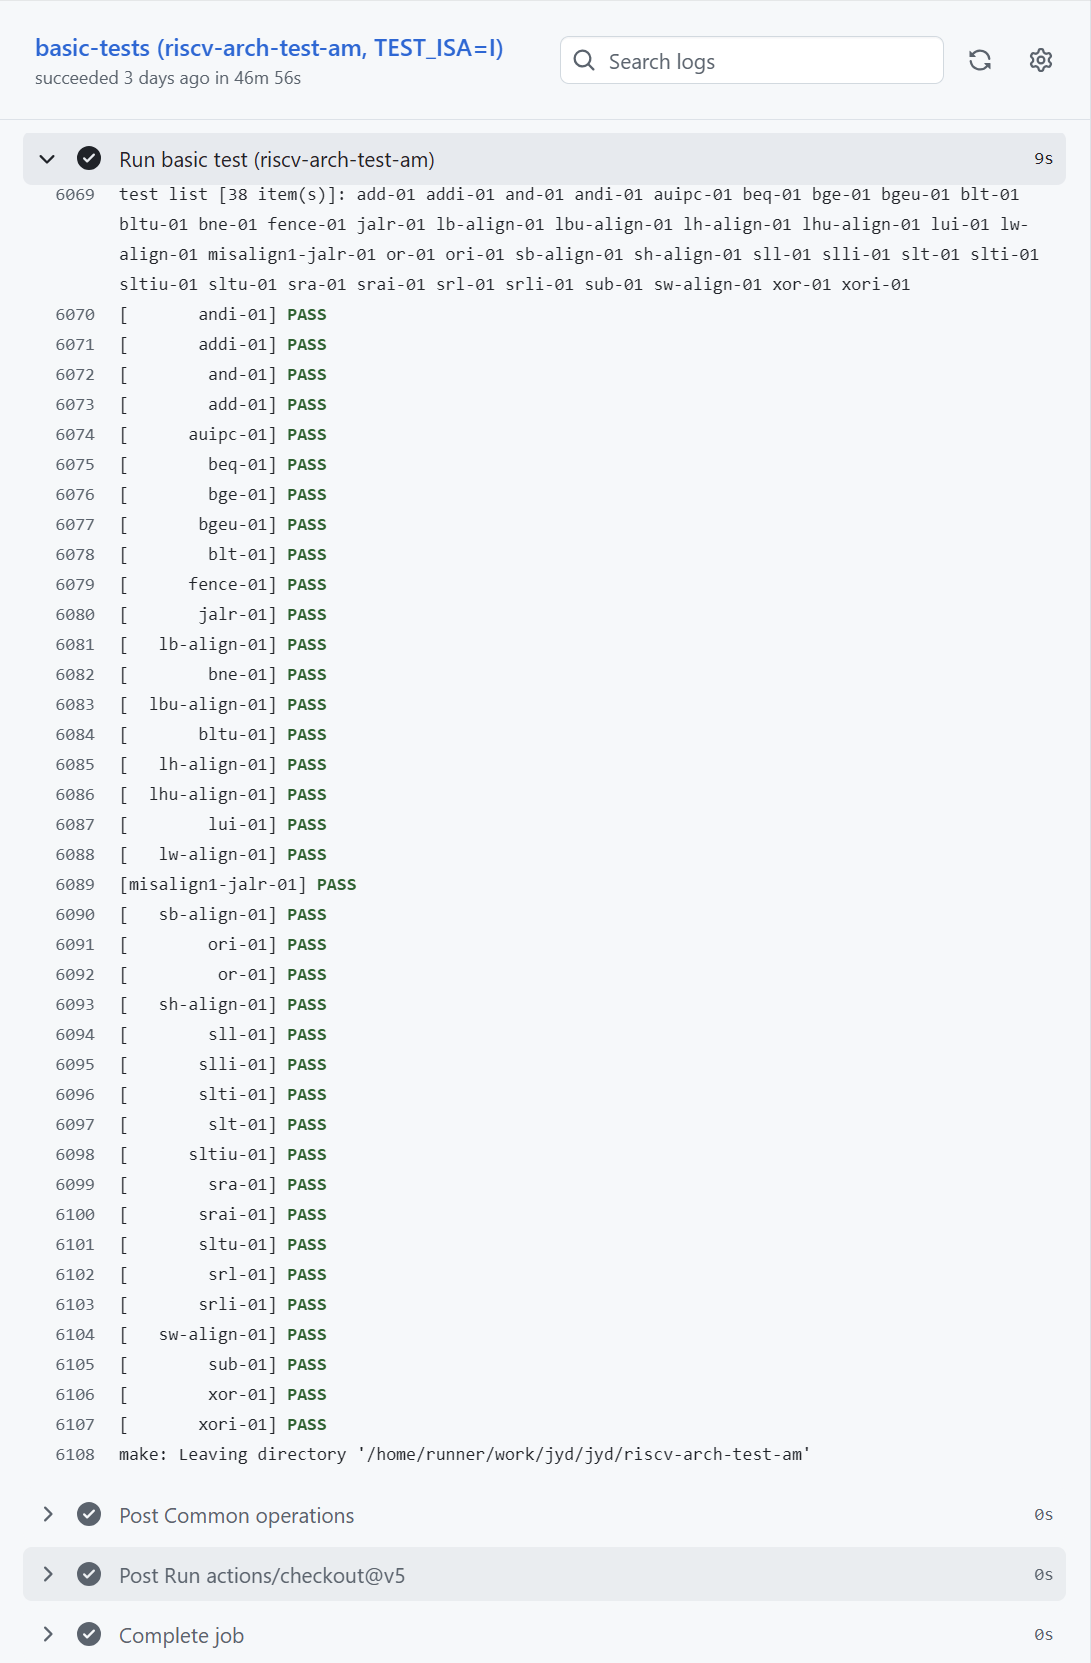
\includegraphics[height=0.58\textheight,trim=0 0 654bp 0,clip]{verify/image15.png}
  \caption{RV32I 基本指令测试结果}
\end{figure}

\begin{figure}[H]
  \centering
  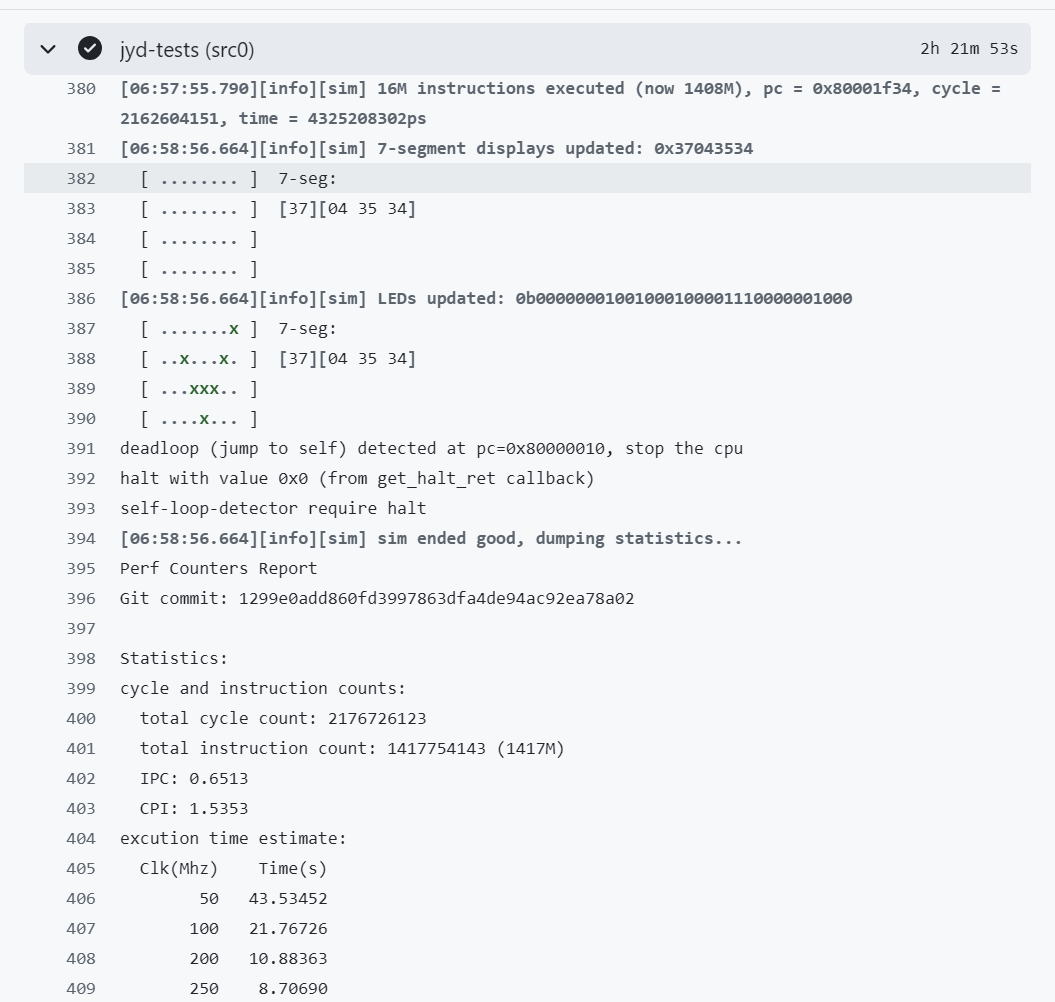
\includegraphics[width=0.82\linewidth,trim=0 365bp 0 0,clip]{verify/image16.png}
  \caption{src0 仿真日志与性能统计}
\end{figure}

\subsection{测评证据索引}

\begin{table}[H]\centering
\caption{关键测评证据索引}
\scriptsize
\setlength{\tabcolsep}{3pt}
\resizebox{\linewidth}{!}{\begin{tabular}{@{}lll@{}}
\toprule
\textbf{编号}&\textbf{证据类型}&\textbf{用途}\\\midrule
E-FINAL-240&最终合入 RTL 的 240 MHz 实现归档&routed WNS $+0.014$ ns、TNS 0、无失败端点\\
E-FINAL-300&300 MHz 实现归档&routed/post-physopt WNS $-0.590/-0.580$ ns\\
E-FINAL-CUR&最终合入 RTL 实现归档&routed WNS $-0.699$ ns；最终构建配置未改变 RTL\\
E-RF-01--04&分赛区后续报告与统计数据&withMext-v2、西北样例的性能与 WNS 演进\\
E-BOARD-01&最佳阶段 UART 板测归档&6.696371860\,s、四项 CRC、板卡与 bitstream 身份\\
E-BOARD-02&正确 IP 板级复测归档&6.714950940\,s、四项 CRC、300\,MHz 实现与 bitstream 身份\\
E-BOARD-03&加速接口构建的同硬件对照&6.691154040\,s、三次一致、四项 CRC 与程序镜像身份\\
E-BOARD-COMB&组合加速板测归档&5.346451040\,s、三次一致、四项 CRC 与修正后的 COE 身份\\
E-CI-01&GitHub Actions 可复现回归&run 31680203475、提交 75329078；无硬件加速 CoreMark 5,000 次迭代及其他负载日志与计数器\\
E-CI-ACC&较早硬件加速自动化回归&run 31708291526、任务 94474591976、提交 fa30e65e；5,000 次迭代日志与完整计数器\\
E-CAND-01&当前文档对应版本&最终合入提交 8591368；包含 RTL 结构与加速接口配置\\
E-ACCEL-FINAL&最终加速构建回归&NPC 10/100 次、5.292462350\,s 拟合值、NEMU 10,000 次及镜像身份检查\\
E-PROF-CRC&CRC 热点画像与板测记录&5,840,008 次动态操作、内联溢出访存和同 ISA 板测对照\\
E-PROF-COMPUTE&定宽计算与顺序访存画像&29.16M 次位域乘法及 12.96M 个处理元素\\
E-PROF-STREAM&流式状态定向周期记录&10,000-call 软件/硬件周期及处理字节计数\\
E-PROF-DEPEND&早期依赖访存原型评估&61.2M 个读写步骤及串行访存净周期代价\\
E-PROF-BACKEND&后端分区实现审计&routed WNS/TNS、失败端点数及 16M 指令周期对照\\
E-TEST&自动化测试记录&基础指令、CPU tests 与体系结构测试输出\\
E-RTTNANO&系统移植与运行记录&Nano 3.1.5 固定版本；NEMU 命令通过、最终 RTL 启动及 D-cache 断言边界\\
\bottomrule
\end{tabular}}
\end{table}

文档外的工程归档保存精确版本标识、程序镜像摘要、bitstream 摘要和原始日志，便于团队内部复核；
正文仅保留评审理解设计与测评口径所需的信息。机器可读证据清单位于 \code{src/data/evidence.csv}。

\subsection{工程目录结构}

\makeatletter
\newcommand{\mydotfill}{%
  \leavevmode
  \leaders\hbox to 1em{\hss\raisebox{0.3ex}{\textcolor{gray}{.}}\hss}\hfill\kern0pt}
\makeatother

\noindent\begin{minipage}{0.96\textwidth}
\small
\dirtree{%
.1 jyd/ \mydotfill 工程根目录.
.2 npc/ \mydotfill CPU、SoC 封装与仿真工程.
.3 design/src/ \mydotfill 流水线、预测器、缓存、扩展与设备描述.
.3 build/gened/verilog/ \mydotfill 生成的 Verilog/SystemVerilog.
.3 sim/ \mydotfill Verilator 仿真、差分与性能统计.
.3 scripts/ \mydotfill 打包、实现、报告提取与板测脚本.
.2 nemu/ \mydotfill RISC-V 参考执行环境.
.2 sdb/ \mydotfill 差分状态、调试器与指令环.
.2 abstract-machine/ \mydotfill 裸机运行环境与 riscv32-jyd 平台.
.2 jyd-tests/rtthread-nano/ \mydotfill RT-Thread Nano 3.1.5 的 AM 移植与系统测试.
.2 jyd-vivado-proj/ \mydotfill 数字孪生 Vivado 工程、IP 与约束.
.2 doc/Finals/final-rpt/ \mydotfill 总决赛技术文档.
.3 src/chapters/ \mydotfill 分章节正文.
.3 src/tikz/ \mydotfill 独立管理的 TikZ/pgfplots 图源.
.3 src/assets/ \mydotfill 仿真截图、波形、照片与外部图片.
.3 src/data/ \mydotfill 性能、时序和证据索引数据.
}
\end{minipage}

\clearpage
\subsection{参考资料}

\small
\begin{enumerate}[label={\textup{[\arabic*]}},leftmargin=3em,itemsep=0.08em,topsep=0.2em]
  \item 全国大学生集成电路创新创业大赛组委会：《第十届集创赛作品提交要求》。
  \item 竞业达企业命题组：《竞业达企业命题作品材料参考模板》。
  \item 竞业达企业命题组：《FPGA 开发板远程连接操作手册》，2026。
  \item RISC-V International, \emph{The RISC-V Instruction Set Manual, Volume I: Unprivileged ISA}.
  \item RISC-V International, \emph{The RISC-V Instruction Set Manual, Volume II: Privileged Architecture}.
  \item AMD Xilinx, \emph{Vivado Design Suite User Guide: Design Analysis and Closure Techniques}.
  \item AMD Xilinx, \emph{7 Series FPGAs Memory Resources User Guide}.
  \item EEMBC, \emph{CoreMark: An EEMBC Benchmark},
  \href{https://github.com/eembc/coremark}{official source and run rules}.
  \item Reinhold P. Weicker, ``DHRYSTONE: A Synthetic Systems Programming Benchmark,''
  \emph{Communications of the ACM}, 27(10), 1984,
  DOI: \href{https://doi.org/10.1145/358274.358283}{10.1145/358274.358283}.
  \item Verilator Project, \emph{Verilator User's Guide},
  \href{https://verilator.org/guide/latest/}{latest online edition}.
  \item Nanjing University ProjectN, \emph{NEMU: Nanjing University Emulator},
  \href{https://github.com/NJU-ProjectN/nemu}{official repository}.
  \item RT-Thread Project, \emph{RT-Thread Nano v3.1.5},
  \href{https://github.com/RT-Thread/rtthread-nano/tree/v3.1.5}{official source archive}.
  \item RISC-V International, \emph{RISC-V Architecture Test},
  \href{https://github.com/riscv-non-isa/riscv-arch-test}{official repository}; RISC-V Software,
  \href{https://github.com/riscv-software-src/riscv-tests}{riscv-tests}.
  \item Nanjing University ProjectN, \emph{AbstractMachine},
  \href{https://github.com/NJU-ProjectN/abstract-machine}{official repository}.
  \item Nanjing University ProjectN, \emph{PA: RT-Thread 选做讲义},
  \href{https://ysyx.oscc.cc/docs/ics-pa/4.1.html\#rt-thread-\%E9\%80\%89\%E5\%81\%9A}{online course notes}.
  \item Nanjing University ProjectN, \emph{rt-thread-am},
  \href{https://github.com/NJU-ProjectN/rt-thread-am}{teaching branch adapted to AbstractMachine}.
  \item Nanjing University ProjectN, \emph{riscv-tests-am},
  \href{https://github.com/NJU-ProjectN/riscv-tests-am}{riscv-tests port for AbstractMachine}.
  \item Nanjing University ProjectN, \emph{riscv-arch-test-am},
  \href{https://github.com/NJU-ProjectN/riscv-arch-test-am}{architecture-test port for AbstractMachine}.
  \item Nanjing University ProjectN, \emph{am-kernels},
  \href{https://github.com/NJU-ProjectN/am-kernels}{AbstractMachine kernels and cpu-tests}.
  \item Chisel Project, \emph{Chisel Documentation},
  \href{https://www.chisel-lang.org/docs}{official documentation}.
  \item GitHub, \emph{Using workflow run logs},
  \href{https://docs.github.com/en/actions/how-tos/monitor-workflows/use-workflow-run-logs}{GitHub Actions documentation};
  \href{https://github.com/HanPiM/jyd/actions/runs/31680203475}{run 31680203475}.
\end{enumerate}
\normalsize

\clearpage
\subsection{AI 工具使用声明}

项目研发和技术文档整理过程中使用 OpenAI 的 ChatGPT/Codex 系列工具提供辅助。分赛区阶段主要使用
ChatGPT（GPT-4o），总决赛阶段主要使用 Codex（GPT-5 系列，Codex CLI 0.147.0）；版本号按实际使用
阶段记录，云端模型的小版本由服务端滚动更新。团队对体系结构决策、代码合入、测试结果和最终文字负责，
AI 工具不替代人工设计评审、功能验证、FPGA 实现或板级测评。

按各类工作的投入量粗略估算，AI 辅助约占：体系结构分析与优化决策 15\%，RTL/工具链/脚本代码编写与
修改 30\%，验证方案与日志整理 30\%，技术文档文字、LaTeX 排版和 TikZ 图表 60\%；折合项目总体工作量
约 25\%。这些比例表示工具参与草拟、检索或整理的工作量，不表示内容未经人工复核。主要用途如下：

\begin{itemize}
  \item \textbf{工程检索与影响分析：}辅助定位模块连接、接口定义、测试入口和实现报告中的关键路径；
  \item \textbf{脚本与重复性工作：}辅助编写 COE 转换、日志整理、报告字段提取、批量回归和文档审计脚本；
  \item \textbf{代码初稿与局部重构：}依据团队给出的结构方案生成局部实现草稿，再由团队审阅、修改和测试；
  \item \textbf{验证用例补充：}辅助整理边界条件、RAW 相关、握手反压、缓存一致性和硬件加速单元参考语义；
  \item \textbf{时序报告解读：}辅助汇总逻辑级数、布线占比、端点族和资源变化，优化方向由团队确定；
  \item \textbf{技术文档编排：}辅助章节结构、表格排版、术语一致性检查、TikZ/pgfplots 图表草拟与文字润色；
  \item \textbf{使用边界：}性能与 WNS 数据均来自仿真、Vivado 报告或板测原始记录；指令语义、接口时序和
  硬件结构均经过团队审核，不使用 AI 生成的虚构数据或未经验证的结论。
\end{itemize}

\end{document}
